
\documentclass[a4paper,twoside,11pt]{report}      % Comments after  % are ignored
%\usepackage{hyperref}                 % For creating hyperlinks in cross references
% 

\usepackage{lipsum}
\usepackage{tocloft}

\makeatletter
\def\@makechapterhead#1{%
  \vspace*{50\p@}%
  {\parindent \z@ \raggedright \normalfont
    \interlinepenalty\@M
    \Large \bfseries #1\par\nobreak
    \vskip 40\p@
  }}
\def\@makeschapterhead#1{%
  \vspace*{50\p@}%
  {\parindent \z@ \raggedright
    \normalfont
    \interlinepenalty\@M
    \Large \bfseries  #1\par\nobreak
    \vskip 40\p@
  }}
\makeatother



\usepackage{ifxetex}% for XELATEX, or PDFlatex
\usepackage{ifplatform} 
\usepackage{pst-optic} 
\usepackage{pstricks}
\usepackage[bottom]{footmisc}
\usepackage[newparttoc]{titlesec}
%
\ifxetex
	\usepackage{polyglossia} \setmainlanguage{portuges}
	\usepackage{fontspec}
	\ifwindows
		\setmainfont[Ligatures=TeX]{Garamond}
		\setsansfont[Ligatures=TeX]{Gill Sans MT}
%	\setmonofont[Scale=MatchLowercase]{Courier}
		\setmonofont[Scale=0.95]{Courier}
	\fi
	\iflinux
		\setmainfont[Ligatures=TeX]{Linux Libertine O}
		\setsansfont[Ligatures=TeX,Scale=MatchLowercase]{Linux Biolinum}
		\setmonofont[Scale=MatchLowercase]{Courier}
	\fi
	\ifmacosx
	% add settings
	% Use xelatex -no-shell ...
	\fi
	\usepackage{xcolor,graphicx} 
\else
	\usepackage[portuguese]{babel}
	%\usepackage[latin1]{inputenc}
	\usepackage[utf8]{inputenc}
	\usepackage[T1]{fontenc}
	\usepackage{graphics}                 % Packages to allow inclusion of graphics
	\usepackage{color}                    % For creating coloured text and background
\fi

%\makeatletter
%\@addtoreset{chapter}{part}
%\makeatother 

\usepackage{enumitem}
\setlist{nolistsep}

\usepackage[retainorgcmds]{IEEEtrantools}
\usepackage{tikz}
\usetikzlibrary{calc,arrows,decorations.pathmorphing,intersections}
\usepackage[font={small,sf},labelfont={bf},labelsep=endash]{caption}
\usepackage{sansmath}


\usepackage{amsmath,amssymb,amsfonts} % Typical maths resource packages
\usepackage{multicol}

\oddsidemargin 0cm
\evensidemargin 0cm

\pagestyle{myheadings}         % Option to put page headers
                               % Needed \documentclass[a4paper,twoside]{article}
\markboth{{LEFT}}
{{\small\it \protect\input{../../LIFE.txt}}}

\textwidth 15.5cm
\topmargin -1cm
\parindent 0.5cm
\textheight 24cm
\parskip 1mm

\usepackage{enumitem}
\setlist{nolistsep}

%\usepackage{textcomp}

% Math macros
\newcommand{\ud}{\,\mathrm{d}} 
\newcommand{\HRule}{\rule{\linewidth}{0.5mm}}

\author{Prof. Bernardo B. Carvalho} 

\begin{document} 
\thispagestyle{empty} 
	\includegraphics[width=0.2\textwidth]{../../logo-ist}%\\[1cm]  %%  Logo_IST_color
%%%%%%%%%%%%%%%%%%%%%%%%%%%%%%%%%%%%%%%%%%%%%%%%%
%%%%%%%%%%%%%%%%%%%%%%%%%%%%%%%%%%%%%%%%%%%%%%%%%
%%%%%%%%%%%%%%%%%%%%%%%%%%%%%%%%%%%%%%%%%%%%%%%%%
%%%%%%%%%%%%%%%%%%%%%%%%%%%%%%%%%%%%%%%%%%%%%%%%%
%%%%%%%%%%%%%%%%%%%%%%%%%%%%%%%%%%%%%%%%%%%%%%%%%
%%%%%%%%%%%%%%%%%%%%%%%%%%%%%%%%%%%%%%%%%%%%%%%%%
%%%%%%%%%%%%%%%%%%%%%%%%%%%%%%%%%%%%%%%%%%%%%%%%%
%%%%%%%%%%%%%%%%%%%%%%%%%%%%%%%%%%%%%%%%%%%%%%%%%
%%%%%%%%%%%%%%%%%%%%%%%%%%%%%%%%%%%%%%%%%%%%%%%%%
%%%%%%%%%%%%%%%%%%%%%%%%%%%%%%%%%%%%%%%%%%%%%%%%%

\begin{center}
\vspace{2cm}
 {\Huge \bf{Laboratório de Introdução à}}\\
  {\Huge \bf{Física Experimental}}\\
\vspace{1cm}
 {\large \bf{Licenciatura em Eng. Física Tecnológica}}\\
\vspace{2cm}
 \begin{figure}[htb] 
	\centering 
	
\includegraphics[width=1.0\textwidth]{cover} 
\end{figure}


 {\huge \bf{Guias das experiências}}\\
 \vspace{2cm}
 {\large \bf{2.º semestre 2022/2023}}\\
\end{center}

\newpage
 \vspace{4cm}
\tableofcontents

\HRule \\[0.5cm]
\chapter{ \huge{Experiência de Thomson}}
\large {\bf {Determinação experimental da relação $q/m$ do electrão}}\\
\HRule \\%[0.5cm]

\section{\sf Objectivo do trabalho}
Pretende-se com este trabalho determinar a relação entre a carga e a massa ($q/m$) do electrão. Para esse fim, vamos estudar a deflexão de um feixe de raios catódicos sob o efeito de um campo eléctrico e de um campo magnético.

\section{\sf Conceitos fundamentais}
Os raios catódicos foram descobertos em 1879 por William Crookes (1832--1919), mas foi Sir J. J. Thomson\footnote{Prémio Nobel da Física de 1906, em reconhecimento dos seus trabalhos teóricos e experimentais na condução da electricidade em gases.} (1856--1940) que, em 1897, relatou as experiências por si realizadas e que permitiram determinar o valor daquela relação. Além disso, estas experiências provaram que os raios catódicos são constituídos por partículas de carga negativa, desde então designadas por electrões. Neste trabalho iremos reproduzir aproximadamente a experiência de Thomson.

%\section{\sf Introdução}
%\subsection*{\sf  Conceitos necessários:} 
%\begin{enumerate}
%	\item Força eléctrica. Campo electrostático.
%	\item Potencial eléctrico. Equipotencial. Energia potencial eléctrica.
%	\item Condutores e dieléctricos. Condensador plano.
%	\item Efeitos da corrente eléctrica estacionária criada por uma espira. 	
%	\item Força de Lorentz.
%\end{enumerate}

\subsection{\sf Campo electrostático}

Define-se como sendo o campo eléctrico criado por uma distribuição de cargas que \emph{não evolui no tempo}. Considere-se por exemplo o par de cargas $q_1$ e $q_2$ imersas no vácuo, à distância $r_{12}$, e situadas respetivamente em $P_1$ e $P_2$, conforme ilustrado na Fig. \ref{fig:fig1}. A força eléctrica que sofre $q_1$ no ponto $P_1$ devido a $q_2$ em $P_2$ à distância $r_{12}$ é
\begin{equation}
	\vec{F}_{P_1,q_1} (q_2, r_{1 2} ) =\frac{1}{4 \pi \varepsilon_0}\frac{q_1 q_2}{r_{1 2}^2} \vec{u}_{r,P_1} = 
	- \vec{F}_{P_2,q_2} (q_1, r_{1 2} )
%	B = \mu H \to H= \sqrt{\frac{ \varepsilon}{\mu}} E 
\end{equation}
em que $\varepsilon_0$  é designada por constante dieléctrica ou permitividade eléctrica do vazio ($\varepsilon_0 \simeq 8,854 \cdot 10^{-12}$ F/m) e $\vec{u}_{r,P_1}$  é o \emph{versor} da distância $r_{1 2} $ no ponto $P_1$  (vector unitário dirigido de $P_2$ para $P_1$, ver figura).

%\begin{minipage}[b]{0.5\linewidth}
Dada uma carga $q_1$ e um ponto $P$ a uma distância $r$, define-se o \emph{campo eléctrico} $\vec{E}$  em $P$ como a força eléctrica por unidade de carga exercida sobre uma carga de prova ou teste, suposta unitária e positiva, colocada em $P$:
\begin{equation}
	\vec{E}_P (q_1, r) = \frac{q_1}{4 \pi \varepsilon_0 r^2} \vec{u}_{r, P} 
\end{equation}
As unidades do campo eléctrico são o newton/coulomb (N/C) ou, mais habitualmente, o volt/metro (V/m).

As linhas de força eléctrica geradas por $q_1$ são radiais e dirigidas para o exterior, se $q_1>0$, ou para a origem, se $q_1<0$. Se se colocasse em $P$  a carga $q$,  a força eléctrica a que esta carga ficaria submetida devido a $q_1$  seria	
$\vec{F}_{P,q} (q_1, r ) = q \vec{E}$, 
ou mais simplesmente:
\begin{equation}
\vec{F} = q \vec{E}
\end{equation}
A expressão ``campo eléctrico" também define a região do espaço onde se fazem sentir as acções eléctricas.
\begin{figure}[t]
  \centering 
	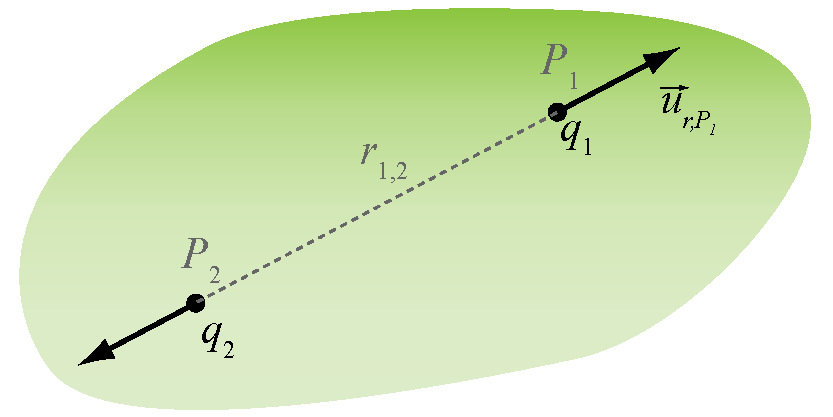
\includegraphics[width=0.5\textwidth]{./fig1-thomson} 
	\caption{ Definição dos termos para a geometria de duas cargas. \label{fig:fig1}} 

\end{figure}


\subsection{\sf Potencial eléctrico}
	
O campo eléctrico e a força eléctrica, que são entidades vectoriais, podem também ser calculadas a partir de uma função capaz de descrever o campo mas de natureza escalar, o \emph{potencial eléctrico} $V$. Para a situação referida acima, o potencial eléctrico criado no ponto $P$ à distância $r$ da carga $q_1$ é calculado por:
\begin{equation} \label{eq:pot_ele}
	V_P (q_1, r) = \frac{q_1}{4 \pi \varepsilon_0 r} 
\end{equation}


No caso de uma distribuição de $n$ cargas eléctricas $q_i$ à distância $r_i$ do ponto $P$ onde se pretende calcular o campo eléctrico e o potencial, tem-se:
\begin{align}
	\vec{E}_P &= \frac{1}{4 \pi \varepsilon_0 } \sum_{i=1}^n \Big( \frac{q_i}{ r_i^2}\; \vec{u}_{r_i , P}  \Big) \nonumber \\ 
 V_P &= \frac{1}{4 \pi \varepsilon_0 } \sum_{i=1}^n \Big( \frac{q_i}{ r_i}  \Big) \nonumber
\end{align}

Recorde-se que se se considera uma única carga $q_1$ positiva, as linhas de força eléctricas são radiais e dirigidas para o exterior. Essas linhas de força são perpendiculares às \emph{superfícies equipotenciais}, que são esféricas ($r = \mathrm{c.^{te}}$ na equação \ref{eq:pot_ele}) e concêntricas com as cargas. Atendendo a (\ref{eq:pot_ele}) para dois raios $r_1$ e $r_2$ tal que $r_2 > r_1$ temos $V(r_2) < V(r_1)$, e portanto as linhas de força dirigem-se para os potenciais decrescentes.

Considere-se agora o caso de duas cargas $q_1 > 0$ e $q_2 < 0$. Enquanto estiverem muito afastadas uma da outra, produzem campos radiais, respetivamente divergindo e convergindo. Se forem colocadas suficientemente próximas, as linhas de força vão sofrer a influência de ambas as cargas. Nesse caso, apenas uma única linha de força é linear, dirigida de $q_1$ para $q_2$. Todas as outras, que na vizinhança próxima de cada carga são radiais, acabam por infletir, dirigindo-se de $q_1$ para $q_2$. A figura das linhas de força tem simetria de revolução em torno do eixo que contém $q_1$ e $q_2$ e é esquematicamente a indicada na Fig. \ref{fig:sup-equip}. Se o valor absoluto das duas cargas for o mesmo a figura é simétrica em relação ao plano mediatriz das cargas $q_1$ e $q_2$ \footnote{Para mais exemplos ver https://phet.colorado.edu/en/simulations/charges-and-fields}.

\begin{figure}[tb]
  \centering 
	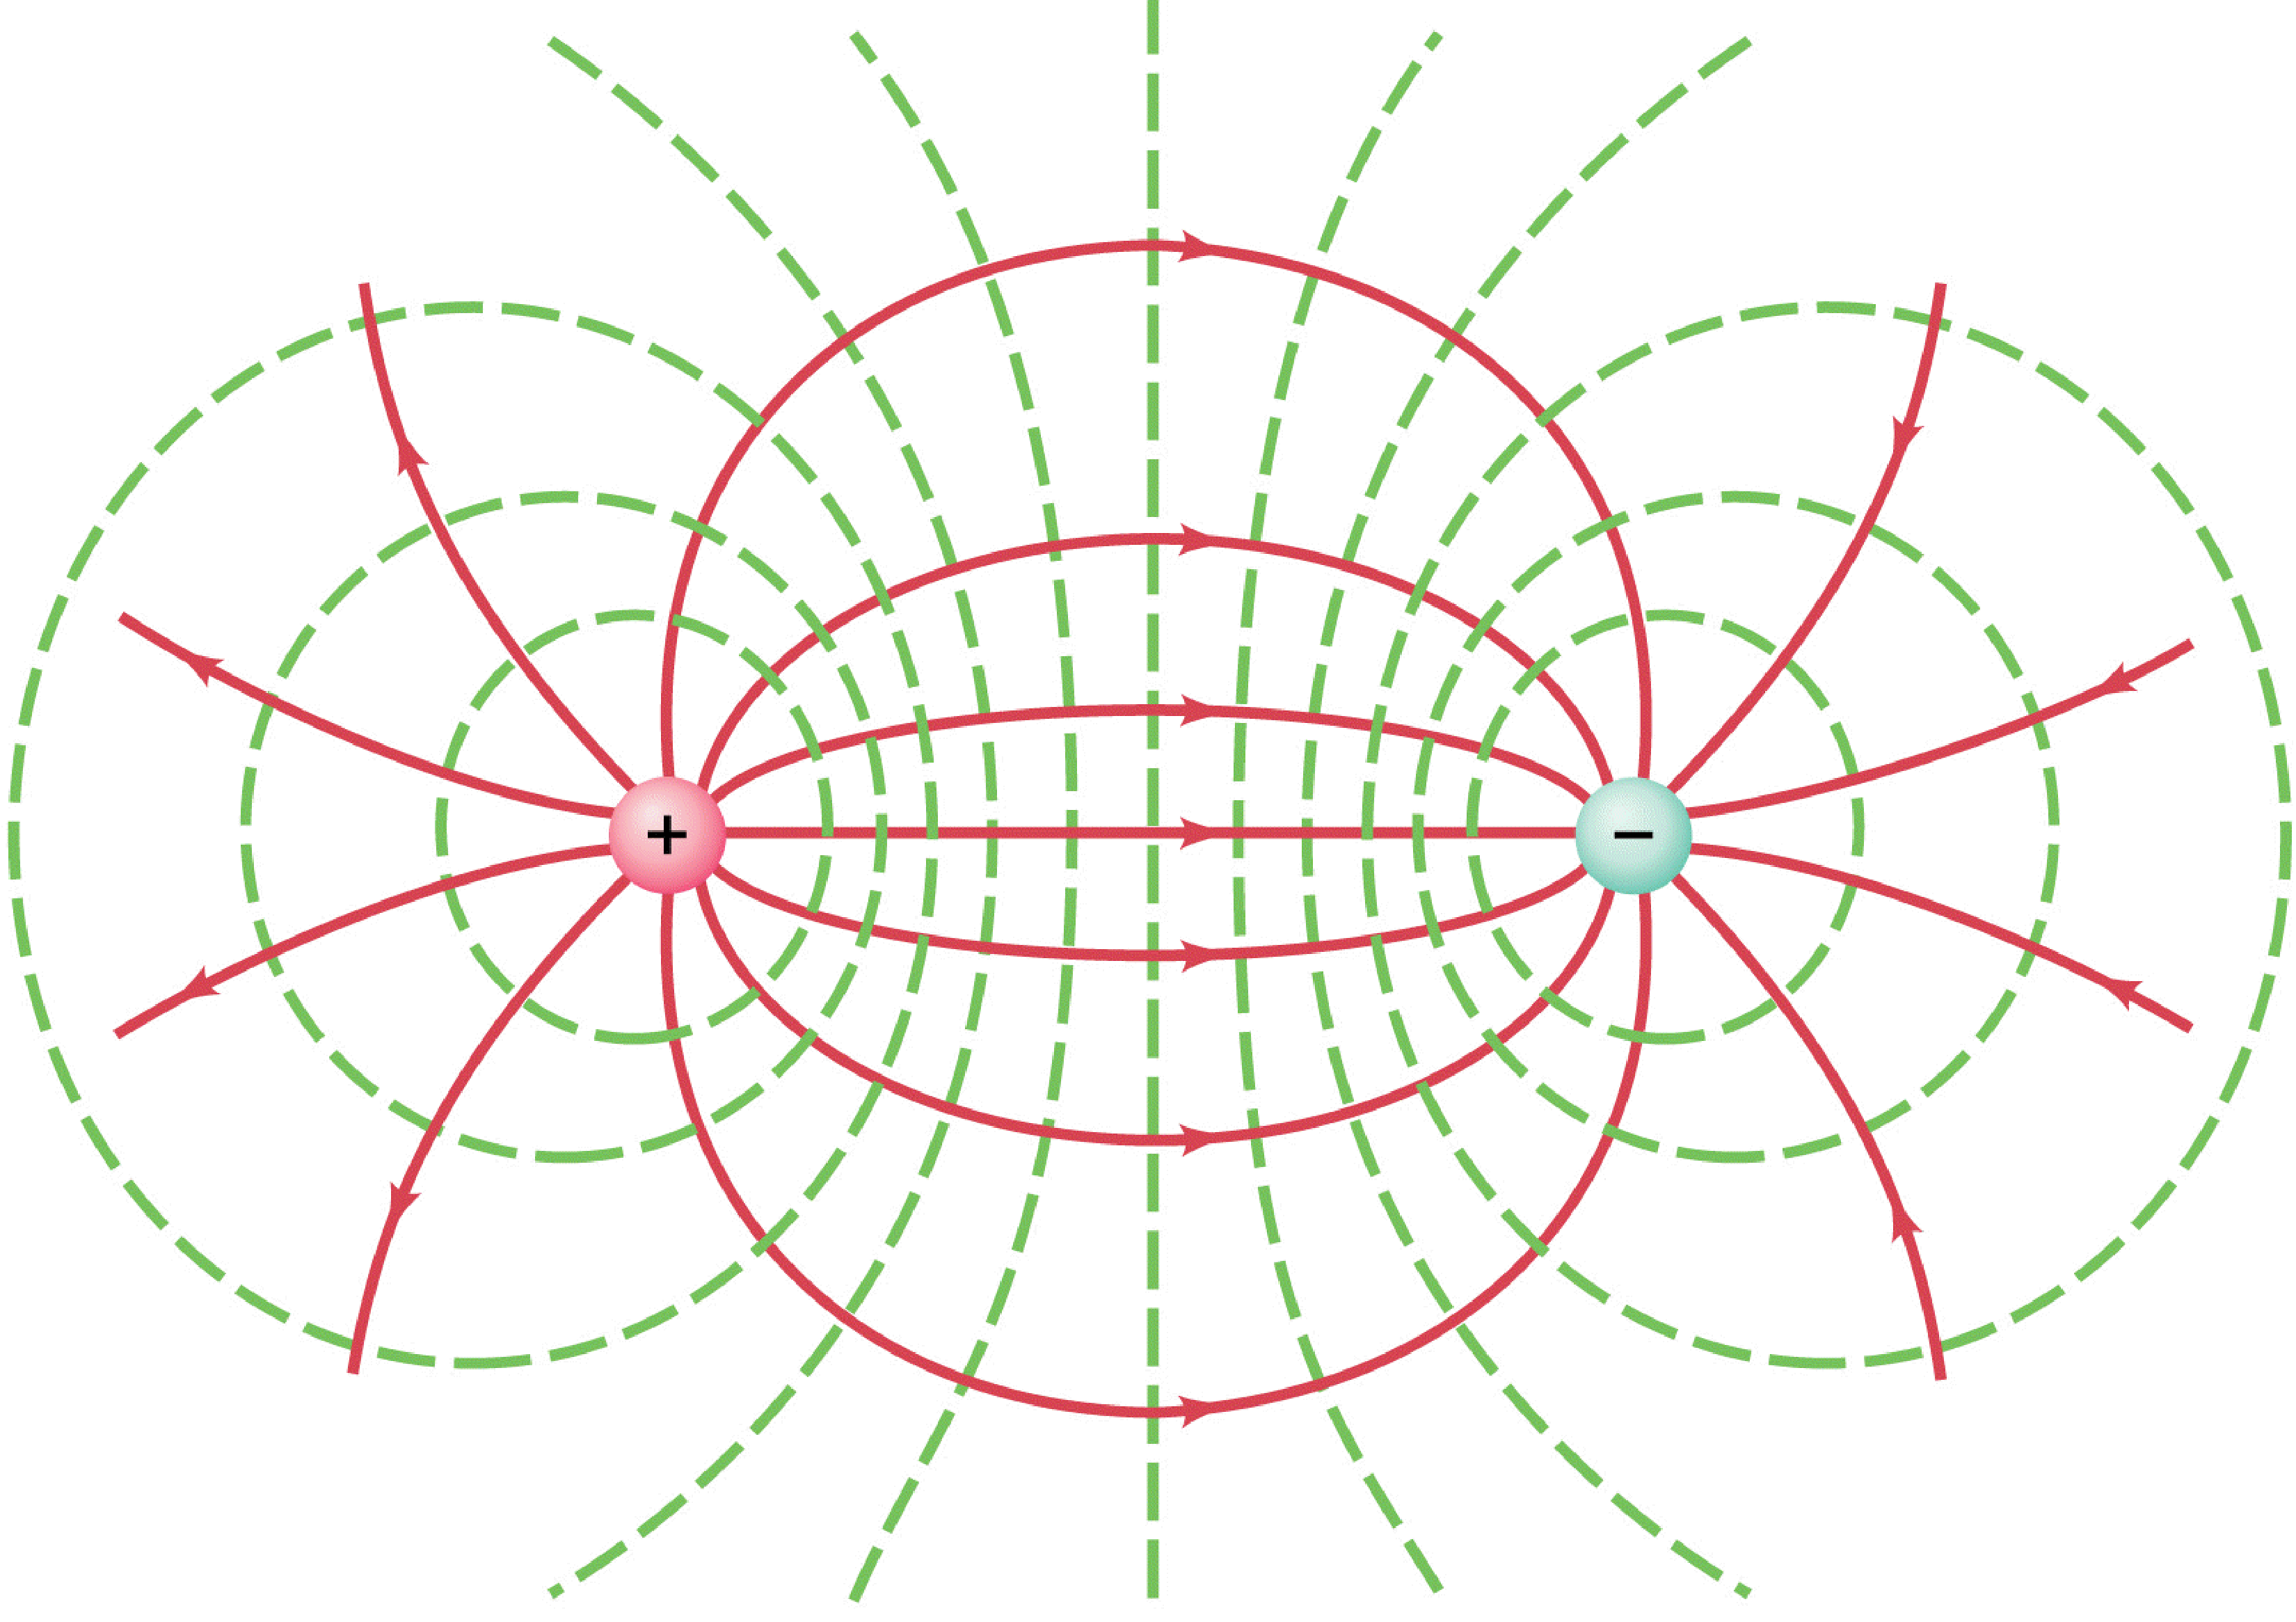
\includegraphics[width=0.5\textwidth]{./fig2-thomson} 
	\caption{ Linhas de força (a vermelho) e superfícies equipotenciais (a verde) de duas cargas simétricas. \label{fig:sup-equip}} 
\end{figure}

Se se calcular a diferença de potencial entre dois pontos infinitamente próximos $P$ e $P+dP$ devida a uma carga $q_1$ à distância $r$ e $r+dr$ respetivamente, a variação elementar do potencial $V$ será:
%\begin{minipage}[b]{0.45\linewidth}
\begin{align}
d V &= V_{P+dP} - V_P = \frac{q_1}{4 \pi \varepsilon_0 r} \big(  \frac{1}{r + dr} -\frac{1}{r} \big)\nonumber\\
	 &\approx \frac{q_1}{4 \pi \varepsilon_0 } \big(  - \frac{dr}{r^2} \big) = - \vec{E} \cdot d \vec{r}  \end{align}

Esta quantidade representa o trabalho elementar (energia) associado ao deslocamento da
carga teste ($q_t=1\,$ C), de $P$ para $P+dP$. Para $q_1 > 0$,	$\vec{E}$ e $\vec{dr}$ são paralelos e $dV < 0$. Isto significa que
não será necessário fornecer energia para realizar esse transporte. 
De facto, afastar a carga teste da carga $q_1$ (i.e. ir de $P$ para $P+dP$) leva a uma configuração de cargas ($q_1$ e $q_t$) energeticamente mais favorável \footnote{Recorde-se que para um campo conservativo o trabalho realizado (que não depende do percurso mas só dos pontos inicial e final) tem um valor simétrico da variação de energia potencial.}.

No caso de uma diferença finita de potencial, isto é de uma diferença de potencial entre dois pontos $P$ e $Q$, ter-se-á que somar um número infinito de contribuições infinitesimais $dV_i=- \vec{E}_i \cdot d\vec{r}_i$ no intervalo de $P$ a $Q$:

\begin{equation}
V_Q-V_P  = \lim_{n  \to \infty } \sum_{i=1}^n dV_i = \lim_{n \to \infty } \sum_{i=1}^n \underbrace{( - \vec{E}_i \cdot d\vec{r}_i )}_{\overline{PQ}} \rightarrow \int - \vec{E} \cdot d\vec{r}
\end{equation}
%\frown 

\begin{equation*} 
V_P - V_Q  = \int_{\overline{PQ}}  \vec{E} \cdot d \vec{r}
\end{equation*}
e porque $\vec{E}$ (campo electrostático) é um campo conservativo, este integral não vai depender do percurso mas apenas dos pontos extremos, i.e.
\begin{equation*} 
V_P - V_Q  = \int_P^Q  \vec{E} \cdot d\vec{r}
\end{equation*}


No caso particular de $E$ ser homogéneo (por exemplo no interior de um condensador plano)  na região onde se situam os pontos $P$ e $Q$, afastados de uma distância $D$, obtém-se 
\begin{equation}\label{eq:difPot}
V_P - V_Q  =  \vec{E}\cdot\vec{PQ}=E\cdot D
\end{equation}

Para se compreender o significado físico de $V_P$, imagine-se que $Q$ é um ponto infinitamente
afastado da região em que se faz sentir o campo eléctrico $\vec{E}$.
Nesse ponto, $r \to \infty $ e $V_Q=0$,
obtendo-se $V_P =  \int_P^\infty  \vec{E} \cdot d\vec{r}$, que permite a seguinte interpretação:
\newline
\newline
\fbox {\begin{minipage}{36em}
O potencial eléctrico $V_P$ é a energia necessária para transportar a carga-teste, sob acção de $\vec{E}$, desde o ponto $P$ até uma distância suficientemente grande tal que o campo eléctrico não se faça sentir.
\end{minipage}}
\newline
\newline
Assim, $V$ tem sempre o significado de uma diferença de potencial.

%Se for a carga $q_2$, a energia necessária será $W= q_2\cdot V$. 
\subsubsection{{\sf Energia electrostática}}
A energia associada a uma configuração de cargas $q_1$ e $q_2$, à distância $r$, é dada por:

\begin{equation}\label{eq:enrPot}
 W = \frac{q_1 q_2}{4 \pi \varepsilon_0 r} = q_1 V_1 = q_2 V_2 =  \frac{q_1 V_1 +q_2 V_2}{2} 
\end{equation}
em que $V_1$ é o potencial no ponto $P_1$ criado pela carga $q_2$, e $V_2$ é o potencial no ponto $P_2$ criado pela carga $q_1$. 

Recordando a definição do potencial criado por $n$ cargas eléctricas, podemos generalizar a equação (\ref{eq:enrPot}) na seguinte forma:

\begin{equation}%\label{eq:enrPot}
 W_E =  \frac{1}{2} \sum_{i,j (i\ne j)}^n \frac{ 1 }{4 \pi \varepsilon_0} \frac{ q_i \, q_j }{r_{i\,j}}  = 
	 \frac{1}{2} \sum_{i=1}^n q_i \left( \sum_{j \ne i}^n \frac{ q_j }{4 \pi \varepsilon_0 \,r_{i\,j}} \right) =
	\frac{1}{2} \sum_{i=1}^n q_i V_i
\end{equation}
que corresponde à energia necessária para criar a distribuição de cargas $q_i$. A energia $W_E$ é uma energia potencial porque está associada às posições que as diferentes cargas ocupam, podendo ser recuperada se as cargas se afastarem umas das outras até distâncias $r \to \infty$.

\subsection{\sf Condutores eléctricos e dieléctricos. Condensador plano}
Um material é um \emph{condutor eléctrico ideal} se as cargas eléctricas do mesmo sinal em excesso (que o carregam) são livres de se movimentarem no seu interior e à sua superfície. Quando pelo contrário isso não acontece, estamos perante um \emph{dieléctrico}.

Assim, se carregarmos um condutor com uma carga total $Q$ (se $Q > 0$, significa que se retiram electrões ao condutor inicialmente neutro) essas cargas, todas do mesmo sinal, vão
acomodar-se logo que se atinja o equilíbrio electrostático, em posições que são o mais afastadas possíveis umas das outras -- ou seja, na superfície exterior do condutor, formando uma ``folha'' de carga. Pode mostrar-se que $\vec{E}$ no interior do condutor é nulo (enquanto que num
dieléctrico $\vec{E} \ne \vec{0}$), e que a superfície do condutor é uma \emph{equipotencial}: logo, as linhas de força eléctricas são-lhe perpendiculares. Quando um material é carregado, a velocidade com que essas cargas se transferem de todo o volume do condutor para a superfície depende da sua condutividade. Se se considerar um condutor carregado, com geometria plana (uma placa), a carga vai distribuir-se sobre a superfície (ver ilustração em baixo).
\setlength{\unitlength}{0.8cm} 
\begin{center}
	\framebox[0.6\linewidth][c]{
		\begin{picture}(6,3)
		%\linethickness{0.075mm} 
		\put(1,1){\line(1,0){4}}
		\put(5,1){\line(0,1){1}}
		\put(5,2){\line(-1,0){4}}
		\put(1,2){\line(0,-1){1}}
		\multiput(1.1, 2.1)(.5, 0){8}{$+$}
		\multiput(1.1, 0.7)(.5, 0){8}{$+$}
		\put(.6,1.4){$+$}
		\put(5.0,1.4){$+$}
		\end{picture}
} 
\end{center}
Ao colocar-se em frente uma placa idêntica, mas de carga simétrica, haverá uma redistribuição de carga que produz um campo eléctrico tal como ilustrado em baixo. Na região central, as linhas de força são paralelas entre si e o campo eléctrico é homogéneo. Nas extremidades as linhas de força emergem perpendicularmente à superfície mas encurvam, deixando de ser lineares. Esta geometria e distribuição de carga são características de um \emph{condensador plano}. A diferença de potencial entre as duas placas, afastadas de $D$, corresponde a ($V_+ \,–\, V_-) = E\cdot D$, pois $\vec{E}$ é homogéneo (eq. \ref{eq:difPot}).\\
\setlength{\unitlength}{1.0cm} 
\begin{center}
	\framebox[0.6\linewidth][c]{
		\begin{picture}(6,5.5)
		%\linethickness{0.075mm} 
		\put(1,4){\line(1,0){4}}
		\put(5,4){\line(0,1){1}}
		\put(5,5){\line(-1,0){4}}
		\put(1,5){\line(0,-1){1}}
		\multiput(1.1, 3.7)(.5, 0){8}{$+$}
		\put(.65,4.4){$+$} \put(5.0,4.4){$+$}
		%
		\put(1,1){\line(1,0){4}}
		\put(5,1){\line(0,1){1}}
		\put(5,2){\line(-1,0){4}}
		\put(1,2){\line(0,-1){1}}
		\multiput(1.1, 2.1)(.5, 0){8}{$-$}
		\put(.7,1.4){$-$} \put(5.0,1.4){$-$}
		\color{red}
		\multiput(1.5, 3.7)(1, 0){4}{\vector(0,-1){1.5}}
		\qbezier(0.9,3.7)(0.7,2.95)(0.9,2.2)
		\put(.89,2.3){\vector(1,-2){0.1}}
		\qbezier(5.1,3.7)(5.3,2.95)(5.1,2.2)
		\put(5.11,2.3){\vector(-1,-2){0.1}}
		\put(4.7,2.5){$\vec{E}$}
		\end{picture}
	} 
\end{center}
Pode mostrar-se que $\vec{E}$ fica confinado à região entre as placas. Se o condensador fosse infinito (sem extremidades) teríamos três regiões, as duas exteriores ao condensador, onde o campo  $\vec{E}$  é nulo, e entre as placas do condensador (também designadas por armaduras), onde o campo seria homogéneo.


\subsection{\sf Efeitos da corrente eléctrica estacionária criada por uma espira}
A passagem da \emph{corrente eléctrica estacionária} (i.e. cuja intensidade não varia no tempo) por um condutor cria um campo magnético $\vec{B}$, além de produzir calor por efeito de Joule. As \emph{linhas de força magnética} produzidas por um fio condutor linear são circulares e concêntricas com o condutor (Fig. \ref{fig:condutor}). O módulo de $B$ num ponto a uma distância $r$ do fio (medida na perpendicular ao fio) é
\begin{equation}
	|\vec{B_{\mathrm{fio}}}| = \frac{\mu_0 I}{2\, \pi \, r} 
\end{equation}
 em que $\mu_0 =  4 \pi× 10^{−7}$ H/m é a \emph{permeabilidade magnética}  do vazio. 
 
 \begin{figure}[t]
	\centering 
	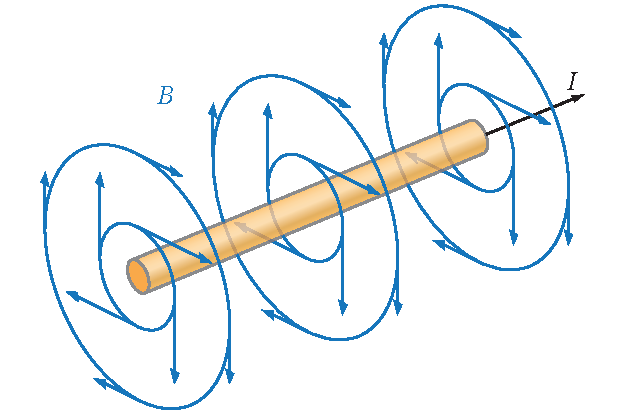
\includegraphics[width=0.5\textwidth]{fig-fio} 
	\caption{Campo magnético produzido por um fio onde passa corrente.}
	\label{fig:condutor}
\end{figure}

No caso de uma espira\footnote{Termo que designa um circuito eléctrico fechado} circular, é criado um campo magnético cujas linhas de força são curvas fora do seu eixo e lineares apenas ao longo do eixo (Fig. \ref{fig:espira1}). Pode provar-se que o campo magnético criado por uma espira de raio $r$, percorrida por uma corrente de intensidade $I$, tem linhas de força fechadas\footnote{Mesmo aquelas que só \emph{fecham} no infinito}, ao contrário das linhas de força eléctricas. Isto coloca em evidência que $\vec{B}$ nos pontos do plano da espira, mas exteriores a esta, é antiparalelo a $\vec{B}$ no eixo da espira (ver figura). O módulo de $\vec{B}$ num ponto do eixo é dado por
\begin{equation}
	|\vec{B}_{\mathrm{espira}}| = \frac{\mu_0 I}{2 r} \sin^3 \alpha
\end{equation}

 \begin{figure}[h]
  \centering 
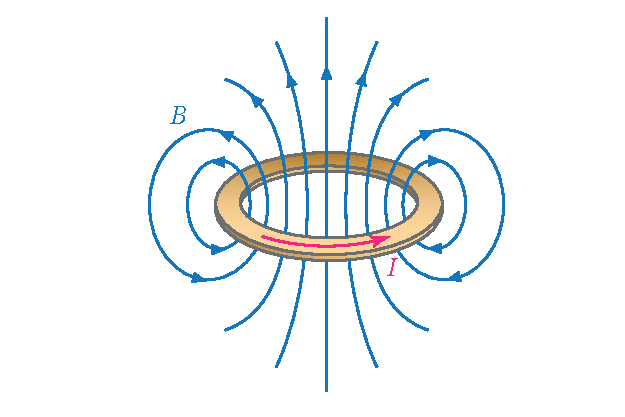
\includegraphics[width=0.5\textwidth]{fig-espira.pdf}
\caption{Campo magnético produzido por uma espira circular onde passa corrente.}
\label{fig:espira1}
\end{figure}

\subsection{\sf Força de Lorentz }
Uma carga q animada de uma velocidade $\vec{v}$ numa região em que existe um campo de indução $\vec{B}$ e um campo eléctrico $\vec{E}$ fica submetida a uma força de Lorentz\footnote{Se a força for apenas de origem magnética, $\vec{F}_m =  q\,(\vec{v} \times \vec{B})$, pode chamar-se também de \emph{Laplace}} $\vec{F}$ dada por:
\begin{equation}
	\label{eq:Lorentz}
 \vec{F} = q\; \vec{E} + q\,(\vec{v} \times \vec{B})
\end{equation}

A força de Lorentz resulta da soma vectorial de uma componente eléctrica e uma componente magnética, que verificam as seguintes propriedades:
\begin{itemize}
\item a força eléctrica $\vec{F_e}=q\vec{E}$ tem a mesma direção que o campo eléctrico; se a carga for positiva tem o mesmo sentido, se a carga for negativa tem o sentido oposto;
\item a força magnética $\vec{F_e}=q(\vec{v} \times \vec{B})$ é perpendicular ao plano definido pelos vectores velocidade $(\vec{v})$ e campo magnético $(\vec{B})$, sendo o seu sentido dado pela regra da mão direita para o produto externo de vectores.
\end{itemize}
Quando a velocidade da carga e o campo magnético são mutuamente perpendiculares, a força magnética comporta-se como uma força centrípeta e a carga descreve uma trajectória circular (ver Fig. \ref{fig:lorentz1}) cujo raio se pode calcular igualando os módulos das duas forças $(|\vec{F_c}|=|\vec{F_m})|$:

\begin{figure}[t]
  \centering 
	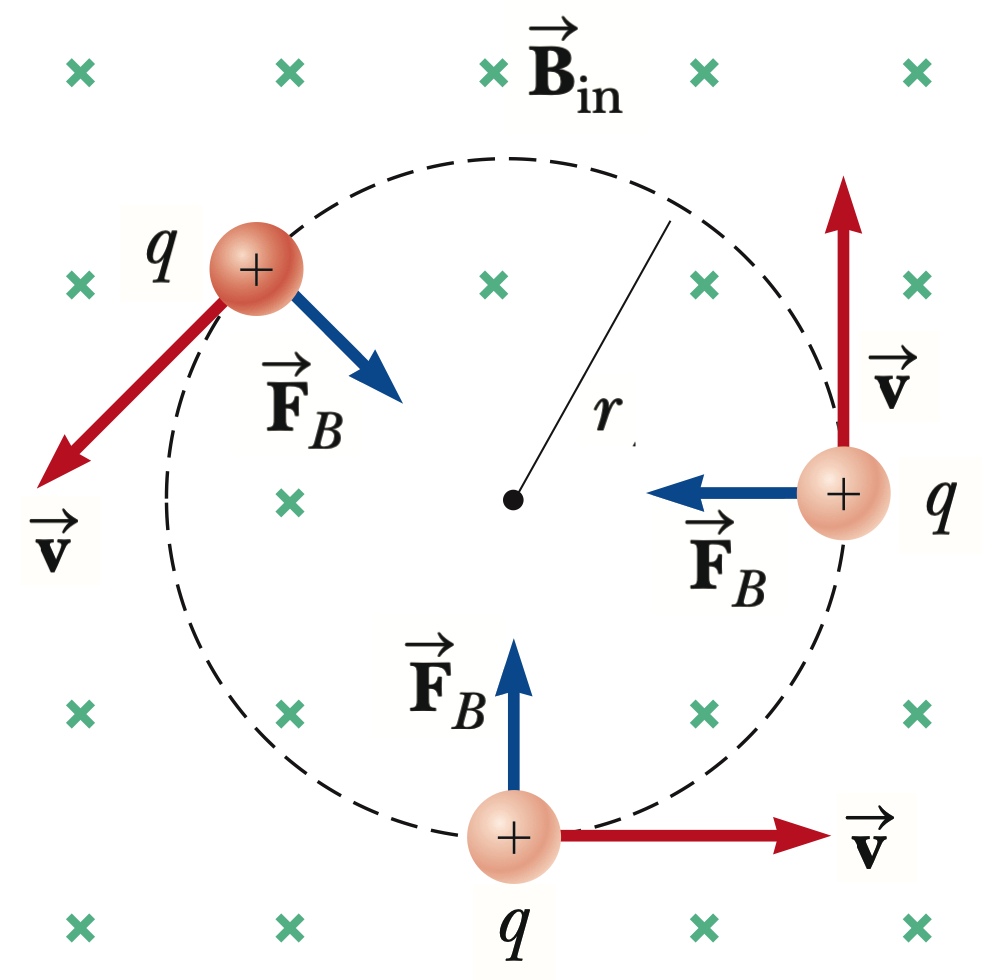
\includegraphics[width=0.4\textwidth]{./Lorentz1.png} 
	\caption{Trajectória circular para uma carga positiva $q$ com velocidade $\vec{v}$ na presença de um campo magnético $\vec{B}_{in}$ perpendicular. \label{fig:lorentz1}} 
\end{figure}

\begin{figure}[b]
  \centering 
	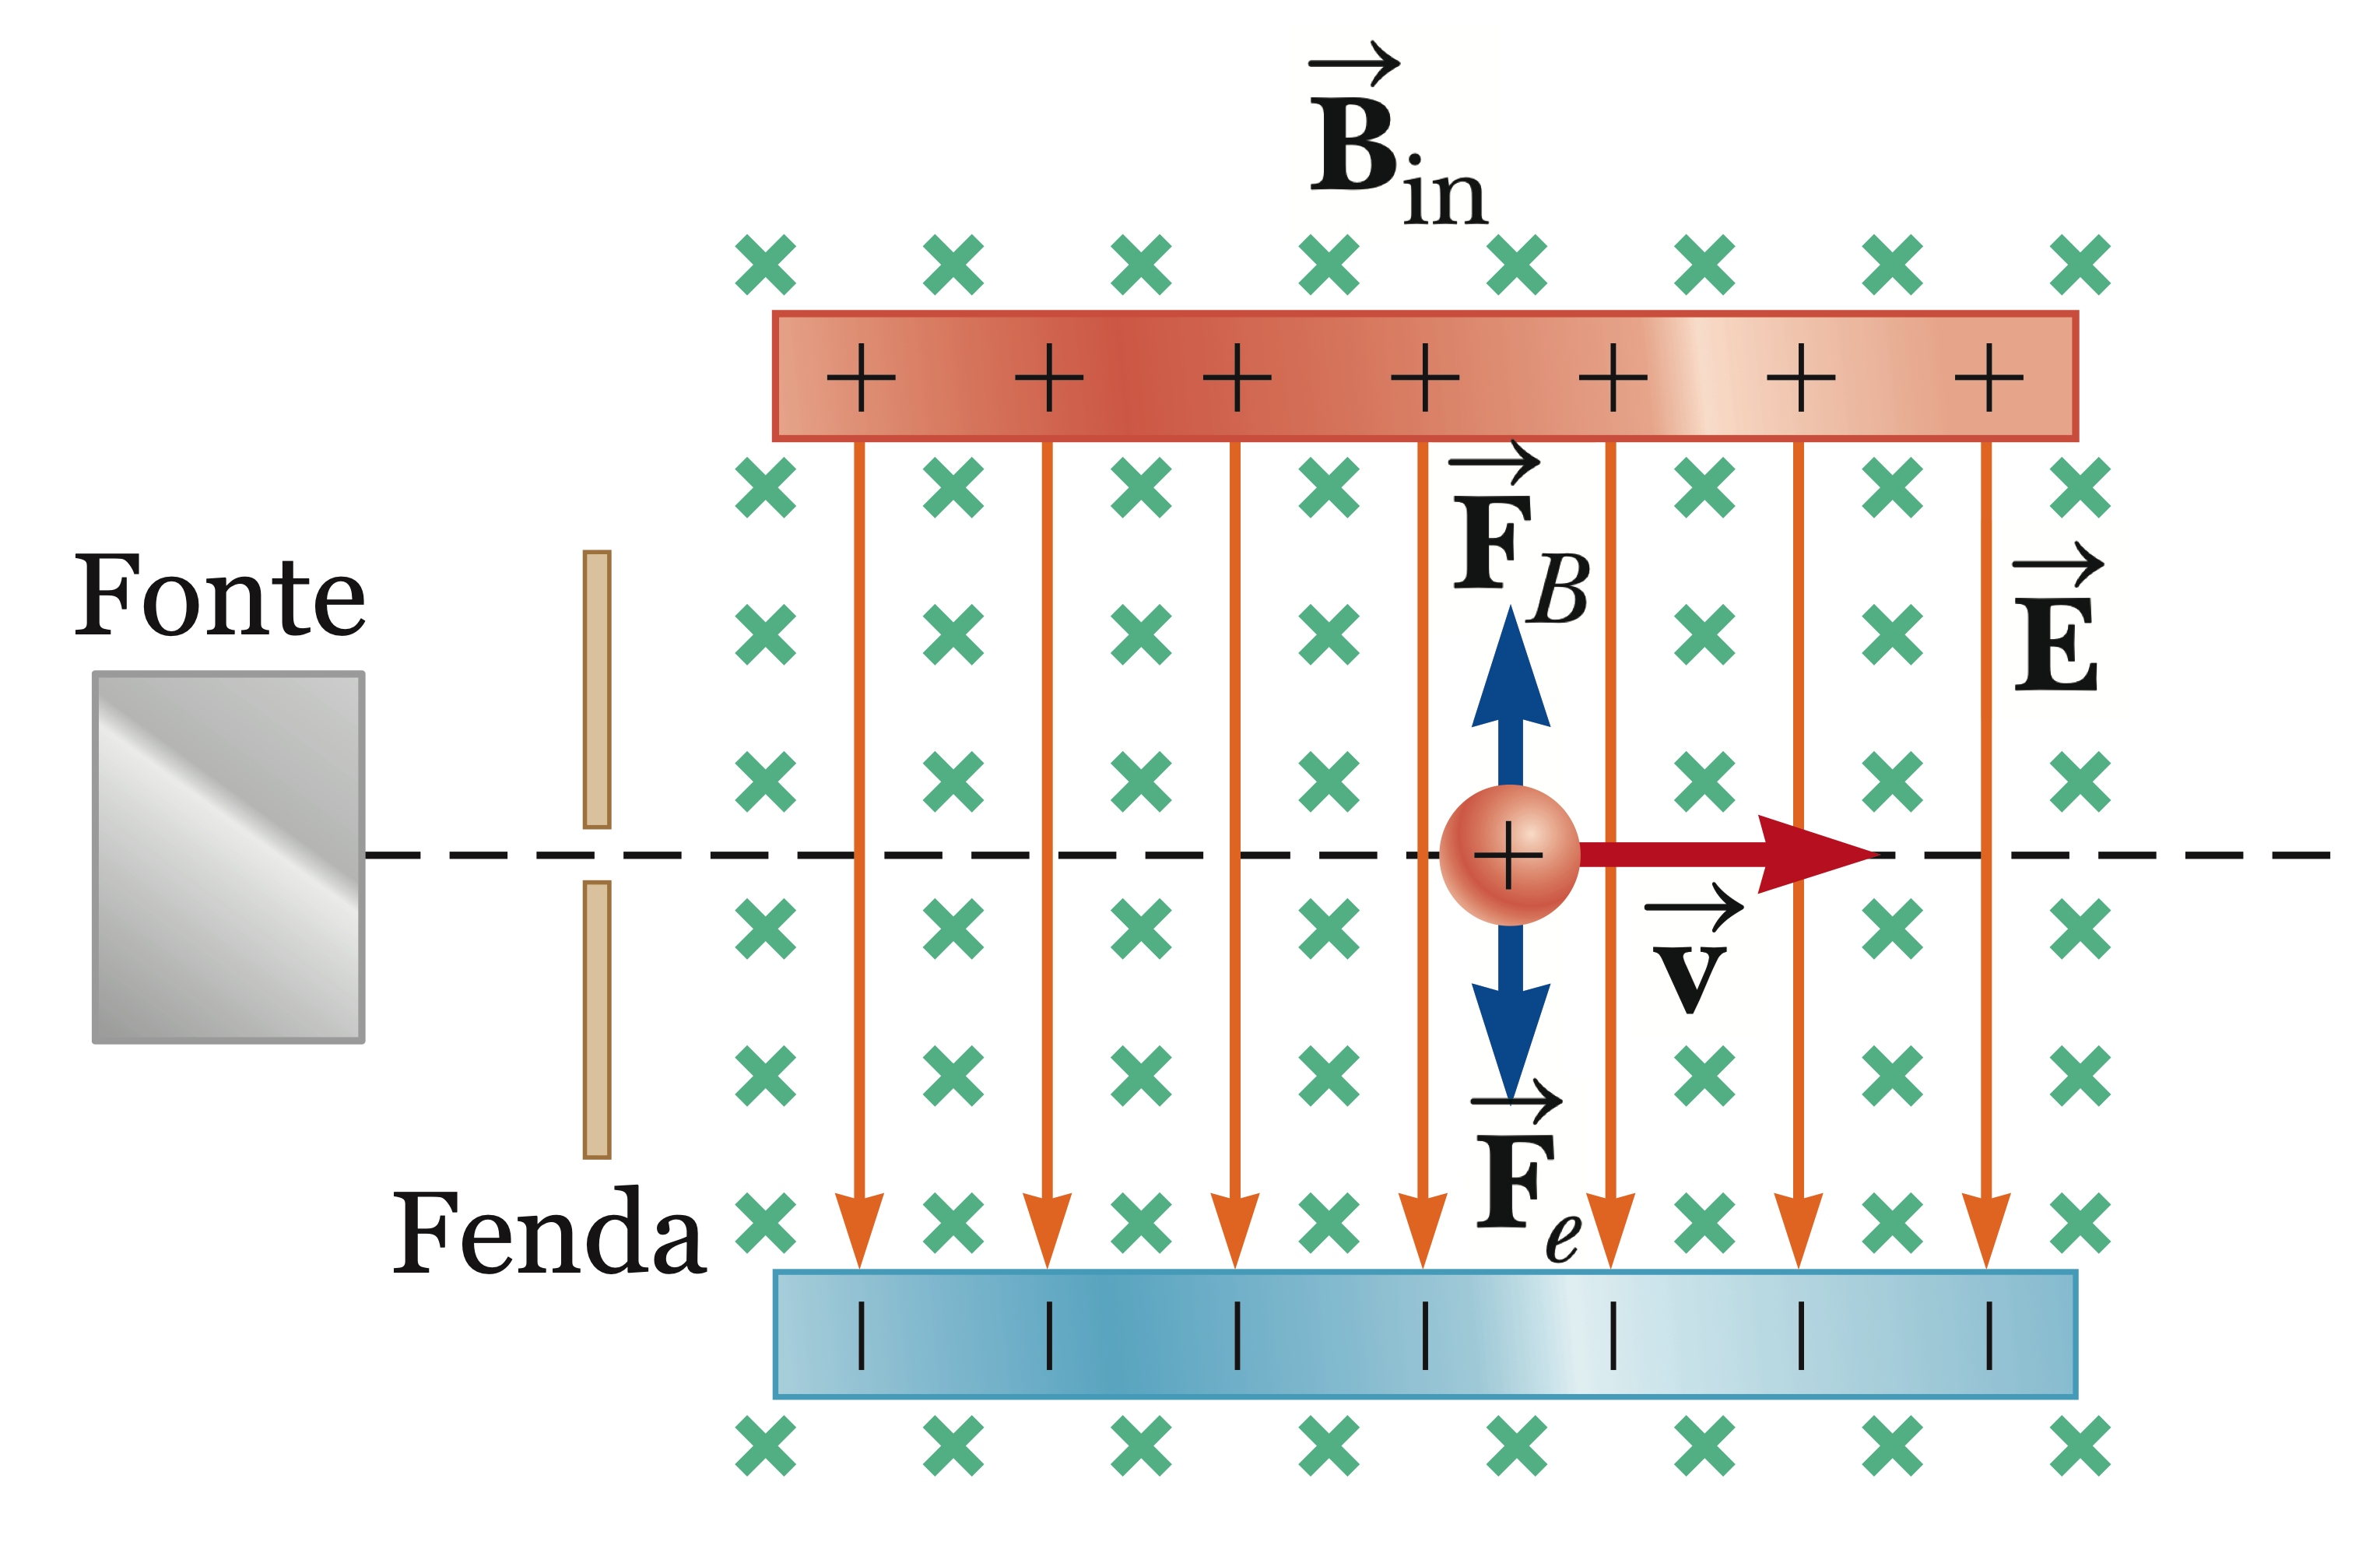
\includegraphics[width=0.5\textwidth]{./Lorentz2.png} 
	\caption{ Carga positiva $q$ com velocidade $\vec{v}$, na presença de um campo magnético $\vec{B}_{in}$ e um campo eléctrico $\vec{E}$. Os três vectores são mutuamente perpendiculares e estão orientados de modo que as forças têm sentidos opostos. \label{fig:lorentz2}} 
\end{figure}

\begin{equation}
m\frac{v^2}{R}=qvB \rightarrow R=\frac{mv}{|q|B}
\end{equation}

Um caso particularmente interessante da força de Lorentz verifica-se quando a velocidade da carga é perpendicular tanto ao campo eléctrico como ao magnético. Nesse caso, as duas forças têm a mesma direcção. Adotando uma configuração como a representada na Fig. \ref{fig:lorentz2}, as forças eléctrica e magnética têm sentidos opostos e podem compensar-se, anulando-se, o que permite que a carga mantenha uma trajectória rectilínea.

Nesta repetição da experiência de Thomson iremos utilizar estes dois princípios para determinar a razão $q/m$. Num primeiro conjunto de medidas, iremos determinar o raio da trajectória de um feixe de raios catódicos na presença de um campo magnético. No segundo conjunto de medidas iremos equilibrar as forças de um campo magnético e um eléctrico de modo a que o feixe tenha uma forma aproximadamente rectilínea.

\newpage
\section{\sf Figuras dos aparelhos da montagem experimental}
\begin{figure}[ht]
	\centering 
	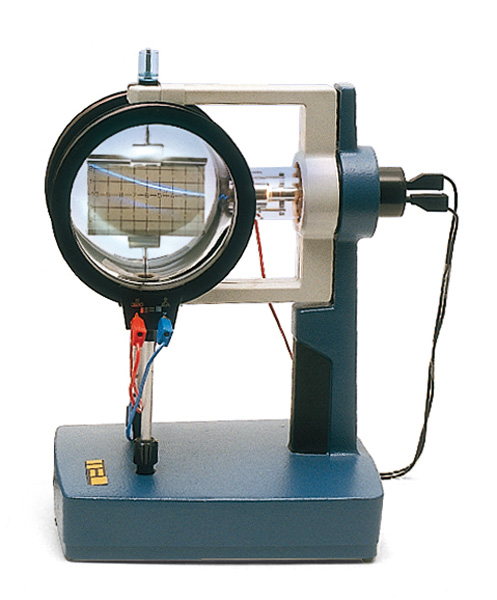
\includegraphics[width=0.45\textwidth]{./fig3-ThomsomEquip}
	\caption{Montagem da Experiência de Thomson com tubo de raios catódicos, suporte e par de bobinas de Helmholtz. \label{fig:Thomson_Equip}} 
\end{figure}

\begin{figure}[hb]
	\centering 
	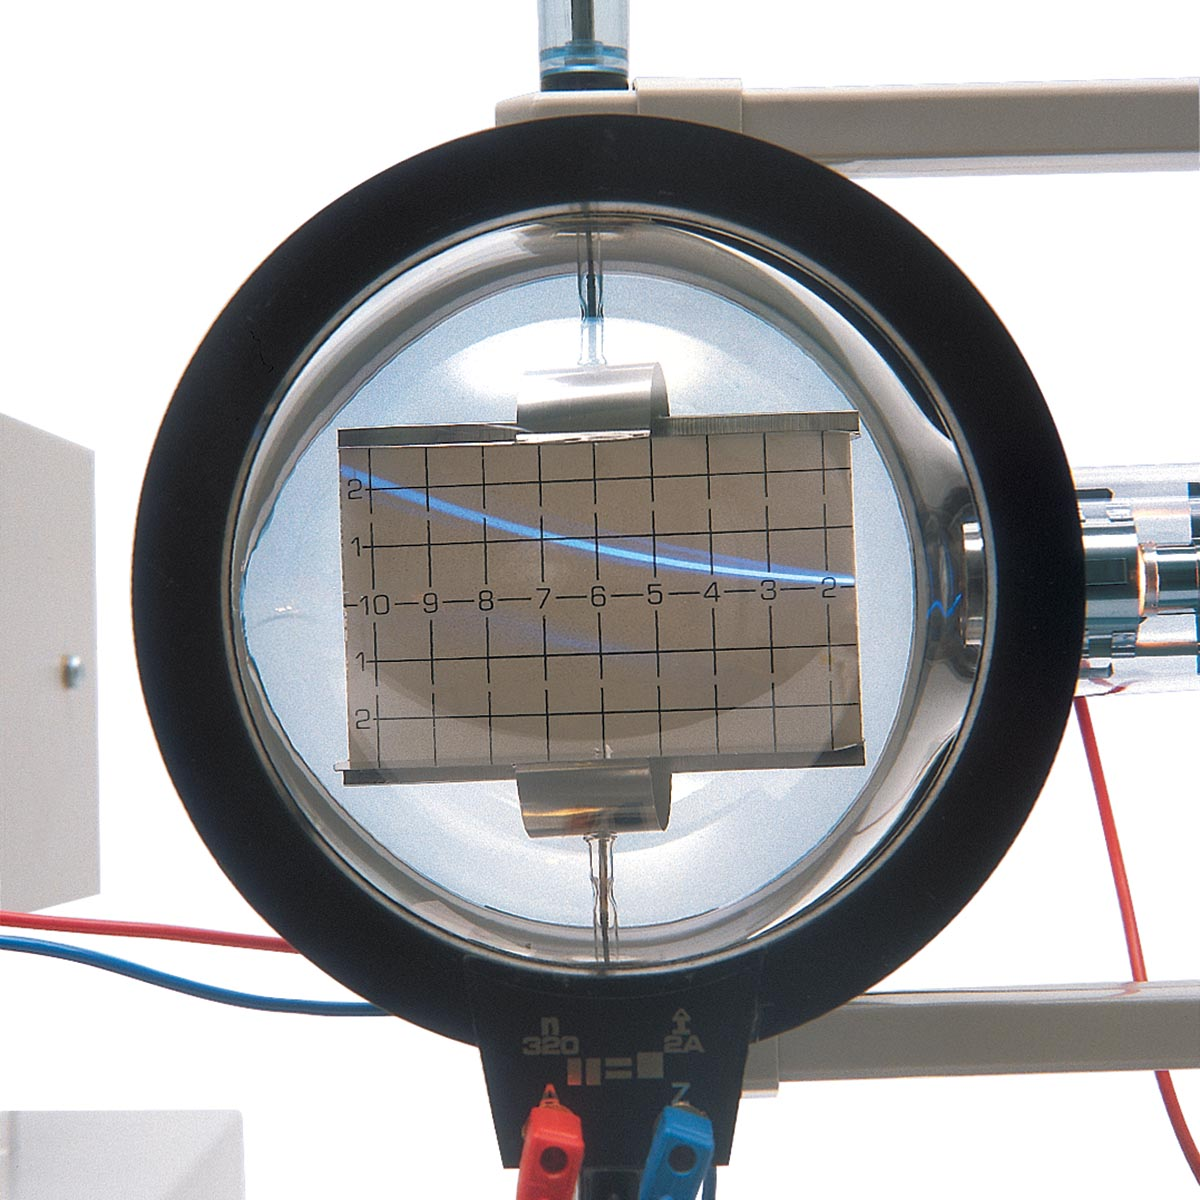
\includegraphics[width=0.4\textwidth]{./fig4-Thomson_Electron-Deflection-Tube-D}
	\caption{Trajectória dos electrões sujeitos a um campo magnético perpendicular. \label{fig:Thomson_trajec}} 
\end{figure}



\newpage

\section{\sf Procedimento Experimental}
\subsection {\sf Material}
\begin{enumerate}
	\item Ampola (tubo) de raios catódicos (TRC), modelo TEL 525.
	\item 	Fonte de alimentação do TRC, que inclui alimentação de alta tensão contínua 
	(até 5000 V) aplicada aos eléctrodos (cátodo e ânodo) do TRC e alimentação de baixa tensão
	(6.3 V AC) para o filamento do TRC.
	\item Par de bobinas que envolvem a parte esférica do TRC na configuração de
	Helmholtz (para criar um campo magnético aproximadamente homogéneo na
	região central entre as bobinas, de raio médio $r$, e afastadas de $r$ uma da outra).
	\item Fonte de alimentação de corrente \textbf{contínua} (em modo DC) para as bobinas.
	\item Multímetro (como amperímetro) a instalar em \textbf{série} no circuito das bobinas.
\end{enumerate}

O tubo TRC tem um filamento alimentado por 6.3 V (em modo AC). Este filamento emite electrões por efeito termiónico. 
Entre o ânodo e o cátodo do tubo estabelecem-se diferenças de potencial $ (V_+ - V_-) = U_a$ . Os electrões são acelerados entre o cátodo e o ânodo e a sua velocidade à saída do ânodo é função de $U_a$. 

Ao entrarem na parte esférica do tubo, os electrões podem ser deflectidos por \emph{campos magnéticos} provocados por correntes que percorrem as bobinas de Helmholtz e/ou por \emph{campos eléctricos} devidos à aplicação de tensão entre duas placas paralelas ligadas aos pontos 1 e 2 do diagrama (Fig. \ref{fig:TL}).

O campo de indução magnética $B$ devido às bobinas de Helmholtz é aproximadamente uniforme na região central entre as bobinas, e para uma corrente $I$ é dado por\footnote{No sistema SI, a unidade de campo magnético é o Tesla (T), sendo 1\,T=1\,Weber/m$^{2}$ .}:
\begin{align}
	\label{eq:helmotz}
	 n &= 320\textrm{ espiras} \nonumber \\ 
B = \left(\frac{4}{5}\right)^{3/2} \cdot \frac{\mu_0 n I}{r} =  \frac{32 \pi n }{5 \sqrt{5}} \cdot \frac{I}{r} \cdot 10^{-7}\textrm{ Weber/m}^{2}
 \qquad  r  &= 0.068\textrm{ m} \\
r  &= d/2 \nonumber
\end{align}

\begin{figure}
	[h]  \centering 
	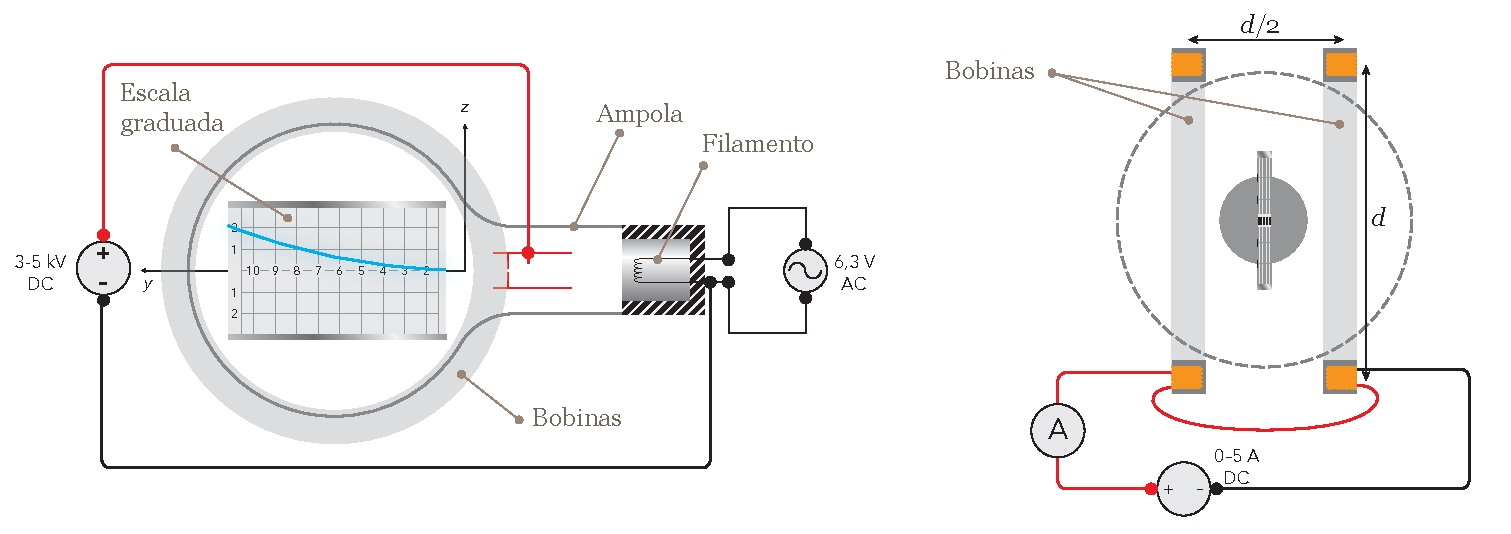
\includegraphics[width=1\textwidth]{fig5-TuboTL.pdf} 
	\caption{Diagrama do tubo utilizado e geometria das bobinas de Helmholtz. Esquerda: vista lateral, com ligações eléctricas do filamento e da tensão de aceleração. Direita: vista frontal, com ligações das bobinas de Helmholtz. \label{fig:TL}} 
\end{figure}

\subsection{\sf Determinação de $q/m$ por deflexão magnética}
\subsubsection{\sf Trajectórias de partículas carregadas sujeitas a um campo magnético constante}
Quando se aplica uma tensão $U_a$ entre o ânodo e o cátodo (sem aplicar tensão entre os pontos 1 e 2 representados na Fig. \ref{fig:TL}), pode admitir-se que a velocidade final $v$ dos electrões ao abandonarem o ânodo é dada pela seguinte expressão 

\begin{equation}
	\label{eq:encin11}
q\, U_a = \frac{1}{2} m \, v^2
\end{equation}
em que $q$  é a carga do electrão e $m$ a sua massa.

Os electrões entram, com velocidade horizontal, na parte esférica do tubo, onde são deflectidos pelo campo magnético $\vec{B}$ (com $\vec{B}\perp\vec{v})$. A sua trajectória passa então a ser circular, com raio $R$, verificando-se:
\begin{equation}
	\label{eq:encin12}
B \, q\, v = \frac{m\,v^2}{R} 
\end{equation}
As trajectórias dos electrões podem ser visualizadas numa escala graduada feita de material fluorescente. 
A origem do reticulado está situada aproximadamente no início da zona 
sujeita ao campo $\vec{B}$.
Combinando (\ref{eq:encin11}) e (\ref{eq:encin12}) obtém-se uma expressão para a relação $q/m$:
\begin{equation}
	\label{eq:encin3}
 \frac{q}{m} = \frac{2\, U_a}{B^2\,R^2} 
\end{equation}
em que:
\begin{description}
\item[$U_a$] – impõe-se e mede-se diretamente no voltímetro da fonte de tensão.
\item[$B$] – calcula-se, para uma dada corrente $I$, a partir da expressão (\ref{eq:helmotz}).
\item[$R$] – determina-se por leitura no écran fluorescente, das coordenadas de posição $y$ (horizontal) e $z$ (vertical) de pontos do feixe. Por construção do tubo verifica-se:
\begin{equation}
	\label{eq:eR}
 R = \frac{y^2 + z^2}{2 \, z} 
\end{equation}
\end{description}



\subsubsection{\sf Modo de proceder}


\begin{enumerate}
	\item Montar os circuitos eléctricos de acordo com a  Fig. \ref{fig:TL}. Note que as ligações das bobinas devem garantir que a corrente eléctrica é percorrida no mesmo sentido, em ambas: para isso, deve usar os conectores na ordem $A\rightarrow Z$ numa bobina e na ordem inversa na outra bobina. Chamar o docente para verificação, \textbf{antes de ligar os aparelhos}.
	\item Verfifique qual é o valor máximo da tensão disponível na fonte de alta tensão. Escolha um valor ligeiramente inferior.
	\item Ajustar a corrente das bobinas de Helmholtz $I_+$ de modo a que a circunferência passe por um ponto bem determinado\footnote{Utilize de preferência os maiores valores possíveis para o raio $R$, de forma a que o feixe se encontre na zona central entre as bobines.}.  Calcule $R$.
	Inverta o sentido da corrente e determine um novo $I_-$ para o mesmo raio $R$.
	Tomando $I_{\textrm{medio}} = (I_+ + I_-)/2 $ calcule o campo magnético $B_{\textrm{medio}}$. Utilize a semi-diferença, $(I_+ - I_-)/2$, para a estimativa das incertezas $\delta I_{\textrm{medio}}$ e $\delta B_{\textrm{medio}}$.
	\item Repita o ponto 2) para quatro novos valores de $R$. 
	\item Repetir 1), 2) e 3)  e para os mesmos $R$, para dois valores inferiores de tensão, afastados por exemplo de 500 V entre si.
	\item Apresente os valores de $q/m$ para os 15 pares de determinações. Calcule a média desses valores, assim como a incerteza da média.
	\item Para um dos pares de pontos, estime a contribuição relativa das incertezas das grandezas que mediu para a incerteza total. Compare este erro assim calculado com a incerteza calculada a partir dos 15 valores calculados.
	Apresente para cada raio o valor de $q/m$ assim como o erro associado a cada uma das determinações. Compare e comente os resultados.
	\item Apresente um valor final para $q/m$. Estime a precisão e a exatidão obtida nas determinações que realizou.
\end{enumerate}
 
\subsection{\sf Determinação de $q/m$ por deflexão magnética e eléctrica quase compensada }

\subsubsection{\sf Situação de equilíbrio entre as interacções eléctrica e magnética}

Se, na força de Lorentz, os dois termos se equilibrarem -- ou seja, se as forças electrostática e magnética forem de igual módulo e de sentidos opostos -- a carga $q$ não é desviada da sua trajectória. No nosso caso, em que $\vec{B} \perp \vec{v}$ , a condição de equilíbrio é dada por:
\begin{equation}
	\label{eq:equil1}
 |\vec{E}| = v\, |\vec{B}|
\end{equation}

\subsubsection{\sf Montagem a efectuar}

Aproveitando a montagem já efectuada no ponto anterior, ligue agora os terminais 1 e 2 (Fig. \ref{fig:TLE}) à fonte de alta tensão que gera a tensão $U_a$, produzindo assim na região do écran fluorescente um campo eléctrico. Fazendo com que as bobinas sejam percorridas por uma corrente com intensidade e  ``sentido'' convenientes, podemos obter uma força de origem magnética anti-paralela à provocada pelo campo $\vec{E}$. 
Deste modo, a trajectória visualizada no écran será aproximadamente retilínea, sendo a condição de equilíbrio dada por:

\begin{equation}
	\label{eq:equil2}
 |\vec{E}| = v\, |\vec{B}| = \frac{U_a}{d}
\end{equation}
onde $d$ é a distância entre as placas do écran fluorescente e $U_a$ a tensão entre as mesmas, que é como se disse igual à tensão de aceleração.

\begin{figure}
	[h]  \centering 
	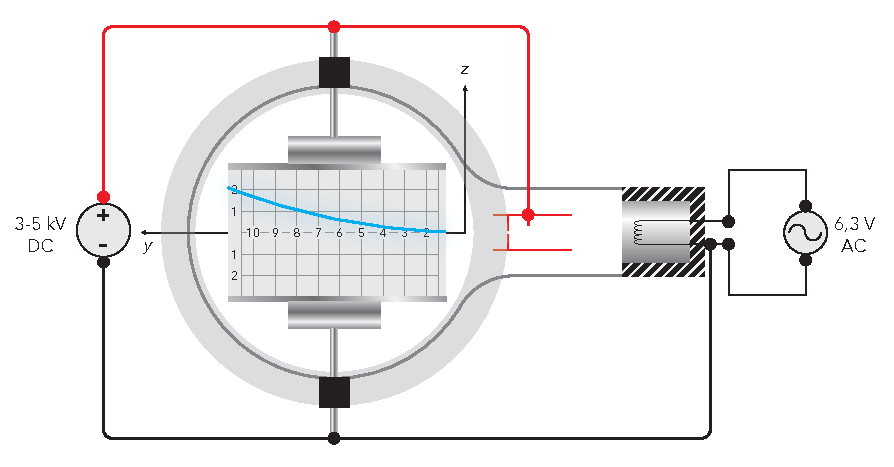
\includegraphics[width=1\textwidth]{fig6-TuboTLE.pdf} 
	\caption{Deflexão magnética e eléctrica quase compensada: ligações eléctricas do filamento, da tensão de aceleração e das placas. \label{fig:TLE}} 
\end{figure}


A equação (\ref{eq:equil2}) permite-nos calcular a velocidade dos electrões, uma vez que podemos conhecer os valores de todas as outras variáveis aí intervenientes. O conhecimento de $v$ permite-nos calcular $q/m$ tendo em conta que, segundo (\ref{eq:encin11}), deverá ser:

\begin{equation*}
\label{eq:encin1}
\frac{q}{m} = \frac{v^2}{2} \; \frac{1}{U_a}
\end{equation*}

Ou finalmente, por combinação com (\ref{eq:equil2}):
\begin{equation}
	\label{eq:qmquase}
\frac{q}{m} = \frac{1}{2} \; \frac{U_a}{B^2\; d^2} 
\end{equation}

\subsubsection{\sf Modo de proceder}
\begin{enumerate}
	\item Para cada uma das quatro tensões de trabalho $U_a$ já referidas, aplicadas agora também às placas que produzem o campo eléctrico, determine o valor de $B$ (a partir de $I$) que conduz ao anulamento das forças de origem eléctrica e magnética.
	\item Inverta o sentido dos campos eléctricos e magnéticos e repita a determinação do valor de $B$.
	\item Apresente os valores de $q/m$. Analise as diferentes contribuições para a incerteza total. Estime o valor da relação carga/massa do electrão, assim como a precisão e a exatidão obtida nas determinações que realizou.
	\item  Observe  a  trajectória  quando  as  forças  de 
origem eléctrica e magnética não se compensam. Comente. 
%	Apresente os valores de q/m calculados assim como o erro associado a cada determinação. Apresente um valor final para $q/m$.
\end{enumerate}

%%%%%%%%%%%%%%%%%%%%%%%%%%%%%%%%%%%%%%%%%%%%%%%%%
%%%%%%%%%%%%%%%%%%%%%%%%%%%%%%%%%%%%%%%%%%%%%%%%%
%%%%%%%%%%%%%%%%%%%%%%%%%%%%%%%%%%%%%%%%%%%%%%%%%
%%%%%%%%%%%%%%%%%%%%%%%%%%%%%%%%%%%%%%%%%%%%%%%%%
%%%%%%%%%%%%%%%%%%%%%%%%%%%%%%%%%%%%%%%%%%%%%%%%%
%%%%%%%%%%%%%%%%%%%%%%%%%%%%%%%%%%%%%%%%%%%%%%%%%
%%%%%%%%%%%%%%%%%%%%%%%%%%%%%%%%%%%%%%%%%%%%%%%%%
%%%%%%%%%%%%%%%%%%%%%%%%%%%%%%%%%%%%%%%%%%%%%%%%%
%%%%%%%%%%%%%%%%%%%%%%%%%%%%%%%%%%%%%%%%%%%%%%%%%
%%%%%%%%%%%%%%%%%%%%%%%%%%%%%%%%%%%%%%%%%%%%%%%%%

%\begin{multicols}{1}
\HRule \\[0.5cm]		
\chapter{\huge{Experiência de Millikan}}
\large {Estimativa da carga eléctrica de gotículas de óleo electrizadas em suspensão num fluido} \\
	\HRule \\%[0.5cm]

\section{\sf Objectivo do trabalho}
Pretende-se com este trabalho determinar a carga eléctrica de pequenas gotas de óleo, tendo como objetivo final mostrar que a carga eléctrica não aparece com uma quantidade qualquer mas sempre como um múltiplo de uma unidade fundamental: a carga do electrão. Deste modo, um corpo electrizado apresenta um excesso de carga de sinal positivo ou negativo, mas cuja valor é sempre um múltiplo do valor da carga elementar $q_{ele}= 1,602176634\cdot 10^{-19}\,$ C.
Traduz-se este facto dizendo-se que a carga eléctrica é \emph{quantizada}.

Dentro das várias experiências elaboradas para mostrar este facto, uma montagem clássica é a do físico americano Robert A. Millikan\footnote{Millikan recebeu o prémio Nobel da Física em 1923 pelos seus trabalhos sobre a determinação da carga do electrão e efeito fotoeléctrico.} (1869-1953), também chamada experiência da gota de óleo.

\section{\sf Conceitos fundamentais}
%\section{\sf }
%\subsection{\sf }
\subsection{\sf Corpo esférico em queda livre num fluido}
Um corpo de dimensões muito pequenas,\footnote{Com número de Reynolds $Re= \frac{\rho v L}{\eta}$ inferior a $\simeq 100$}  ao mover-se com uma velocidade relativamente baixa através de um fluido (líquido ou gás), fica sujeito a uma força de atrito aproximadamente proporcional à sua velocidade, modelada pela expressão:

\begin{equation}
	\label{eq:f_atrito}
	\vec{F}_{at} = - k \, \eta \vec{v}
\end{equation}
em que $\eta$ é o coeficiente de viscosidade do fluido, $\vec{v}$ é a velocidade do corpo e $k$ é um coeficiente que depende da forma do corpo, que no caso deste ser uma esfera de raio $R$ toma o valor (lei de Stokes): 
\begin{equation}
	\label{eq:coef_atrito}
	k = 6 \pi R
\end{equation}


O coeficiente $k$ virá assim expresso em \emph{metro} no Sistema Internacional (SI) e o coeficiente de viscosidade em Pa$\cdot$s (ou N$\cdot$s/m$^2$).
Normalmente a unidade de viscosidade que aparece na literatura é a unidade do sistema C.G.S. (g/cm$\cdot$s) que é designada por Poise (abreviatura P), verificando-se então a equivalência:

\begin{equation*}
	1 \, \mathrm{P} = 0,1\, \mathrm{Pa}\cdot\mathrm{s}
\end{equation*}

Quando um corpo de massa $m$ cai em queda livre sob a ação do seu peso ($\vec{P}=m\vec{g}$) através de um fluido, o seu movimento de queda será abrandado pela força de atrito, e a equação do movimento escreve-se:

\begin{equation}
	\label{eq:mov}
	m\,a \equiv m\, \frac{\ud\, v}{\ud\, t} =  m\,g - k  \, \eta \, v
\end{equation}

A partir de uma velocidade inicial nula, e sendo o peso do corpo constante, a aceleração $a$ produz um aumento  em $v(t)$ e, por consequência, um aumento na força de atrito $F_{at}$. Para uma determinada velocidade limite $v_L$, o segundo membro de (\ref{eq:mov}) anula-se e o corpo passará a deslocar-se com movimento uniforme. A velocidade limite $v_L$ será então obtida fazendo $a= 0$ na equação (\ref{eq:mov}):

\begin{equation}
	\label{eq:vlimit}
	v_L = \frac{m\,g}{k  \, \eta}
\end{equation}
o que poderá ser facilmente constatado pela resolução\footnote{Ver notas de apoio às aulas teóricas} da equação (\ref{eq:mov}), cuja solução é da forma:

\begin{equation}
	\label{eq:vlimita}
	v(t) = \frac{m\,g}{k  \, \eta} (1 - e^{- (k\,\eta / m) t}) = v_L (1-e^{-t/\tau})
\end{equation}
à qual corresponde o gráfico  da Fig~\ref{fig:vLim}, e onde se definiu o tempo característico $\tau=k\eta/m$. Quando $t \to \infty$ temos $v(t) \to v_L = \frac{m\,g}{k  \, \eta} $.


%\end{multicols}

\begin{figure}[tb]
  \centering 
	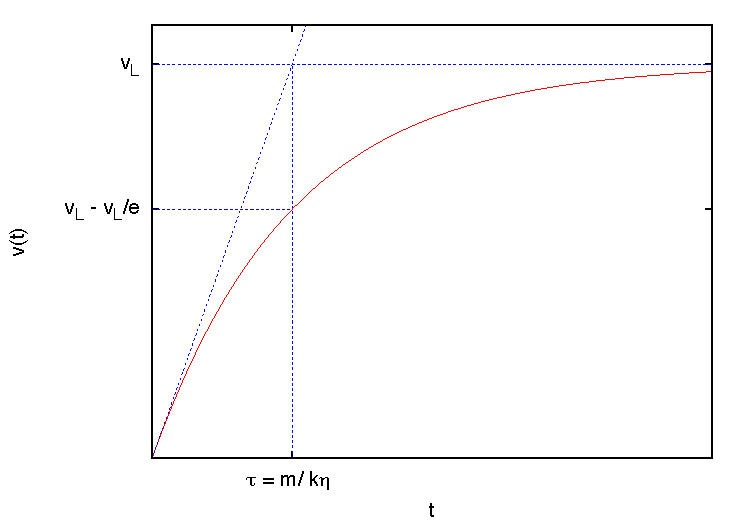
\includegraphics[width=0.6\textwidth]{./plote}
	\caption{ Evolução da velocidade de um corpo em queda livre sujeito a uma força de atrito. \label{fig:vLim}} 
\end{figure}

%\begin{multicols}{2}

Se pretendermos ser mais rigorosos, devemos substituir  em (\ref{eq:vlimit}) o peso do corpo pelo seu “peso aparente” no fluido. De fato, um corpo em queda livre através de um fluido experimenta, além da ação da força de atrito, outra força de baixo para cima cujo módulo é igual ao peso do fluido deslocado pelo corpo, de acordo com o Princípio de Arquimedes. Assim, as equações (\ref{eq:mov}) e (\ref{eq:vlimit}) deverão ser modificadas para:

\begin{equation}
	\label{eq:mov2}
	m\,a = m\,g - m_f\,g  - k  \, \eta \, v
\end{equation}
\begin{equation}
	\label{eq:vlimit2}
	v_L = \frac{(m - m_f)\,g}{k  \, \eta}
\end{equation}
onde $m_f$ é a massa do fluido deslocado. No caso de um corpo esférico de raio $R$, introduzindo a equação (\ref{eq:coef_atrito}) em (\ref{eq:vlimit2}) e atendendo a que:

\begin{equation*}
	m = \frac{4}{3} \pi R^3 \rho \quad \textrm{  e } \quad  m_f = \frac{4}{3} \pi R^3 \rho_f
\end{equation*}
obtemos
\begin{equation}
	\label{eq:vlimit3}
	v_L = \frac{2\,R^2\, (\rho - \rho_f)\,g}{9  \, \eta}
\end{equation}
em que $\rho$  e $\rho_f$ são as massas específicas do corpo e do fluido. Note-se que conhecendo o raio do corpo é pois possível determinar  a sua velocidade limite de queda, e vice-versa.

%

%\end{multicols}

\begin{figure}
	[tb]  \centering 
	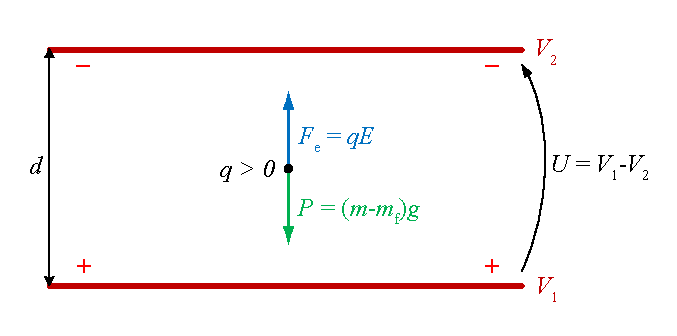
\includegraphics[width=0.7\textwidth]{./F_equil}
	\caption{Equilíbrio de forças numa gota sujeita a campos gravítico e eléctrico. \label{fig:f_equil}} 
\end{figure}

%\begin{multicols}{2}

\subsection{\sf Equilíbrio dum corpo carregado, imerso num fluido, através de um campo eléctrico vertical}

Considere o esquema representado na figura \ref{fig:f_equil}, em que um fluido não condutor se encontra entre duas placas condutoras paralelas separadas de uma distância $d$. Ao aplicar-se uma diferença de potencial \mbox{$U = V_1 -V_2 > 0$} com a polaridade indicada na figura, é criado um campo eléctrico ascendente. Se entre as placas se encontrar uma partícula de massa $m$ e carga positiva\footnote{No caso da partícula estar carregada negativamente obteríamos o mesmo resultado invertendo o sentido do campo eléctrico.} $q$  esta ficará sujeita a uma força eléctrica que contrariará a sua queda.
Na hipótese do campo eléctrico ser uniforme\footnote{Nomeadamente, se a distância entre as placas for muito menor que as suas dimensões laterais.} o módulo de $\vec{E}$ e o módulo da força eléctrica $\vec{F}_e$ que atua na partícula serão dados por:
\begin{equation*}
	E = \frac{U}{d}, \qquad  F_e = |q| \frac{U}{d}
\end{equation*}

Assim, a queda da partícula será agora contrariada pela força eléctrica e pela força de atrito.
A equação (\ref{eq:mov2}) passa a escrever-se:

\begin{equation}
	\label{eq:mov3}
	m\,a = (m - m_f)\,g  - q \frac{U}{d} - k  \, \eta_{ar} \, v
\end{equation}
Variando a diferença de potencial (ddp) $U$, pode-se estabelecer o equilíbrio entre o peso da partícula e a força eléctrica, conseguindo-se a sua paragem entre as placas. Nessa situação, tem-se simultaneamente $F_{at}=0$, $a=0$ e  $v$  $=0$:

\begin{equation}
	\label{eq:equil}
	0 = (m - m_f)\,g  - q \frac{U}{d} 
\end{equation}
Nesta equação a expressão $(m - m_f)\,g$ pode ser substituída usando a equação (\ref{eq:vlimit2}), obtendo-se:

\begin{equation*}
	v_L\, k\, \eta_{ar} = q \frac{U}{d}
\end{equation*}
E entrando também com a eq. (\ref{eq:coef_atrito}) no caso de a partícula ser esférica, obtemos por fim:

\begin{equation}
	\label{eq:carga}
	q = \frac{6 \pi \, R \, \eta_{ar} \, d\, v_L}{U}  
\end{equation}
onde

\begin{itemize}
\item $v_L$, a velocidade limite de queda da partícula através do fluido, na ausência do campo eléctrico
\item $\eta_{ar} = 18,52 \cdot 10^{-5}$ P$ =  18,52 \cdot 10^{-6} \;$ Pa$\cdot$s (viscosidade do ar a 23 $^{\circ}$C)
\item $\rho = 973 \,$ kg/m$^{3}$ (massa específica do óleo de silicone)
\item $\rho_f = 1 \,$ kg/m$^{3}$ (massa específica do ar)
\item $g=9,80\,$ m/s$^{2}$ (aceleração gravítica em Lisboa)
\item $d$ (distância entre placas, a medir no laboratório)
\end{itemize}

\subsection{\sf Correções}
\subsubsection{\sf Temperatura ambiente}

No caso da temperatura ambiente se afastar muito de $23\,^{\circ}\mathrm{C}$, o valor  da viscosidade do ar terá de ser corrigido.\footnote{Utilize por exemplo a calculadora \emph{online}: http://www.lmnoeng.com/Flow/GasViscosity.htm}

\subsubsection{\sf Dimensão das gotas}

A Lei de Stokes não é exata quando as dimensões dos corpos esféricos forem comparáveis à distância média entre as moléculas do ar. Nestas condições, Millikan verificou que a viscosidade $\eta_{ar}$ deveria ser substituída por:

\begin{equation}
	\label{eq:correcao}
	\eta_{ar}' = \frac{\eta_{ar}}{1 + b/(p\,R)}  
\end{equation}
em que a constante $b=7,88\cdot 10^{-3}$ Pa$\cdot$m, 
$p$ é pressão atmosférica expressa em pascal e $R$ é o raio da gota em metros.
%$0.000617$, $p$ é pressão expressa em $cm$ de %mercúrio\footnote{$1\,atm  = 1.013 \times 10^5 \,Pa = %1013 \, mbar %= 76\, cm_{Hg}$}  e $R$ é o raio da gota em %$cm$.

O valor corrigido $q'$ será  determinado a partir do valor experimental $q$ por

\begin{equation}
	\label{eq:correcao1}
	q' = q\, \left(\frac{\eta_{ar}'}{\eta_{ar}}\right)^{3/2}  =q\, \left(\frac{1}{1 + b/(p\,R)}\right)^{3/2}  
\end{equation}

\section{\sf Figuras dos aparelhos da montagem experimental}
\begin{figure}
	[htb]  \centering 
	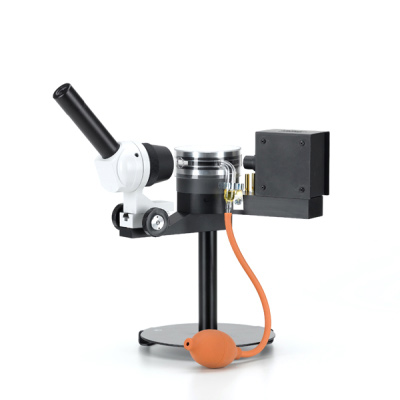
\includegraphics[width=0.5\textwidth]{./U131001_01_Aparelho-de-Millikan}
	\caption{Equipamento para determinação da carga das gotas. \label{fig:Equi}} 
\end{figure}

\begin{figure}
	[htb]  \centering 
	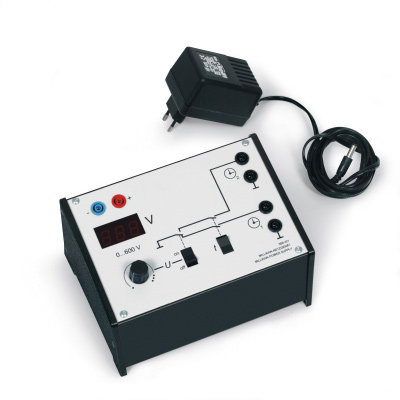
\includegraphics[width=0.5\textwidth]{./U13105-230_01_Aparelho-operacional-de-Millikan}
	\caption{Gerador de alta tensão DC regulável. \label{fig:fonteDC_HT}} 
\end{figure}


\newpage
\section{\sf Procedimento experimental}


\subsection{\sf Material}

\begin{enumerate}
	\item Célula de Millikan com gerador de alta tensão DC regulável
	\item  Atomizador e óleo de silicone
	\item Cronómetro
	\item Nível de bolha de ar% Parafuso para calibração do retículo do microscópio
\end{enumerate}


\subsection{\sf Trabalho preparatório} 
\begin{enumerate}
\item Preencha os objectivos do trabalho que irá realizar na sessão de laboratório. 
\item Preencha o quadro com as equações necessárias para o cálculo das grandezas, bem como as suas incertezas. 
\end{enumerate}

\subsection{\sf Montagem experimental}
Efectue a montagem de acordo com a Fig. \ref{fig:esquema-millikan}. Chame o professor antes de ligar os aparelhos à corrente eléctrica.

\begin{figure}
	[htb]  \centering 
	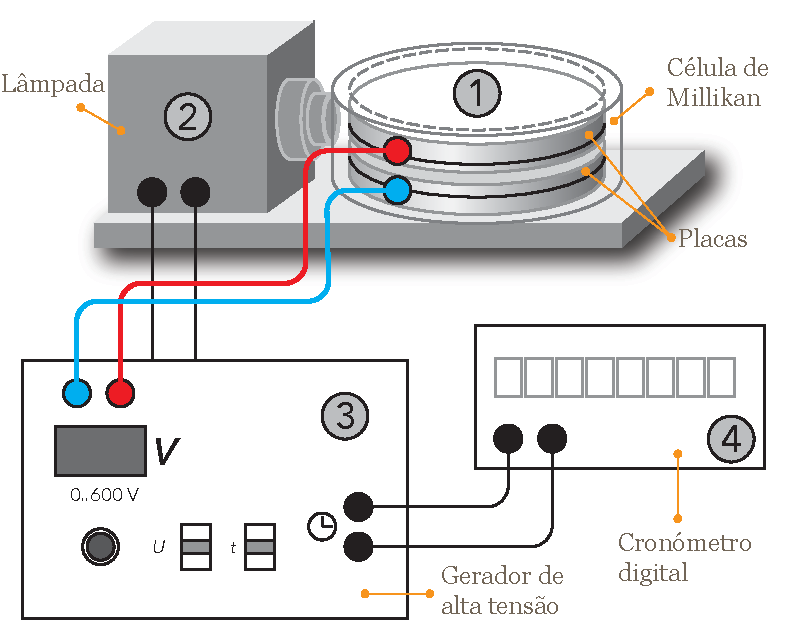
\includegraphics[width=0.6\textwidth]{Esquema-Millikan.pdf}
	\caption{Esquema da montagem da experiência de Millikan. 1 - Célula de Millikan; 2 - lâmpada; 3 - gerador de alta tensão regulável; 4 - cronómetro.\label{fig:esquema-millikan}} 
\end{figure}



\subsection{\sf Determinação da tensão de equilíbrio}
\begin{enumerate}
\item   Depois de verificar que a célula está horizontal, meça o distância entre placas, $d$. Tente focar o microscópio na zona onde as gotas irão ``flutuar''. Atenção: o microscópio amplia a imagem e a escala por 2$\times$.

\item Coloque o potenciómetro que controla a alimentação das placas do condensador no valor mínimo de tensão eléctrica. 

\item    Verifique se o interruptor de inversão da alimentação do condensador está na posição ``Neutra''. Rode o potenciómetro para uma posição que permita, quando ligar o interruptor de inversão, estabelecer um campo eléctrico entre as placas do condensador. 

\item     Utilizando o pulverizador junto do orifício da célula, produza uma pequena ``nuvem'' de gotículas de óleo. Observe através do microscópio o movimento das gotículas em frente do retículo, ajustando a focagem se necessário.

\item     Ligando o interruptor e variando a intensidade  e o  sentido do campo eléctrico, verifique se existem gotículas eletrizadas. 

 \item Escolha uma das gotas e, ajustando a tensão, manipule a sua posição vertical de modo a que esta fique colocada numa determinada divisão do topo do retículo, imobilizando-a de seguida. Registe o valor da tensão. 
 \end{enumerate}
 
 \subsection{\sf Determinação da velocidade limite e da carga}
 \begin{enumerate}
 \setcounter{enumi}{6}

\item Anule o campo eléctrico  e verifique que a gota cai sob acção da gravidade (com velocidade limite). 
Com um cronómetro, meça o tempo necessário para que a gota percorra  $N>4$ divisões
do retículo. 
\item Repondo o campo eléctrico, conduza a gota para a posição inicial para  medir o tempo pelo menos duas vezes. 

\item Troque de posição com o colega para repetir este processo para várias gotas, tentando escolher as gotas de menor carga.

\item   Para cada gota, calcule a velocidade limite média e a respectiva incerteza, usando esse valor para estimar o raio e 
a carga. Calcule a carga corrigida pela viscosidade.

\item De modo a obter resultados mais fiáveis, tente assegurar-se de que as diversas gotas apresentam valores experimentais diferentes. Duas gotas com valores da velocidade limite e raio muito semelhantes têm provavelmente a mesma carga, pelo que deverá repetir as medições para uma gota diferente.
\end{enumerate}

\subsection{\sf Análise, conclusões e comentários finais}
Discuta a qualidade dos dados obtidos e as conclusões que pode retirar desta experiência. Comente também sobre as condições de realização da experiência, dos equipamentos utilizados e a influência de erros aleatórios e sistemáticos, identificando-os. Supondo que não conhecia o valor tabelado da carga do electrão, e apenas a partir dos resultados obtidos, poderá tirar conclusões sobre a quantificação da carga eléctrica?\\
\HRule \\[0.5cm]

%\end{multicols}


%%%%%%%%%%%%%%%%%%%%%%%%%%%%%%%%%%%%%%%%%%%%%%%%%
%%%%%%%%%%%%%%%%%%%%%%%%%%%%%%%%%%%%%%%%%%%%%%%%%
%%%%%%%%%%%%%%%%%%%%%%%%%%%%%%%%%%%%%%%%%%%%%%%%%
%%%%%%%%%%%%%%%%%%%%%%%%%%%%%%%%%%%%%%%%%%%%%%%%%
%%%%%%%%%%%%%%%%%%%%%%%%%%%%%%%%%%%%%%%%%%%%%%%%%
%%%%%%%%%%%%%%%%%%%%%%%%%%%%%%%%%%%%%%%%%%%%%%%%%
%%%%%%%%%%%%%%%%%%%%%%%%%%%%%%%%%%%%%%%%%%%%%%%%%
%%%%%%%%%%%%%%%%%%%%%%%%%%%%%%%%%%%%%%%%%%%%%%%%%
%%%%%%%%%%%%%%%%%%%%%%%%%%%%%%%%%%%%%%%%%%%%%%%%%
%%%%%%%%%%%%%%%%%%%%%%%%%%%%%%%%%%%%%%%%%%%%%%%%%

	
\chapter{\huge{Velocidade da luz}}
\large {\bf {Determinação para diferentes materiais homogéneos e isotrópicos}}\\
	\HRule \\%[0.5cm]

\section{\sf Objectivo do trabalho}
\begin{itemize}
\item Medição da velocidade da luz em diferentes meios homogéneos e isotrópicos: ar, vidro acrílico, água.
\item Medição do índice de refracção dos mesmos materiais.
\end{itemize}

\section{\sf Conceitos fundamentais}
Em muitas das experiências descritas na literatura para determinacão da velocidade da luz foram utilizados feixes luminosos pulsados (ou modulados), que percorrem determinados trajetos de maior ou menor comprimento (ver exemplo na Fig. \ref{fig:Fizeau}). 
No presente trabalho, utiliza-se como fonte luminosa um díodo (LED) que emite radiação  visível com um comprimento de onda (c.d.o.) na zona do vermelho. A tensão de alimentação do díodo é sinusoidal de frequência $f_{\textrm{mod}}=50$ MHz, fazendo com que a intensidade da luz emitida $I_{\textrm{diodo}}(t)$ seja \emph{modulada em amplitude} (AM, do inglês \emph{amplitude modulation}), variando entre 0 e $I_0$ de acordo com a expressão

\begin{equation*}
	\label{eq:f_am}
		I_{\textrm{diodo}}(t) = \frac{1}{2}I_0 [1+ \sin ( 2\pi f_{\textrm{mod}} t)]
\end{equation*}
%A(t) \cdot \sin ( 2\pi \cdot f_{luz} \, t) = \underbrace{

\begin{figure}
	[ht!b]  \centering 
	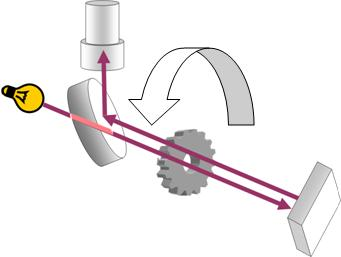
\includegraphics[width=0.35\textwidth]{Fizeau}
	\caption{Esquema do aparelho (Roda de Fizeau) para determinar a velocidade da luz utilizado por Fizeau em 1849. \label{fig:Fizeau}} 
\end{figure}

%\section{\sf Introdução}

\newpage
\subsection{\sf Base do método}
No presente trabalho, o feixe luminoso proveniente do LED emissor é forçado a percorrer um determinado trajeto de comprimento $L$, sendo em seguida a sua intensidade  detectada por um fotodíodo receptor (Fig. \ref{fig:Montagem}). Um par de espelhos colocados a 90$^\circ$ pode deslocar-se ao longo de uma calha, sendo assim possível variar o comprimento do trajeto. Os sinais de amplitude impostos ao emissor e captados no receptor são registados\footnote{Depois de uma deteção \emph{heteródina}, em que a frequência modulada é desviada de \\ 
$f_{\textrm{bat}}=$50.050 MHz -- 50 MHz  = 50 kHz. Esta operação permite a utilização de um osciloscópio simples de banda de frequências mais estreita.} 
nos canais de um osciloscópio funcionando em modo “XY” (sem base de tempo).

\begin{figure}[htb] 
 \centering 
	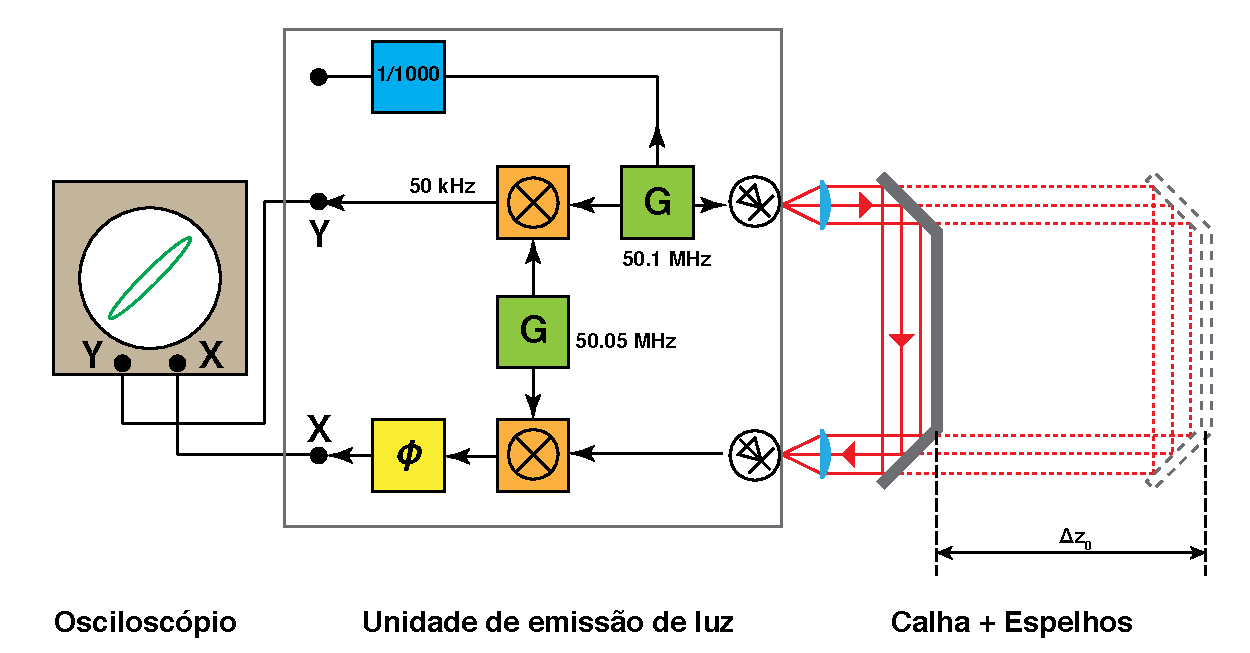
\includegraphics[width=01.0\textwidth]{esquema}
	\caption{Montagem para determinação da velocidade da luz. \label{fig:Montagem}} 
\end{figure}



Em ambos os canais X e Y (vertical e horizontal) a frequência é a mesma\footnote{Os sinais são \emph{coerentes}, pois provêm da mesma fonte.}. No caso mais geral em que os sinais não estão em fase um com o outro, o padrão visualizado no osciloscópio é uma \emph{figura de Lissajous}, neste caso uma elipse (Fig. \ref{fig:fase}), com um parâmetro $\delta$ dado pela equação geral:
\begin{equation}
	\label{eq:elipse}
	\sin^2 \delta = \frac{A_x^2}{A_{x0}^2} + \frac{A_y^2}{A_{y0}^2} - \frac{2 A_y\,A_x}{A_{y0}\,A_{x0}} \cos  \delta
\end{equation}
sendo $A_x(t)$ o sinal de intensidade captado no emissor,  $A_y(t)$ o sinal
proveniente do recetor, $A_{x0}$, $A_{y0}$ as respectivas amplitudes e $\delta$ a desfasagem entre os dois sinais. A desfasagem relativa entre os sinais (e, logo, o ângulo $\delta$) varia com o comprimento do trajecto $L$ percorrido pelo raio luminoso. Este efeito traduz-se numa variação da forma da elipse observada.  A elipse pode degenerar em retas quando os dois sinais estiverem em fase, $\delta = 2n\pi$ (nos quadrantes ímpares)  ou em oposição de fase, $\delta = (2n+1)\,\pi$ (nos quadrantes pares). 

\begin{figure}
	[htb]  \centering 
	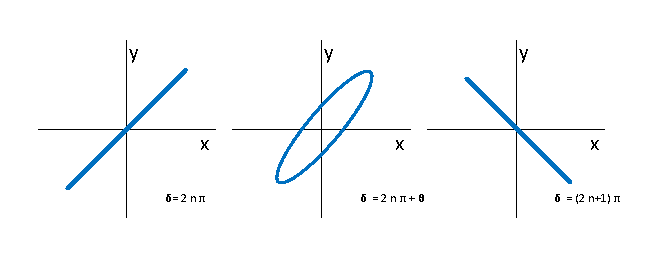
\includegraphics[width=0.8\textwidth]{osci_fase}
	\caption{Figuras de Lissajous observadas no osciloscópio. À esquerda: sinais em fase; centro: sinais com uma dada desfasagem $\theta$; direita: sinais em oposição de fase.  \label{fig:fase}} 
\end{figure}

\subsection{\sf Velocidade da luz no ar}
Neste trabalho, a velocidade da luz é calculada a partir da determinação do comprimento do
caminho suplementar $\Delta L= 2\,\Delta z_0$ (ver Fig. \ref{fig:Montagem}) que a luz tem de percorrer para que se passe de um extremo em que os sinais estão em fase ao extremo oposto de oposição de fase (ou vice-versa). Por definição, para passar de uma situação à outra é necessário que o tempo gasto no percurso suplementar corresponda a metade de um período. Assim, a luz percorre essa distância num intervalo de tempo $\Delta t$ igual a metade do período do sinal modulante, ou seja $\Delta t=T/2=1/(2\cdot50\,\textrm{MHz})= 10\,\textrm{ns}$. 
No trajecto da luz no ar teremos a seguinte expressão para a sua velocidade:
\begin{equation}
	\label{eq:vc}
	c_{ar} = \frac{\Delta L}{\Delta t}=\frac{2\,\Delta z_0}{T/2} 
\end{equation}


\subsection{\sf Velocidade da luz em meios sólidos e líquidos}
 O índice de refração de um meio material $1$ em relação a outro meio $0$, para um dado comprimento de onda, é definido\footnote{Esta definição só é válida se as condutividades eléctricas dos meios $0$ e $1$ forem nulas, ou seja, nos \emph{dieléctricos} perfeitos.}
 como o quociente entre as velocidades de propagação da luz nos meios $0$ e $1$:

 \begin{equation}
	\label{eq:index}
	n_1 \equiv \frac{c_0}{c_1}  = \frac{\frac{1}{\sqrt{\varepsilon_0 \, \mu_0}} }{\frac{1}{\sqrt{\varepsilon_1 \, \mu_1}} } =
		\sqrt{\frac{\varepsilon_1 \, \mu_1}{\varepsilon_0 \, \mu_0}} = \sqrt{\varepsilon_r \, \mu_r}
\end{equation}

Nesta expressão $\varepsilon_0$, $\varepsilon_1$ ,	 $\mu_0$, $\mu_1$ são as constantes dieléctricas e as permeabilidades magnéticas respetivamente do meios $0$ e $1$ e $\varepsilon_r$, $\mu_r$    as relativas $(\varepsilon_1= \varepsilon_r\, \varepsilon_0)$.

\begin{figure}[h!tb]  
	\centering 
	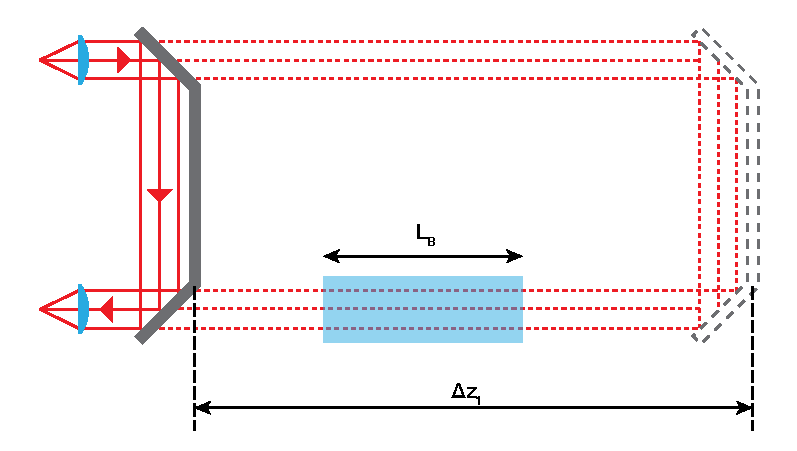
\includegraphics[width=0.8\textwidth]{esquema2}
	\caption{Montagem para determinar índices de refração em sólidos e líquidos. \label{fig:Montagem_bloco}} 
\end{figure}

Se no percurso do feixe luminoso interpusermos um bloco transparente de material sólido ou líquido de comprimento $l_B$ (Fig. \ref{fig:Montagem_bloco}), o comprimento suplementar necessário $\Delta L$ entre as posições de fase e oposição de fase vai variar. De facto, uma vez que as velocidades da luz nesse material e no ar são diferentes, a desfasagem introduzida por uma dada espessura de material também difere da desfasagem causada pela mesma espessura de ar. É pois necessário contabilizar em separado os tempos necessários para percorrer 
\begin{itemize}
\item o bloco de espessura $l_B$ à velocidade $c_B$
\item o restante comprimento $(2\Delta z_1-l_B)$ no ar à velocidade $c_{ar}$
\end{itemize}

Obtém-se assim a expressão

\begin{equation}
	\label{eq:vc_bloco}
	{T/2}  = \frac{2\,\Delta z_1 - l_B}{c_{ar}}  +  \frac{l_B}{c_{B}}
\end{equation}
em que $\Delta z_1$ é a nova posição em que se regista passagem de fase para oposição de fase (ou vice-versa). A partir daqui calcula-se a velocidade $c_{B}$.  

Pode ainda obter-se o valor do índice de refração $n_{B}$ com a ajuda de (\ref{eq:vc}) e (\ref{eq:index}):

\begin{align}
	\label{eq:n_bloco}
	{T/2}  = \frac{2\,\Delta z_0}{c_{ar}}  &=  \frac{2\,\Delta z_1 }{c_{ar}} -   \frac{l_B}{c_{ar}}  +  \frac{l_B}{c_{B}} \nonumber \\ 
	\frac{2\,(\Delta z_0- \Delta z_1 )}{c_{ar}}  &= -   \frac{l_B}{c_{ar}}  +  \frac{l_B}{c_{B}} \nonumber \\
	\frac{2\,(\Delta z_0- \Delta z_1 )}{l_B} &= -1 +  \frac{c_{ar}}{c_{B}} \nonumber \\
	n_{B} &= 1 +  \frac{2\,(\Delta z_0- \Delta z_1 )}{l_B} 
\end{align}

Neste trabalho, serão  determinados os índices de refração e a velocidade da luz em  dois meios materiais: a resina acrílica e a água. 
 


\newpage
\section{\sf Procedimento experimental}
\subsection{\sf Material}

\begin{enumerate}
\setlength{\itemsep}{0mm}
\item Unidade de emissão (com amplitude modulada por um sinal de frequência 50 MHz) e de recepção de luz.
% (díodos receptor) amplitude modulada por um sinal de frequência $50\,MHz$)(.
\item Duas lentes plano-esféricas em suportes de tipo poste, ajustáveis
\item Suporte móvel com dois espelhos planos para inversão do sentido de propagação da luz.
\item Calha de aço inox.
\item Banco óptico de altura ajustável.  
\item Bloco de vidro acrílico transparente.
\item Dois tubos com cerca de 1 metro de comprimento para conter água ou ar. 
\item Osciloscópio de dois canais a funcionar em modo XY.
\end{enumerate}

\subsection{\sf Trabalho preparatório} 
\begin{enumerate}
\item Preencha os objectivos do trabalho que irá realizar na sessão de laboratório. 
\item Preencha o quadro com as equações necessárias para o cálculo das grandezas, bem como as suas incertezas. 
\end{enumerate}


\subsection{\sf Regulação da montagem}
 
 \begin{figure}[h!tb]  
	\centering 
	\includegraphics[width=0.6\textwidth]{Fig5}
	\caption{Posicionamento das lentes no suporte da unidade de emissão de luz. \label{fig:lentes}} 
\end{figure}

\begin{enumerate}
\setlength{\itemsep}{0mm}
\item Comece por efectuar o alinhamento óptico do sistema. Ligue a unidade e posicione a lente junto ao LED emissor. Usando um alvo difusor (papel vegetal, por exemplo), observe a forma da mancha luminosa ao longo do percurso óptico, Ajuste a lente de modo a obter um diâmetro constante (feixe de raios paralelos, ou colimado) e à mesma altura relativamente à mesa. Note que pode ajustar a altura da lente, a sua posição transversal e a distância ao LED.
\item Instale o conjunto de espelhos, assegurando-se de que o feixe incide em ambas as superfícies espelhadas (se for necessário, ajuste de novo a primeira lente, mas sem perder a forma do feixe que obteve). O suporte e os espelhos estão pré-alinhados, pelo que não deverá necessitar de ajustar os seus suportes. Verifique que os espelhos enviam o feixe de volta correctamente. Ainda sem a segunda lente, verifique que a mancha luminosa está centrada com  a janela do díodo receptor. Se não estiver, ajuste a primeira lente (e não os espelhos).
\item Coloque agora a lente no lado do díodo receptor e, ajustando-a, alinhe o foco do feixe convergente de modo a incidir no centro do díodo (ver figura \ref{fig:lentes}).
\item Ligue o osciloscópio às saídas da unidade emissora e visualize ambos os canais (modo DUAL). Optimize a posição da lente no díodo receptor de modo a maximizar a amplitude do \emph{sinal recebido}. Quando tiver terminado, volte a colocar o osciloscópio em mode XY e ajuste de modo a visualizar uma figura de Lissajous contida no écran.
\item Coloque os espelhos na posição zero (posição $z_{\delta=0}$) da escala -- por exemplo, encostando o suporte dos espelhos ao suporte da unidade emissora. Rodando o botão da unidade que ajusta electronicamente a diferença de fase entre os dois sinais, obtenha uma reta dos quadrantes (ím)pares.
\end{enumerate}
 \begin{figure}[h!tb]  
	\centering 
	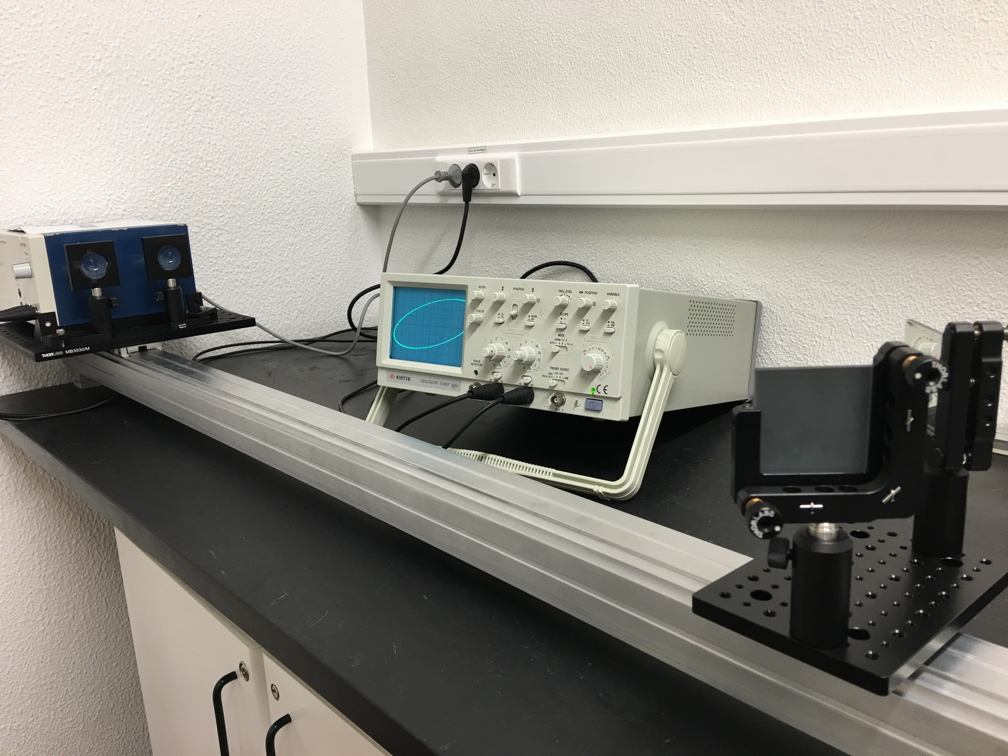
\includegraphics[width=0.6\textwidth]{fig6}
	\caption{Montagem para medição da velocidade da luz no ar. \label{fig:ar}} 
\end{figure}

\subsection{\sf Medição da velocidade de propagação da luz no ar}
\begin{enumerate}
\item Desloque os espelhos sobre a calha e observe a modificação da figura no ecrã do 
osciloscópio, em particular nas posições que correspondem a que os sinais recebidos estejam 
em quadratura $(\delta=\pi/2)$ e oposição de fase $(\delta=\pi)$. Para esta última situação, registe a 
nova posição $z_{\delta=\pi}$ dos espelhos e o intervalo de incerteza entre o qual os sinais parecem estar ainda em 
oposição de fase (ver figura \ref{fig:ar}).
\item Repita o procedimento para cada observador. 
\item Calcule a velocidade de propagação da luz no ar $c_{ar}$, a sua incerteza e o desvio à exatidão\footnote{O valor $c_{ar}$ é muito próximo de $c_{vacuo}$ = 299 792 458 m/s, que é uma constante exacta do Sistema Internacional de Medidas. O índice de refração do ar para a luz visível é $n_{ar}=1.000293$.}. 
\end{enumerate}

 \begin{figure}[h!tb]  
	\centering 
	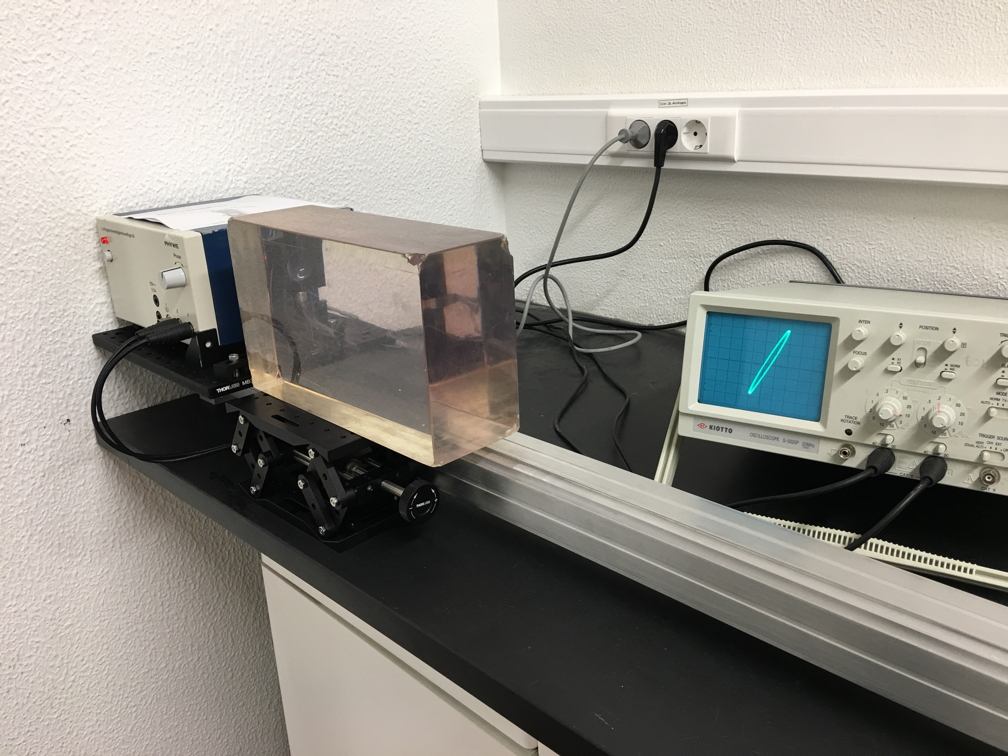
\includegraphics[width=0.6\textwidth]{fig7}
	\caption{Montagem para medição da velocidade da luz no vidro acrílico. \label{fig:vidro}} 
\end{figure}

\subsection{\sf Medição da velocidade de propagação da luz no vidro acrílico}
\begin{enumerate}
\item Verifique novamente se no zero da posição dos espelhos os sinais estão em fase. Usando o banco óptico, ajuste a altura e coloque cuidadosamente o bloco de vidro acrílico no percurso do feixe incidente, de modo a que incida perpendicularmente à face e usando o percurso mais longo no vidro acrílico (figura \ref{fig:vidro})
\item Meça a posição $z_{\delta=\pi}$ e a incerteza correspondente dos espelhos para que os dois sinais detetados estejam em oposição em fase. 
\item Repita a medição pelo menos duas vezes.
\item Calcule o índice de refração obtido para o vidro acrílico, $n_{vidro}$, pela expressão (\ref{eq:n_bloco}),  e a sua incerteza. 
\item Calcule o valor da velocidade da luz no vidro, $c_{vidro}$.

\end{enumerate}

 \begin{figure}[h!tb]  
	\centering 
	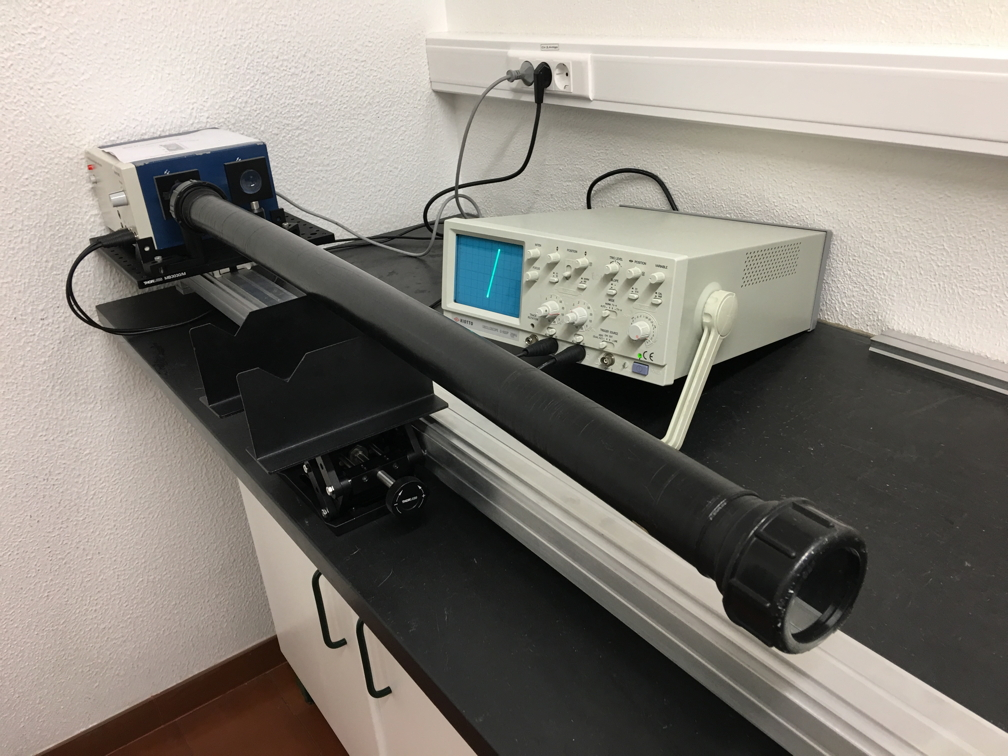
\includegraphics[width=0.6\textwidth]{fig8}
	\caption{Montagem para medição da velocidade da luz na água. \label{fig:agua}} 
\end{figure}

\subsection{\sf Medição da velocidade de propagação da luz na água}
\begin{enumerate}
\item Verifique a fase na posição inicial. Com o auxílio do banco óptico e dos dois suportes (ver figura \ref{fig:agua}), coloque cuidadosamente o tubo \emph{vazio} de modo a que o feixe incidente entre perpendicularmente à face. Pode desmontar este tubo para medir o comprimento interno do trajeto no ar/água.
\item Registe a posição dos espelhos $z_{\delta=\pi}^{\textup{tubo}}$ que produz um sinal em oposição de fase. 
\item Repita a medição para o tubo \emph{cheio de água} e obtenha o valor correspondente $z_{\delta=\pi}^{\textup{água}}$. 
\item Calcule o valor do índice de refração $n_{\textup{água}}$ obtido, a sua incerteza e o desvio à exatidão\footnote{O valor tabelado é $n_{\textup{água}}=1.3330$.}. 
\item Comente a precisão do valor da velocidade de propagação da luz obtida nos 
diferentes meios.
\end{enumerate}

\subsection{\sf Análise, conclusões e comentários finais}
Discuta a qualidade dos dados obtidos e as conclusões que pode retirar desta experiência. Comente também sobre as condições de realização da experiência, dos equipamentos utilizados e a influência de erros aleatórios e sistemáticos, identificando-os.\\
	\HRule \\[0.5cm]

%%%%%%%%%%%%%%%%%%%%%%%%%%%%%%%%%%%%%%%%%%%%%%%%%
%%%%%%%%%%%%%%%%%%%%%%%%%%%%%%%%%%%%%%%%%%%%%%%%%
%%%%%%%%%%%%%%%%%%%%%%%%%%%%%%%%%%%%%%%%%%%%%%%%%
%%%%%%%%%%%%%%%%%%%%%%%%%%%%%%%%%%%%%%%%%%%%%%%%%
%%%%%%%%%%%%%%%%%%%%%%%%%%%%%%%%%%%%%%%%%%%%%%%%%
%%%%%%%%%%%%%%%%%%%%%%%%%%%%%%%%%%%%%%%%%%%%%%%%%
%%%%%%%%%%%%%%%%%%%%%%%%%%%%%%%%%%%%%%%%%%%%%%%%%
%%%%%%%%%%%%%%%%%%%%%%%%%%%%%%%%%%%%%%%%%%%%%%%%%
%%%%%%%%%%%%%%%%%%%%%%%%%%%%%%%%%%%%%%%%%%%%%%%%%
%%%%%%%%%%%%%%%%%%%%%%%%%%%%%%%%%%%%%%%%%%%%%%%%%

\chapter{\huge{Óptica Geométrica}}
\large {\bf {Construções geométricas em lentes delgadas}}\\
	\HRule \\%[0.5cm]

\section{\sf Objectivos do trabalho}


Pretende-se estudar vários aspectos da luz do ponto de vista da óptica geométrica, tais como a reflexão e refracção entre meios, a polarização, lentes delgadas e associações de lentes. Iremos estudar a formação de imagens reais e virtuais, verificar como estas dependem das distâncias envolvidas no sistema óptico, e testar um microscópio composto.

\section{\sf Conceitos fundamentais}
\subsection{\sf Traçado de raios}
A óptica geométrica, ou óptica de raios, é uma abordagem que consiste em descrever a propagação da luz através de raios. Um raio é um modelo simplificado, na forma de uma linha, que descreve o caminho percorrido pela luz entre duas superfícies. Para descrever a propagação de um feixe de luz através de um sistema, utilizamos um conjunto de raios, que se propagam utilizando o método do \emph{traçado de raios}.
Este método é suficiente para explicar fenómenos como a reflexão e a refracção da luz e é particularmente útil na descrição de sistemas e instrumentos ópticos, sendo válida desde que as dimensões dos objectos envolvidos sejam muito maiores que o c.d.o. da luz visível ($\sim$ 0,4 a 0,7 $\mu$m).

O comportamento dos raios obedece a algumas regras simples:

\begin{enumerate}
\item Num meio uniforme, como o ar ou um vidro, um raio é uma linha recta;
\item Um meio óptico é definido por uma grandeza $n\geq1$, chamada índice de refracção;
\item Na fronteira entre dois meios, um raio é reflectido e/ou refractado, verificando-se:
\begin{itemize}
\item o ângulo de reflexão é igual ao ângulo de incidência
\item o ângulo de refracção $\theta_r$ e o ângulo de incidência $\theta_i$ (medidos relativamente à normal à superfície) obedecem à \emph{Lei de Snell-Descartes},

\begin{equation}
n_i\sin{\theta_i}=n_r\sin{\theta_r}
\end{equation}
em que $n_i$ e $n_r$ são respectivamente os índices de refracção do meio de incidência e do meio de refracção.
\end{itemize}
\end{enumerate}
%%%%%%%%%%%%
\begin{figure}
\begin{center}
	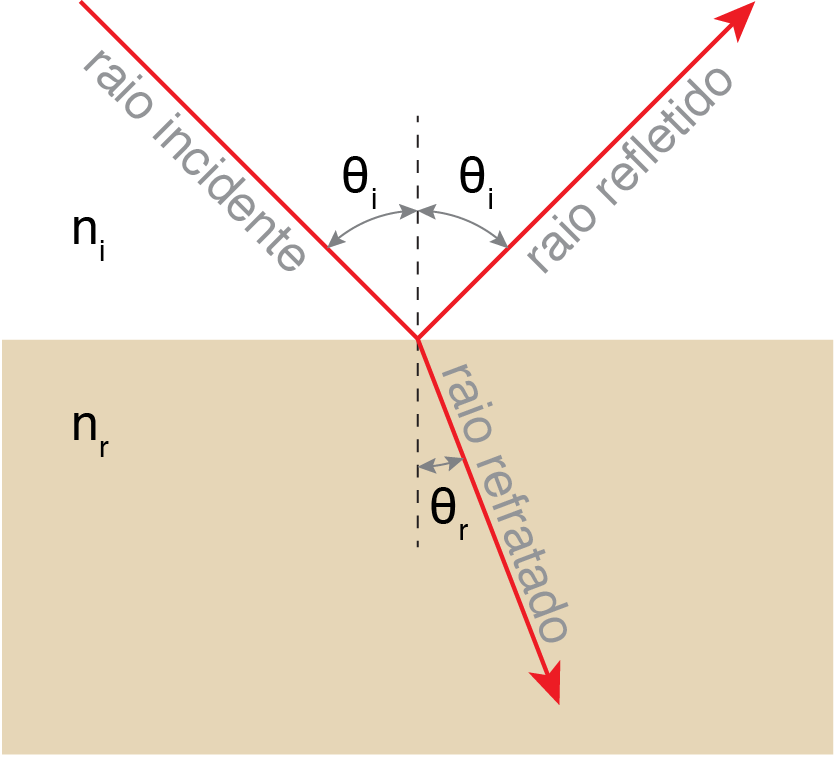
\includegraphics[width=0.4\textwidth]{1-snell}
	\caption{Raio reflectido e refractado na fronteira entre dois meios.}
	 \label{fig:snell}
\end{center}
\end{figure}
%%%%%%%%%%%%

\subsection{\sf Reflexão, refracção e polarização}

A eficiência com que um feixe luminoso é reflectido ou refractado numa fronteira entre dois meios de índices de refracção $n_1$ e $n_2$ depende, entre outros, do ângulo de incidência e da polarização da luz. A Fig. \ref{fig:brewster} mostra como varia a reflectividade de uma superfície de vidro em função do ângulo de incidência, para polarizações horizontal e vertical (admitindo que o plano de incidência e reflexão é horizontal). Para um ângulo específico, designado \emph{ângulo de Brewster} e dado por $\theta_B=\arctan(n_2/n_1)$, a componente horizontal da polarização não é reflectida, pelo que a luz reflectida fica com polarização vertical. Esta é uma forma de criar luz polarizada a partir de uma fonte não-polarizada. A figura ilustra também a geometria dos raios luminosos numa separação entre dois meios, no caso de incidência em ângulo de Brewster. Como se pode apreciar, nessa configuração o raio reflectido e o raio refractado fazem entre si um ângulo de 90$^\circ$.

Pode-se polarizar a luz emitida por uma fonte não-polarizada através de um simples filtro polarizador (ou \textit{polaroide}). Orientando o ângulo do filtro relativamente à direcção dos raios luminosos, é possível definir a direcção de polarização (Fig. \ref{fig:pol-luz}).

%%%%%%%%%%%%
\begin{figure}[h]
\begin{center}
	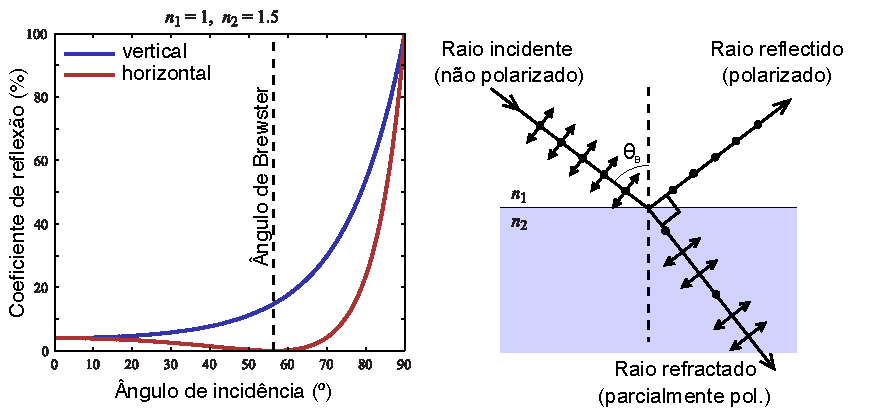
\includegraphics[width=0.85\textwidth]{2-brewster}
	\caption{Reflectividade vs. ângulo de incidência e direcção de polarização (esq.) e geometria para ângulo de Brewster (dir.). \label{fig:brewster}} 
\end{center}
\end{figure}
%%%%%%%%%%%%

\begin{figure}[t]
\centering 
	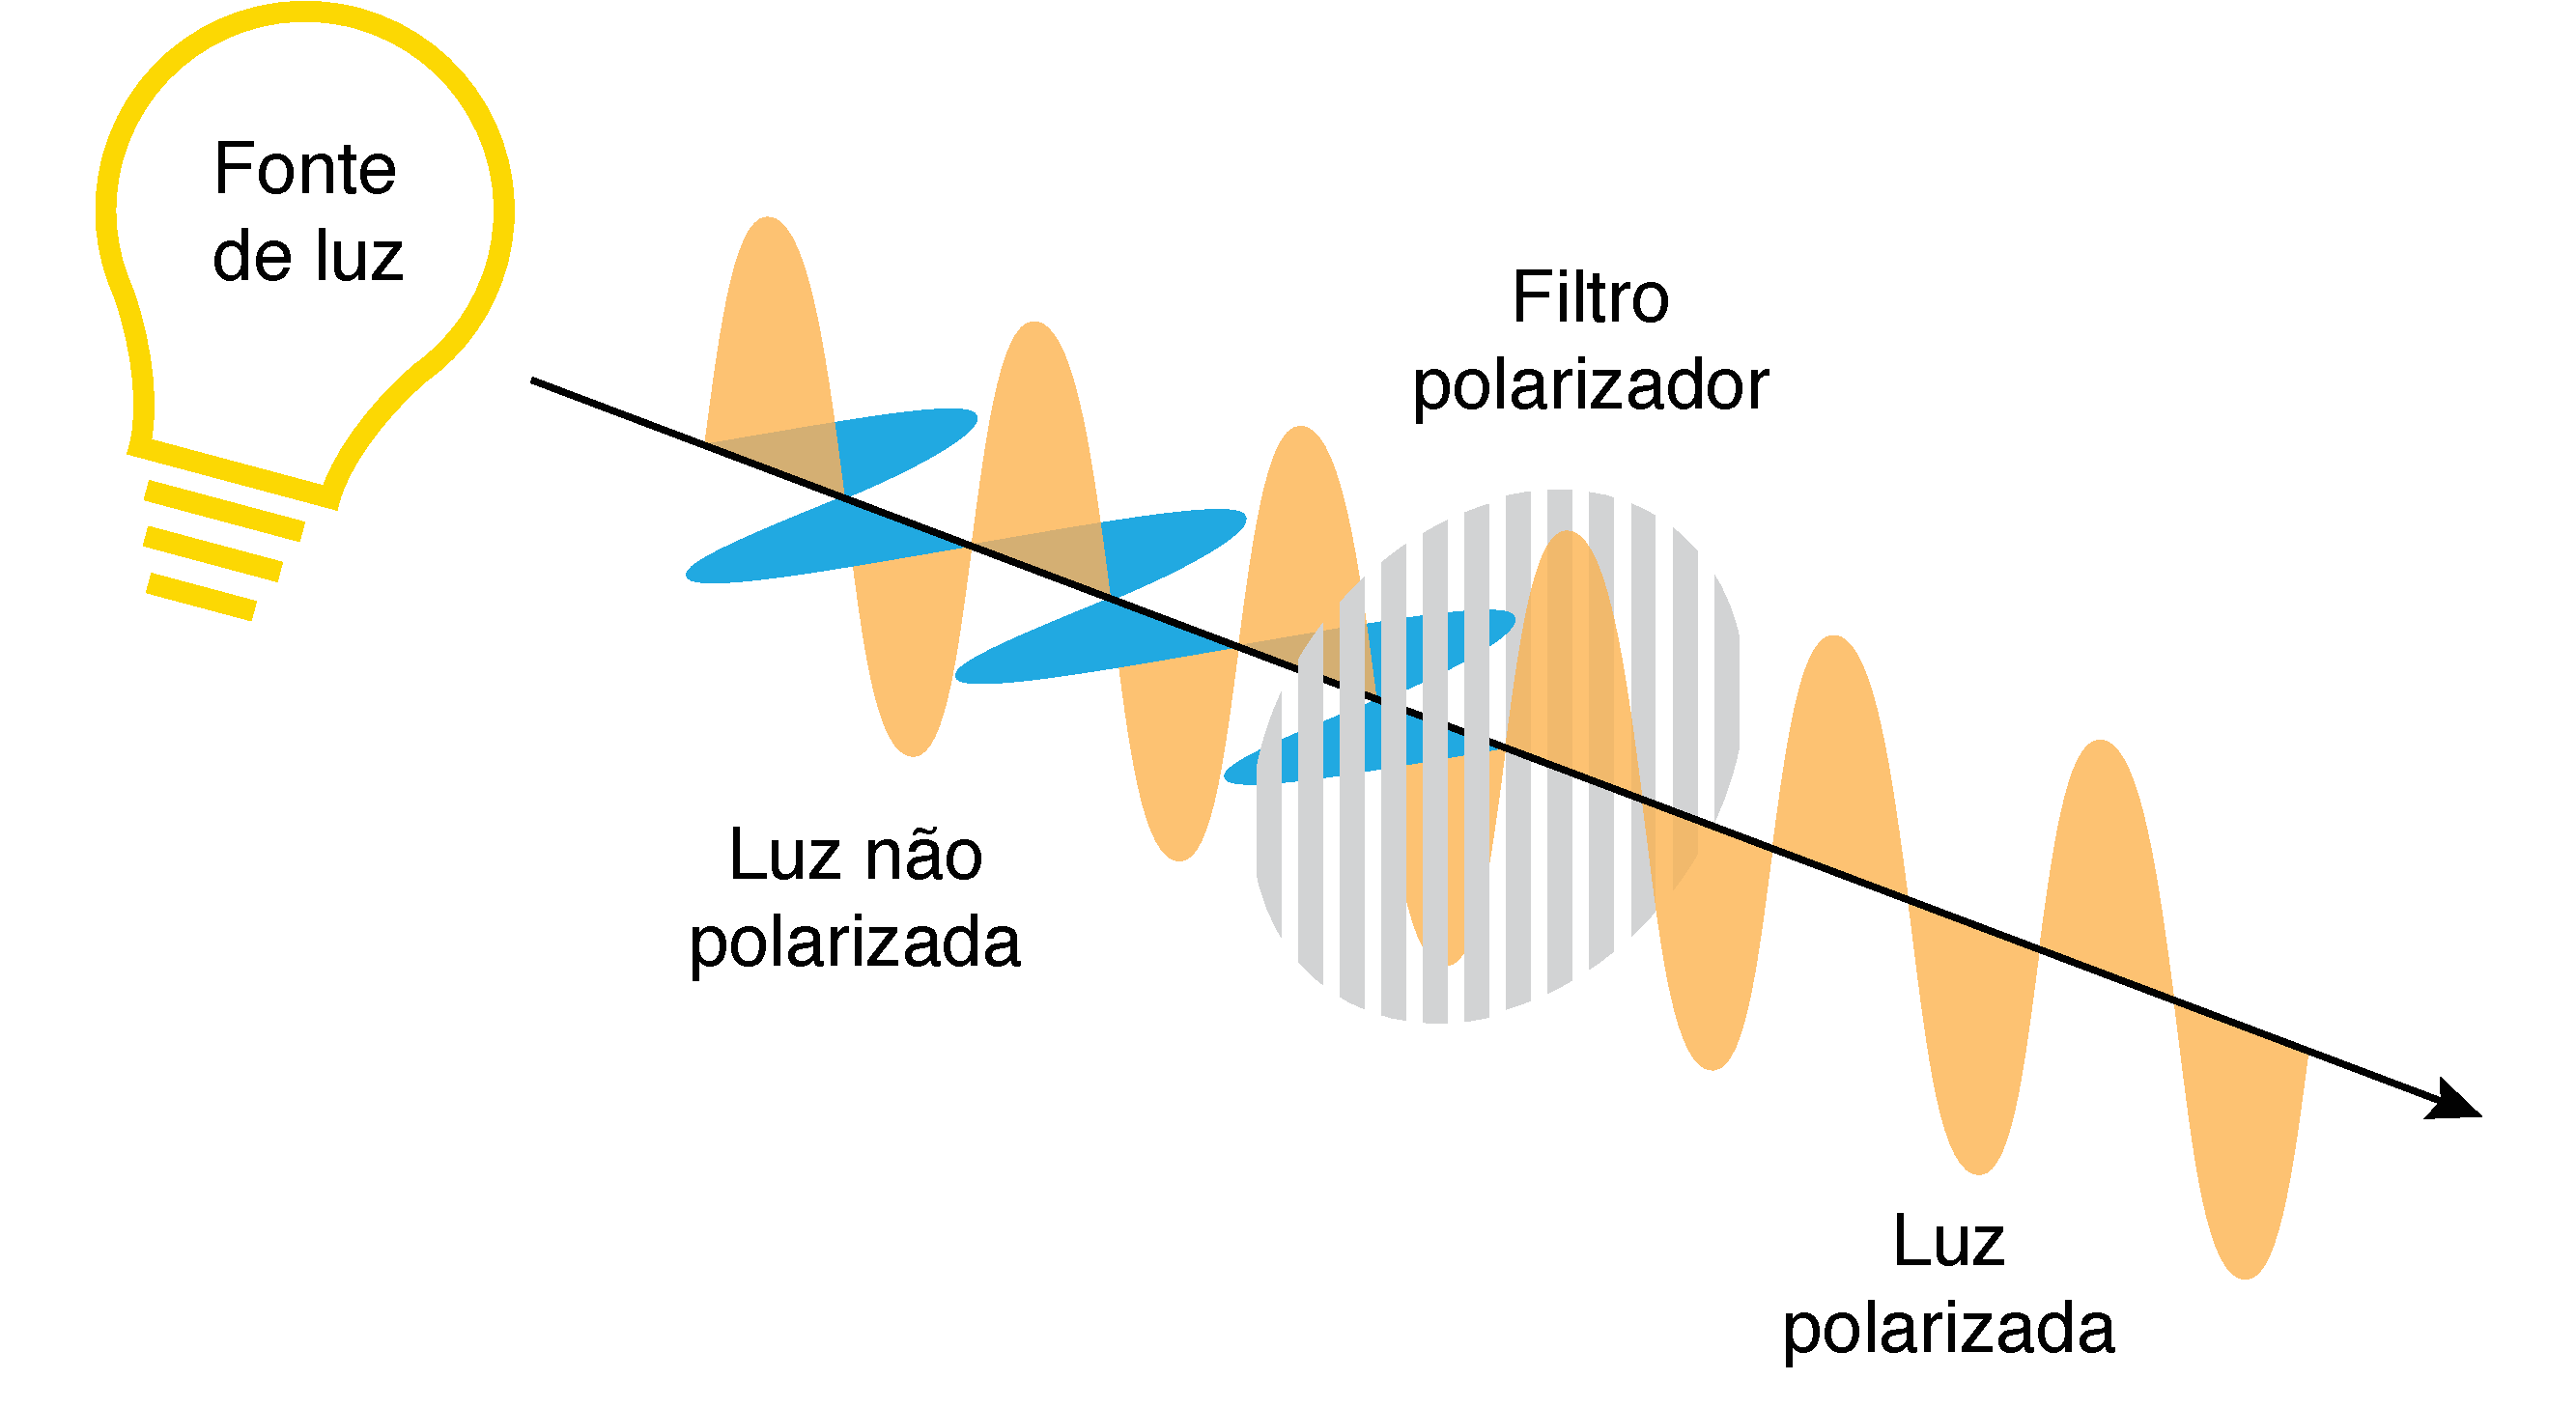
\includegraphics[width=0.8\textwidth]{2-pol-luz}
	\caption{Obtenção de luz polarizada (verticalmente, no caso da figura) através de um filtro polarizador. \label{fig:pol-luz}} 
\end{figure}






%%%%%%%%%%%%%%%%%%%%%%%%%%%%%%%%%%%%%%%%%%%%%%%%%%
%%%%%%%%%%%%%%%%%%%%%%%%%%%%%%%%%%%%%%%%%%%%%%%%%%
\section{\sf Construções geométricas em lentes delgadas}

Uma das principais aplicações da óptica geométrica consiste no estudo da formação de imagens: dado um \emph{objecto} numa dada posição, como desenhar um sistema óptico que permita transferir uma \emph{imagem} desse objecto para uma posição diferente? É um problema que tem aplicações desde o olho humano até ao desenho de lentes e fibras ópticas.

 Um \emph{objecto} iluminado uniformemente é considerado como uma fonte de raios, emitidos em todas as direcções. Podemos escolher um ponto no objecto e um conjunto adequado de raios, e traçar o seu percurso através do sistema até encontrar o correspondente ponto na \emph{imagem}. Por convenção, desenha-se o sistema óptico em torno de um eixo, que coincide com o seu eixo geométrico, e os raios propagam-se da esquerda para a direita. 



\subsection{\sf Aproximações}
Utilizaremos as duas seguintes aproximações comuns, que facilitam grandemente os cálculos a efectuar (Fig. \ref{fig:fig2}):

\emph{Lentes delgadas} -- uma lente é considerada \emph{delgada} quando a sua espessura $d$ é desprezável face à sua distância focal $f$.

\emph{Aproximação paraxial} -- admitimos que todos os raios envolvidos são \emph{paraxiais}, isto é, (\emph{i}) situam-se próximo do eixo óptico e (\emph{ii}) o ângulo $\alpha$ que fazem com esse eixo permite utilizar as aproximações $\sin \alpha \approx \alpha$ e  $\tan \alpha \approx \alpha\,$, tipicamente válidas para $\alpha \lesssim 5^{\circ}$.

\begin{figure}
	[!ht]  \centering 
	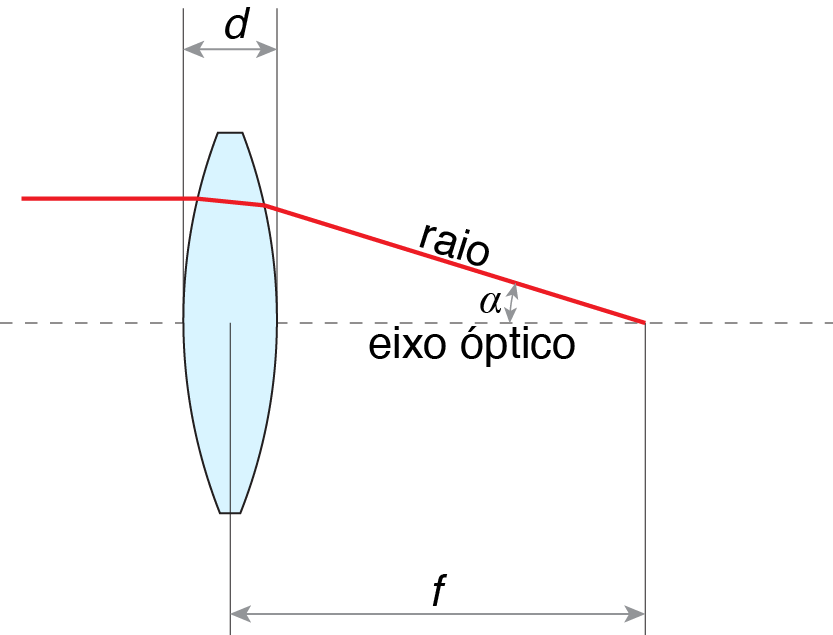
\includegraphics[width=0.4\textwidth]{2-definicoes}
 	\caption{\label{fig:fig2} Definições utilizadas: $f$ -- distância focal, $d\ll f$ -- espessura da lente delgada, $\alpha$ -- ângulo entre o raio e o eixo óptico.} 
\end{figure}



%%%%%%%%%%%%%%%%%%%%%%%%%%%%%%%%%%%%%%%%%%%%%%%%%%
\subsection{\sf Convenções}
A Fig. \ref{fig:convencoes} ilustra os principais parâmetros do traçado de raios através de uma lente simples.

\begin{itemize}
\item O objecto $AB$ fica (por definição) do lado esquerdo da lente, a uma distância $d_O>0$ desta; caso o objecto esteja do lado direito, temos $d_O<0$ (que é o caso do "objecto virtual" abordado mais à frente)
\item A imagem $A'B'$ está do lado direito da lente, a uma distância $d_I>0$ desta; caso a imagem esteja do lado esquerdo, temos $d_I<0$
\item $F_0$ é a distância focal do lado do objecto, $F_I$ é a distância focal do lado da imagem. No caso de uma lente fina, ambas são iguais a $f$, e marcam-se para auxiliar no traçado.
\end{itemize}

\begin{figure}
	[!b]  \centering 
	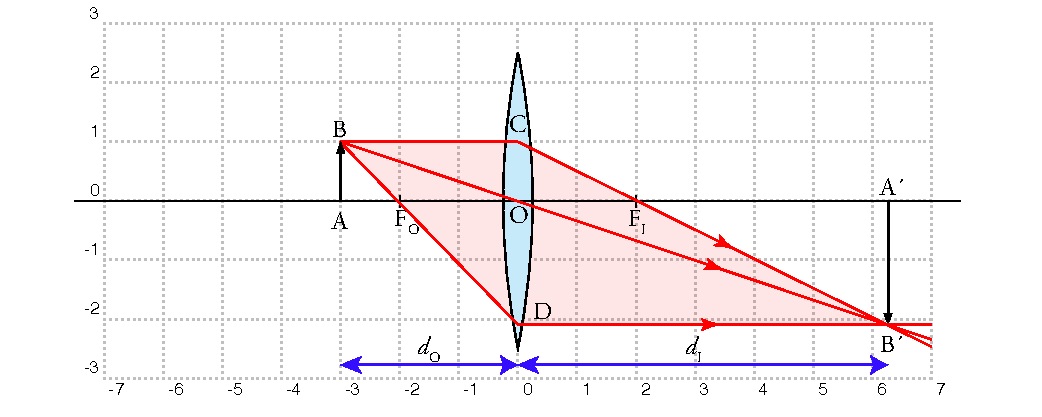
\includegraphics[width=0.9\textwidth]{3-convencoes}
	\caption{Convenções utilizadas para formação de imagens por lentes. \label{fig:convencoes}} 
\end{figure}

O raios ópticos que emergem de um dado objecto atravessam a lente e dão origem a uma imagem. As imagens dizem-se \emph{reais} quando os raios de luz passam de facto na posição da imagem, isto é, raios que saem do plano do objecto convergem no plano da imagem; e dizem-se \emph{virtuais} quando os raios não passam na imagem, mas esta é visível através da lente. As imagens reais podem ser projectadas num alvo, as virtuais não. Um bom exemplo é considerar a imagem de uma lâmpada brilhante: ao passar a mão pelo plano da imagem, se estar for real sente-se o calor, mas se for virtual parecerá apenas "flutuar" no espaço.

De seguida, vamos analisar a formação de imagens para lentes convergentes ($f>0$) e divergentes ($f<0$) em função da posição relativa do objecto e do foco da lente, e derivar relações úteis para lentes delgadas.



%%%%%%%%%%%%%%%%%%%%%%%%%%%%%%%%%%%%%%%%%%%%%%%%%%
\subsection{\sf Objecto e imagem - focos conjugados e ampliação transversal}
Considere de novo a Fig. \ref{fig:convencoes}. Cada ponto do objecto em $d_O$ tem um único ponto correspondente na imagem em $d_I$. Isto implica que, caso colocássemos o objecto em $d_I$, a imagem seria formada em $d_O$. Chama-se a estas posições \emph{focos conjugados}.
Pela semelhança de triângulos temos as seguintes relações entre as dimensões do objecto e da imagem:

\begin{IEEEeqnarray}{rClrCl}
%\begin{array}{ccccc}
\Delta ABF_O \sim \Delta ODF_O  &\to & AB/A'B' = AF_O / F_O 0 &\to & AB/A'B' =  \frac{d_O-f}{ f} \label{eq:1} \\
\Delta ABO\sim \Delta A'B'O    &\to & AB/A'B' = AO / O A' &\to & AB/A'B' = d_O / d_I \label{eq:2} \\
\Delta COF_I \sim \Delta A'B'F_I  &\to & AB/A'B' = OF_I / F_I A' &\to & AB/A'B' =  \frac{f}{ d_I-f} \label{eq:3} 
\end{IEEEeqnarray}

Das expressões (\ref{eq:1}) e (\ref{eq:3}) obtemos a equação dos focos conjugados:
 
 \begin{equation}
	\label{eq:focosconjug}
    \fbox{
        $ \displaystyle
	\frac{1}{f} = \frac{1}{d_O} +\frac{1}{d_I} 
        $
    }
% \qquad \text{ equação dos focos conjugados}
\end{equation}

Uma forma alternativa e muitas vezes conveniente de exprimir esta relação consiste em utilizar as distâncias do objecto e da imagem aos respectivos focos. Designando estas distâncias por $x_O=AF_O$ e $x_I=A'F_I$, tem-se $d_O=f+x_O$ e $d_I=f+x_I$. Substituindo na expressão acima, obtém-se a chamada formulação de Newton para a equação dos focos conjugados:

 \begin{equation}
	\label{eq:focosconjugnewton}
    \fbox{
        $ \displaystyle
	x_Ox_I = f^2
        $
    }
% \qquad \text{ equação dos focos conjugados}
\end{equation}

Por outro lado, sendo $AB$ e $A'B'$ respectivamente as dimensões lineares transversais do objecto e da imagem, usamos a igualdade (\ref{eq:2}) para definir a \emph{ampliação transversal} $A$ como:

 \begin{equation}
    \fbox{
        $ \displaystyle
A =  \frac{A'B'}{ AB} =\frac{d_I}{d_O}
$
}
\end{equation}
 
A imagem é \emph{direita} se $A<0$ e \emph{invertida} se $A>0$. Podemos usar estas duas equações para, dados $f$ e $d_O$, determinar as seguintes expressões para a posição da imagem $d_I$ e a respectiva ampliação $A$:
 
\begin{eqnarray}
A&=&\frac{1}{\frac{d_O}{f}-1}\\
d_I&=&d_OA
\end{eqnarray}

 
Como exemplo, temos no caso da Fig. \ref{fig:convencoes}: $d_O>f \to A> 0\,; d_I > 0$. A imagem resultante é \emph{real} e \emph{invertida}.

%%%%%%%%%%%%%%%%%%%%%%%%%%%%%%%%%%%%%%%%%%%%%%%%%%
\subsubsection{\sf Lente convergente ($f>0$) -- Imagem real}
Este caso verifica-se para $d_O>f$, a imagem é real é pode ser projectada. A imagem é menor ($A<1$) que o objecto se $d_O>2f$ ou maior ($A>1$) se $2f>d_O>0$. Um exemplo do primeiro caso é uma máquina fotográfica: a imagem é posicionada no sensor da câmara, e é (tipicamente) menor que o objecto fotografado. Verifica-se  \fbox{$0 < A \le 1$ } pois

\begin{equation}
\infty > d_O \ge 2 f \quad \to \quad f < d_I \le 2 f  \quad \to \quad 0<A\le 1
\end{equation}

Um exemplo do segundo caso é um projetor de cinema ou de imagem de computador: a imagem é posicionada num écran, e é maior que o objecto (película ou chip). Verifica-se  \fbox{$1 \le A < \infty$} pois

\begin{equation}
f < d_O \le 2 f  \quad \to  \quad  \infty > d_I \ge 2f \quad \to \quad \infty>A\ge 1
\end{equation}

%%%%%%%%%%%%%%%%%%%%%%%%%%%%%%%%%%%%%%%%%%%%%%%%%%
\subsubsection{\sf Lente convergente ($f>0$) -- Imagem virtual}

Este caso verifica-se quando $d_O<f$, por exemplo quando utilizamos uma lupa para ver objectos com um tamanho aumentado, e está esquematizada na Fig. \ref{fig:fig4}. Dependendo da posição $d_O$, verificam-se as seguintes relações

%\begin{figure}
%	[!htb]  \centering 
%	\includegraphics[width=0.8 \textwidth]{lupa}
%	\caption{. \label{fig:lupa}} 
%\end{figure}

\begin{IEEEeqnarray}{rCl}
0 < d_O \le \frac{f}{2} \qquad & 0 > d_I \ge -f \quad& -1 >A \ge -2\\
\frac{f}{2} \le d_O < f \qquad& -f\ge d_I >-\infty \quad& -2 > A > -\infty
\end{IEEEeqnarray}

Repare-se que resulta $d_I<0$ (a imagem está do mesmo lado que o objecto) e $A<0$ pelo que a imagem é (\emph{i}) virtual e (\emph{ii}) direita, para um observador colocado à direita da lente.

\begin{figure}
\begin{center}
\psscalebox{0.75}{
\begin{pspicture}[showgrid=true](-7,-3)(7,3)
\rput(0,0){\lens[lensType=CVG,focus=4.5,OA=-2.7,AB=1,XO=0,YO=0,nameF=F_O,nameFi=F_I,spotAi=0,drawing=true,rayColor=white]}
\psline[linecolor=red,linestyle=dashed](B')(F')
\psline[linecolor=red,linestyle=dashed](B')(B)
\psline[linecolor=red](B)(0,1)
\psline[linecolor=red](B)(2.7,-1)
\psline[linecolor=red](0,1)(F')
\psset{linecolor=red}
\Arrows[posStart=0,length=1](B)(0,1)
\Arrows[posStart=2,length=3](B)(0,0)
\Arrows[posStart=0,length=3](0,1)(F')
\rput(8,0){\psset{linecolor=black}\eye}
\end{pspicture}
}
\caption{Formação de imagem virtual com uma lente convergente. \label{fig:fig4}} 
\end{center}
\end{figure}

%%%%%%%%%%%%%%%%%%%%%%%%%%%%%%%%%%%%%%%%%%%%%%%%%%



\begin{figure}[b]
 \centering 
	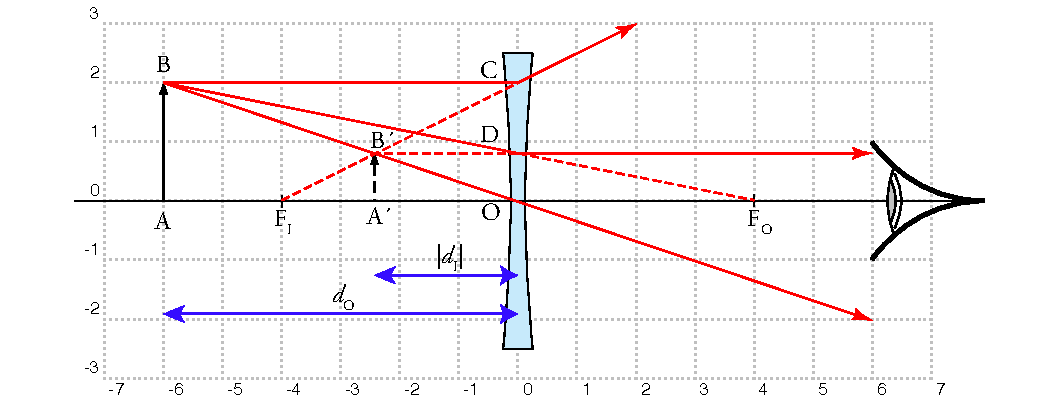
\includegraphics[width=0.7\textwidth]{5-DivVirt}
	\caption{Formação de imagem virtual com uma lente divergente. \label{fig:DivVirt}} 
\end{figure}

\subsubsection{\sf Lente divergente ($f<0$)}
Considere-se a situação representada na Fig. \ref{fig:DivVirt}, que mostra uma lente divergente ($f<0$) e um objecto  $AB$ ($d_O>0$). Note-se que, no caso da lente divergente, os pontos $F_O$ e $F_I$ trocam de posição. Nesta configuração a imagem resultante $A'B'$ é sempre \emph{virtual}  e \emph{direita} com $d_I <0$ (imagem do mesmo lado do objeto), pois

\begin{equation*}
f<0; \quad d_O> 0 \quad \to  \quad A<0;  \quad  d_I <0  
\end{equation*}

Podemos verificar que a equação (\ref{eq:focosconjug}) se mantém válida neste caso, recorrendo à semelhança de triângulos:
\begin{IEEEeqnarray}{rClrCl}
%\begin{array}{ccccc}
\Delta ABO \sim  \Delta A'B'O  & \to & AB/A'B' = \frac{d_0}{d_I} & \to & -\infty < A < 0 \label{eq:diver1} \\
\Delta ABF_0\sim \Delta ODF_O   &\to & \frac{d_0 + |f|}{|f|} = AB/A'B' & \to & \frac{d_0 + |f|}{|f|} = \frac{d_0 }{d_I}  \label{eq:diver2} \\
\Delta F_I OC \sim \Delta F_I A'B'  &\to & \frac{|f|}{|f| - |d_I|} =AB/A'B'  &  \to &  \frac{|f|}{|f| - |d_I|} = \frac{d_0 }{|d_I|} 
\end{IEEEeqnarray}

Nestas expressões, que descrevem distâncias, foi necessário  utilizar os valores em módulo de $f$ e de $d_I$, que são ambos negativos. Fazendo agora as substituições $|f|\to -f$ e $|d_I|\to -d_I$ recupera-se a equação dos focos conjugados.


%%%%%%%%%%%%%%%%%%%%%%%%%%%%%%%%%%%%%%%%%%%%%%%%%%
\subsection{\sf Objectos virtuais}

Em determinadas situações, podemos lidar com "objectos virtuais"  ($d_O<0$), isto é, os raios ópticos têm origem não num objecto sólido, mas num plano do espaço, e estamos interessados em estudar a sua propagação a partir desse plano e a formação da imagem correspondente. Um exemplo típico consiste em estudar a formação da imagem de uma imagem primária. Nestes casos, o objecto virtual é identificado a tracejado no diagrama de raios, como ilustrado nos exemplos em baixo.

%%%%%%%%%%%%%%%%%%%%%%%%%%%%%%%%%%%%%%%%%%%%%%%%%%
\subsubsection{\sf Lente convergente $f>0$}
A Fig. \ref{fig:ConvVirt} representa um objecto virtual ($d_O<0$, à direita da lente) e a correspondente imagem. A imagem resultante é real ($d_I>0$, também à direita) e direita ($A<0$), verificando-se

\begin{IEEEeqnarray}{rCl}
 d_O < 0 ; \quad &&  f > 0 \quad \to \quad A<0  \nonumber\\
\frac{d_I}{-|d_O|}  & =&  \frac{f}{-|d_O| -f}     \nonumber
\end{IEEEeqnarray}



\begin{figure}[t]
 \centering 
	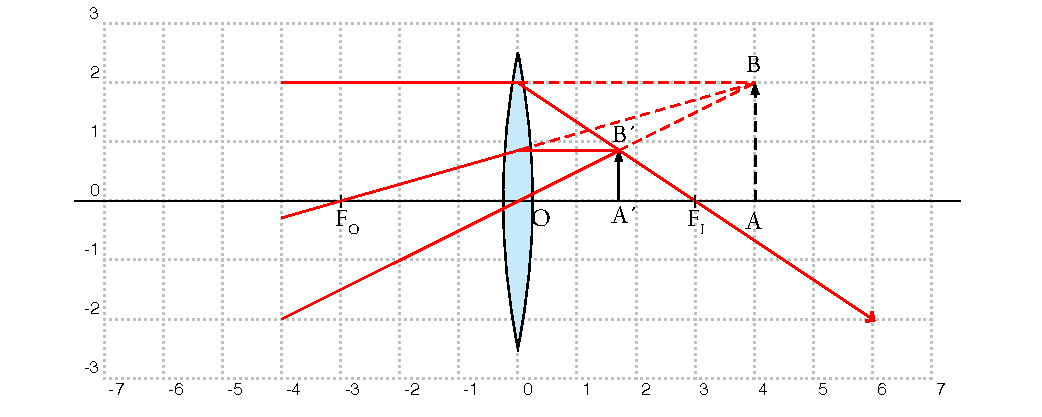
\includegraphics[width=0.7\textwidth]{6-ConvVirt}
	\caption{Lente convergente com objecto virtual e imagem real. \label{fig:ConvVirt}} 
\end{figure}

%%%%%%%%%%%%%%%%%%%%%%%%%%%%%%%%%%%%%%%%%%%%%%%%%%



\begin{figure}[b]
	\centering 
	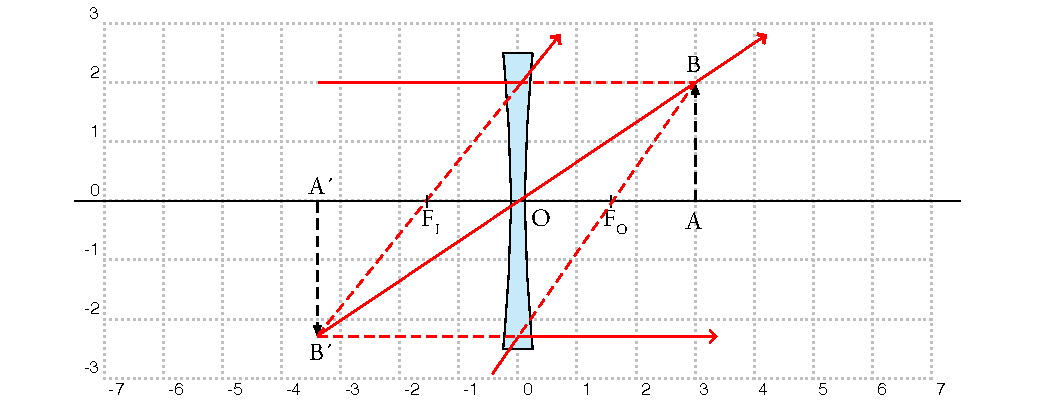
\includegraphics[width=0.7\textwidth]{7-DivVirtVirt}
	\caption{Lente divergente com objecto virtual e imagem virtual. \label{fig:DivVirtVirt}} 
\end{figure}

\subsubsection{\sf Lente divergente $f<0$ -- Imagem virtual}
A Fig. \ref{fig:DivVirtVirt} representa um objecto virtual ($d_O<0$, à direita da lente) para uma lente divergente ($f<0$) e a correspondente imagem. Na situação da figura, o objecto está à direita do foco $F_O$: $|d_O|>|f|$. Verifica-se assim:

\begin{IEEEeqnarray}{rCl}
 d_O < 0 & &  f < 0   \nonumber\\
\frac{d_I}{|d_O|}  & =&  \frac{|f|}{|d_O| -|f|}     \nonumber
\end{IEEEeqnarray}

A imagem resultante é também virtual $d_I<0$, à esquerda da lente) e invertida ($A>0$), verificando-se as seguintes relações em função da distância:
\begin{equation}
|d_O|  =  \left\{
\begin{array}{rl}
|d_O|   = |f|:  &   |d_I| \to \infty, \quad A \to \infty ,\\
|f| < |d_O|   < 2|f|:  &   |d_I|  > |d_O| , \quad A  >1  ,\\
|d_O|   = 2|f|:  &   |d_I| = |d_O|, \quad A =1  ,\\
|d_O|  > 2|f|:   & |d_I|  <|d_O| , \quad 0 < A  <1  .
\end{array}  \right.
%f<0 \quad \to   d_O> 0 ; \quad  d_I <0  
\end{equation}

%%%%%%%%%%%%%%%%%%%%%%%%%%%%%%%%%%%%%%%%%%%%%%%%%%
\subsubsection{\sf Lente divergente $f>0$ - Imagem real}

A Fig. \ref{fig:DivVirtReal} representa um objecto virtual ($d_O<0$, à direita da lente) para uma lente divergente ($f<0$) e a correspondente imagem. Na situação da figura, o objecto está à esquerda do foco $F_O$: $|d_O|<|f|$. Verifica-se assim:

\begin{figure}
	[!htb]  \centering 
	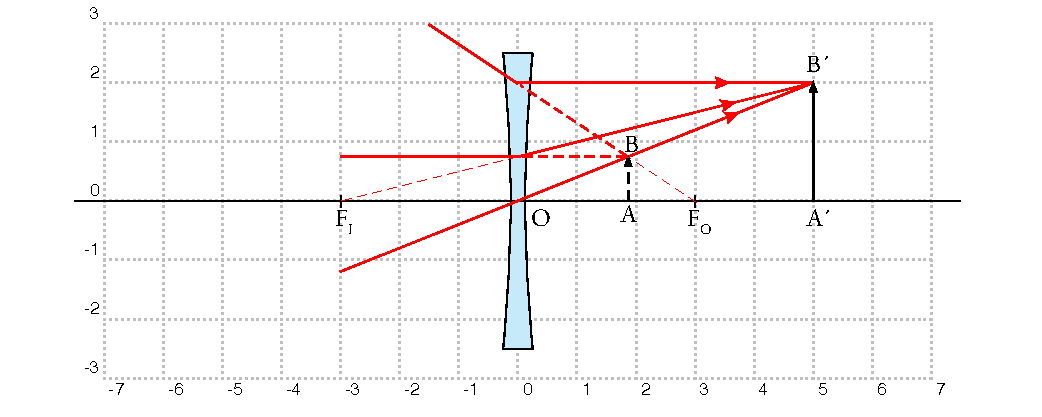
\includegraphics[width=0.7\textwidth]{8-DivVirtReal}
	\caption{Lente divergente com objecto virtual e imagem real. \label{fig:DivVirtReal}} 
\end{figure}

\begin{IEEEeqnarray}{rCl}
 d_O < 0 & &  f < 0   \nonumber\\
\frac{d_I}{|d_O|}  & =&  \frac{|f|}{|f|-|d_O|} \quad \to \quad A=\frac{d_I}{d_O} =\frac{f}{d_O-f}<0     \nonumber
\end{IEEEeqnarray}



A imagem resultante é agora real ($d_I>0$, à direita da lente) e direita ($A<0$), verificando-se as seguintes relações em função da distância:
\begin{equation}
|d_O|  =  \left\{
\begin{array}{rl}
|d_O|   \to |f|:  &   |d_I| \to \infty, \quad A \to -\infty ,\\
|d_O|   = |f|/2:  &   |d_I| = f, \quad A =-2  ,\\
|d_O|  =0:  & |d_I|  =0 , \quad A=-1.
\end{array}  \right.
%f<0 \quad \to   d_O> 0 ; \quad  d_I <0  
\end{equation}



%%%%%%%%%%%%%%%%%%%%%%%%%%%%%%%%%%%%%%%%%%%%%%%%%%
%%%%%%%%%%%%%%%%%%%%%%%%%%%%%%%%%%%%%%%%%%%%%%%%%%

\section{\sf Associação de lentes delgadas}

Para duas lentes delgadas de distâncias focais $f_1$ e $f_2$ afastadas de $D$ (para $D \ll f_1,f_2$) pode calcular-se a distância focal equivalente do conjunto através de: 

 \begin{equation}
	\label{eq:assoclentes}
    \fbox{
        $ \displaystyle
	\frac{1}{f_{equiv}} = \frac{1}{f_1} + \frac{1}{f_2} - \frac{D}{f_1 \,f_2} 
        $
    }
\end{equation}

A dificuldade
%quando se usa o método direto quer dos focos conjugados, para 
na determinação da distância focal equivalente ${f_{equiv}}$ é a medição das distâncias $d_O$ e $d_I$ 
(que são diferentes das distância do objecto e da imagem às superfícies das lentes ou aos seus planos médios).

Uma abordagem preferível consiste em usar a equação (\ref{eq:focosconjug}) separadamente para cada uma das lentes, e considerar que a \emph{primeira imagem} (real ou virtual) irá constituir-se como o \emph{objecto} para a segunda lente. Neste caso, as regras descritas acima para o traçado de raios de lentes individuais aplicam-se consecutivamente:
\begin{enumerate}
\item  A partir da posição do objecto $AB$ e do tipo da primeira lente $L_1$, determina-se a posição da imagem intermédia $A'B'$
\item  A partir da posição da imagem intermédia (agora tomada como objecto da segunda lente) e do tipo da segunda lente $L_2$, determina-se a posição da imagem final $A''B''$
\end{enumerate}
Vamos aplicar este método para várias combinações de lentes convergentes e divergentes.

%%%%%%%%%%%%%%%%%%%%%%%%%%%%%%%%%%%%%%%%%%%%%%%%%%
\subsection{\sf Lente convergente - lente convergente}
A Fig. \ref{fig:DuplaConvConv1} representa duas lentes convergentes, $L_1$ e $L_2$, de distâncias focais $f_1$ e $f_2$ respectivamente, separadas de uma distância $D$. O objecto (real) $AB$ situa-se à esquerda de $L_1$, e tem uma imagem $A'B'$ por intermédio de $L_1$. Esta imagem constitui-se como objecto virtual para $L_2$, resultando no final a imagem $A''B''$. Esta é a montagem mais simples de um \textbf{telescópio}, a partir do qual se podem obter grandes ampliações.

\begin{figure}	[t]  \centering 
	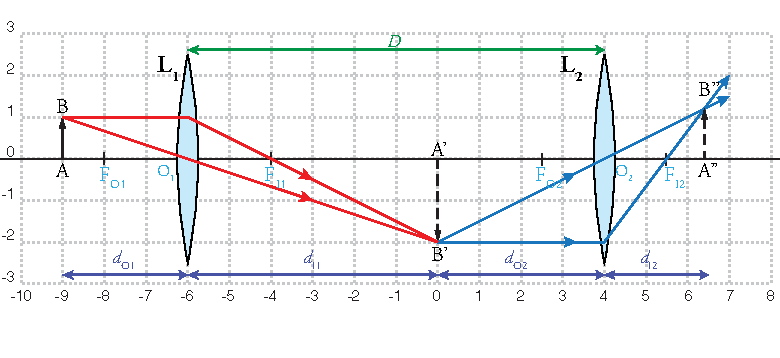
\includegraphics[width=0.9\textwidth]{9-DuplaConvConv1}
	\caption{Sistema de duas lentes convergentes, com objecto intermédio real. \label{fig:DuplaConvConv1}} 
\end{figure}

Apliquemos as equações de lentes individuais para cada caso:

\begin{equation}
|d_O|  =  \left\{
\begin{array}{llll}
 \frac{1}{d_{O_1}} +  \frac{1}{d_{I_1}}   = \frac{1}{f_1}  & d_{O_1} = AO_1 & d_{I_1} = O_1A' & f_1 = O_1 F_{O_1} = O_1\,F_{I_1} \\
 \frac{1}{d_{O_2}} +  \frac{1}{d_{I_2}}   = \frac{1}{f_2}  & d_{O_2} = A'O_2 & d_{I_2} = O_2\,A'' & f_2 =  F_{O_2}\,O_2\, = O_2\,F_{I_2} \\
O_1\,O_2 = D = d_{I_1} + d_{O_2}
\end{array}  \right.
\label{eq:assoclentes_2}
\end{equation}

\begin{figure}	[b]  \centering 
	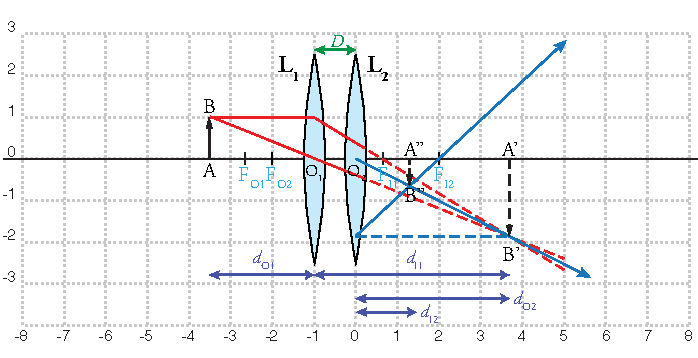
\includegraphics[width=0.9\textwidth]{10-DuplaConvConv2}
	\caption{Duas lentes convergentes, com objecto intermédio virtual. \label{fig:DuplaConvConv2}} 
\end{figure}

Estas três expressões permitem calcular o valor de uma das incógnitas, conhecidos os valores das outras. Por exemplo, uma aplicação comum desta montagem consiste em determinar o valor de uma distância focal desconhecida $f_2$, conhecidos os valores de $f_1$, $d_{O_1}$, $d_{I_2}$ e $D$.

As mesmas expressões aplicam-se para o caso de uma imagem obtida por uma lente $L_1$ que passa a ser um “objecto” virtual para $L_2$, isto é, em que $d_{O2}<0$, situação ilustrada na Fig. \ref{fig:DuplaConvConv2}.



%%%%%%%%%%%%%%%%%%%%%%%%%%%%%%%%%%%%%%%%%%%%%%%%%%
\subsection{\sf Lente convergente - lente divergente}
O outro sistema de lente dupla de interesse é o caso em que temos uma lente convergente e uma divergente separadas de $D$, ilustrado na Fig. \ref{fig:DuplaConvDiv1}, em que $L_1$ é convergente e $L_2$ é divergente. A lente $L_1$ produz uma imagem intermédia $A'B'$ real e invertida, que é o objecto (real) de $L_2$. Uma vez que a segunda lente é divergente, a sua imagem $A''B''$ (a imagem final) é sempre virtual e invertida.

\begin{figure}	[t]  \centering 
	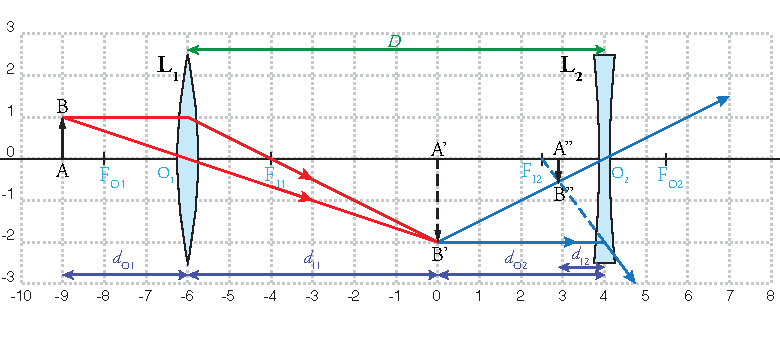
\includegraphics[width=0.9\textwidth]{11-DuplaConvDiv1}
	\caption{Sistema de lente convergente e divergente  com objecto intermédio real: a imagem final é virtual e invertida. \label{fig:DuplaConvDiv1}} 
\end{figure}

A Fig. \ref{fig:DuplaConvDiv2} ilustra a situação em que $A'B'$ está numa posição à direita de $L_2$: é uma imagem real (de $L_1$) mas um objecto virtual (de $L_2$), já que $d_{O2}<0$. A imagem $A''B''$ resultante é real e invertida.

\begin{figure}	[b] 
\begin{center}
	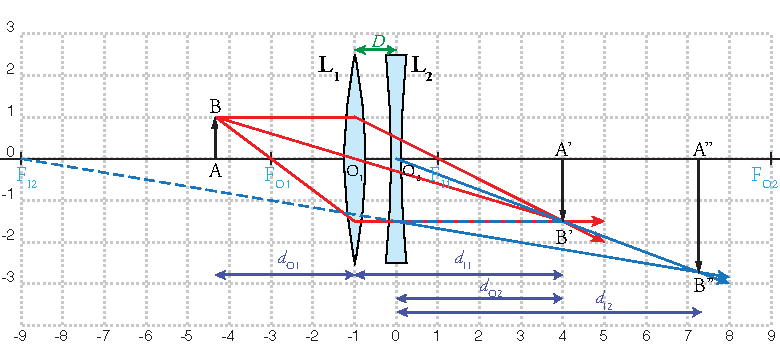
\includegraphics[width=0.9\textwidth]{12-DuplaConvDiv2}
	\caption{Sistema de lente convergente e divergente com objecto intermédio virtual: a imagem final é real e invertida. \label{fig:DuplaConvDiv2}} 
\end{center}
\end{figure}

\begin{figure}	[!htb]  
\begin{center}
	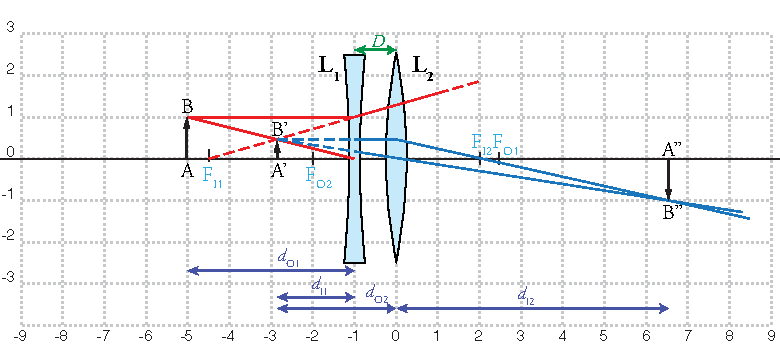
\includegraphics[width=0.9\textwidth]{13-DuplaConvDiv3}
\end{center}
	\caption{Sistema de lente convergente e divergente.  \label{fig:DuplaConvDiv3}} 
\end{figure}


Por fim, se nesta montagem permutarmos $L_1$ e $L_2$ (Fig. \ref{fig:DuplaConvDiv3}), obtém-se também uma imagem real  $A''\,B''$, desde que a distância $d_{O1}=A\,O_1$ seja idêntica.
Em qualquer destas situações, pode sempre calcular-se $f_2 < 0$ usando o conjunto das três equações (\ref{eq:assoclentes_2}).
\clearpage

%%%%%%%%%%%%%%%%%%%%%%%%%%%%%%%%%%%%%%%%%
%%%%%%%%%%%%%%%%%%%%%%%%%%%%%%%%%%%%%%%%%
%%%%%%%%%%%%%%%%%%%%%%%%%%%%%%%%%%%%%%%%%


\section{\sf Instrumentos ópticos}
Um instrumento óptico é um dispositivo baseado nos princípios da óptica cujo objectivo é auxiliar a visão humana. Nestes sistemas, designamos por \emph{objectiva} a lente que está do lado do objeto AB e por \emph{ocular} aquela que está do lado do observador, com distâncias focais $f_{obj}$ e $f_{ocu}$ respetivamente. Em ambos os casos, a ocular está  próxima da \emph{imagem intermédia} A'B' formada pela objectiva. Sendo a distância inferior à distância focal $f_{ocu}$, a imagem final será \emph{virtual}, ou seja, visível apenas através da lente.
Assim, o papel da ocular consiste em ampliar a imagem intermédia, tal como um lupa amplia um objeto.

\subsection{\sf O olho humano}
Vamos primeiro abordar a fisiologia do olho humano (Fig. \ref{fig:olho-1}) para compreender as suas limitações. Este pode ser considerado como um sistema óptico que projecta imagens (reais) dos objectos exteriores na retina, através de duas lentes convergentes: a córnea e o cristalino. Para o nosso estudo, vamos considerar que estas lentes são substituídas por um sistema equivalente constituído por uma única lente, com o máximo de distância focal $f$ igual a 2,5 cm, que é a média da distância entre a córnea e a retina. A potência em dioptrias (dt) desta lente equivalente é dada por:

\begin{equation}
D=\frac{1}{f} \,[\mathrm{m}^{-1}] = \frac{1}{0,025} \,[\mathrm{m}^{-1}] = 40 \,[\mathrm{m}^{-1}]=40\, \mathrm{dt}.
\end{equation}

\begin{figure}[b!]
	\centering 
	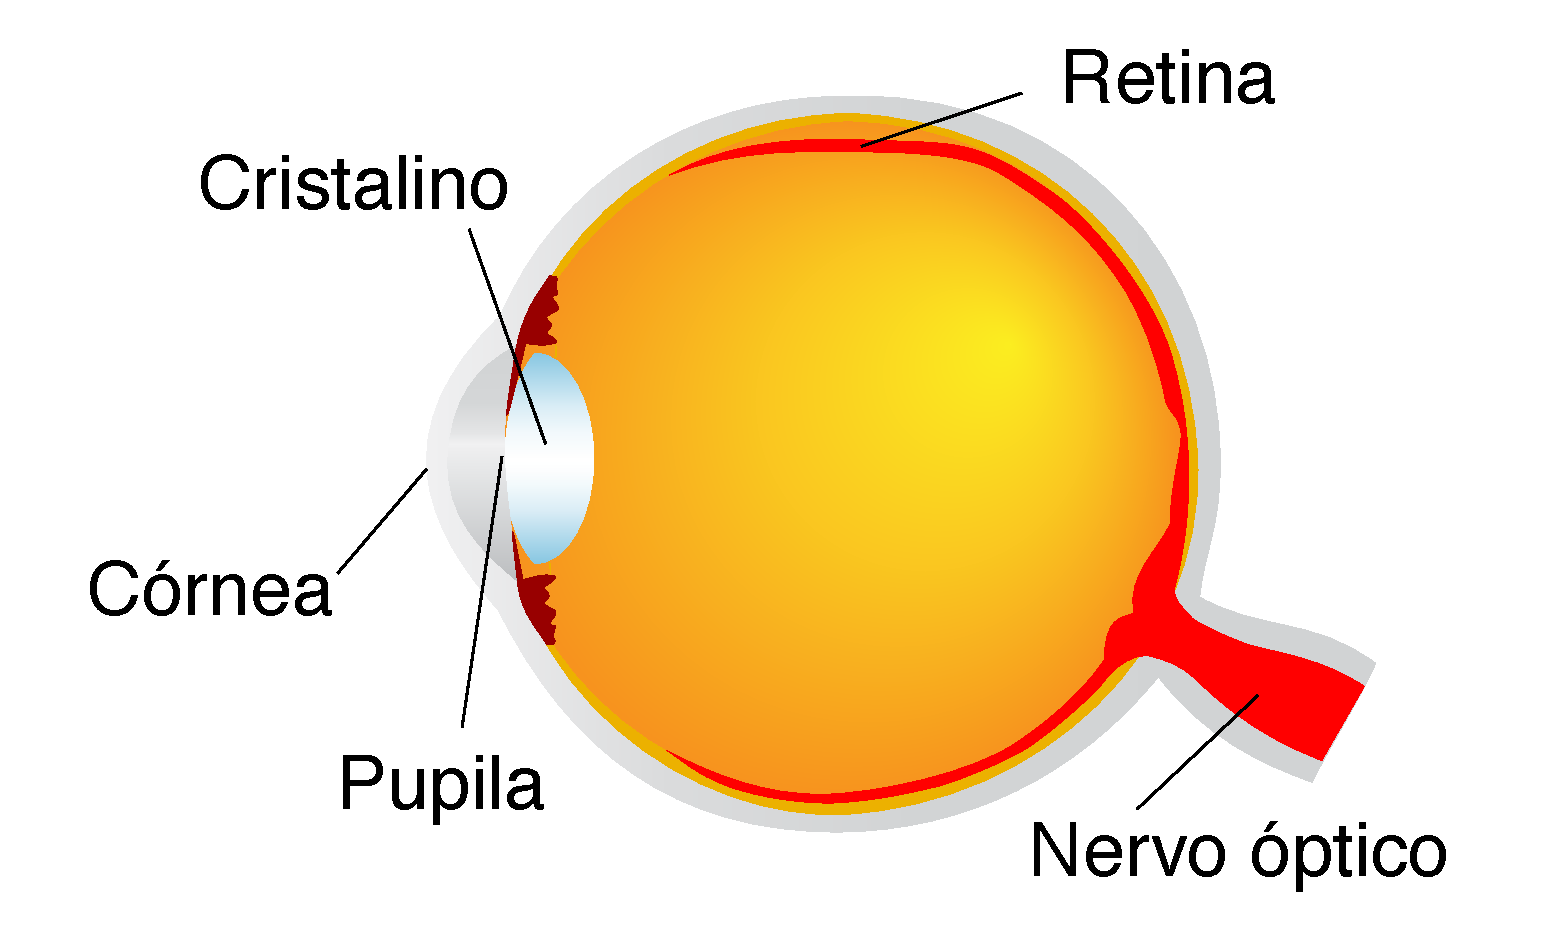
\includegraphics[width=0.5\textwidth]{olho-1}
	\caption{Diagrama dos principais elementos do olho humano. \label{fig:olho-1}} 
\end{figure}


Para uma pessoa com visão normal ou munida de correção adequada (óculos graduados ou lentes de contacto), os raios ópticos provenientes de um objecto no infinito\footnote{Para efeitos práticos, considera-se o infinito óptico qualquer distância superior a 5 m.} chegam paralelos ao olho e são focados na retina sem necessidade de esforço, ou seja, com o olho relaxado (Fig. \ref{fig:olho-2} à esq.). À medida que o objecto se aproxima do olho, é necessário os músculos ciliares aumentarem a curvatura da lente para criar uma imagem focada na retina -- a isto chama-se \emph{acomodação do olho}. O ponto mais próximo do olho para o qual a lente ainda consegue focar a imagem na retina é designado por \emph{ponto próximo} (Fig. \ref{fig:olho-2} à dir.) e considera-se igual a 0,25 m para uma visão normal padrão, valor que tem tendência a aumentar com a idade.

\begin{figure}
	[!htb]  \centering 
	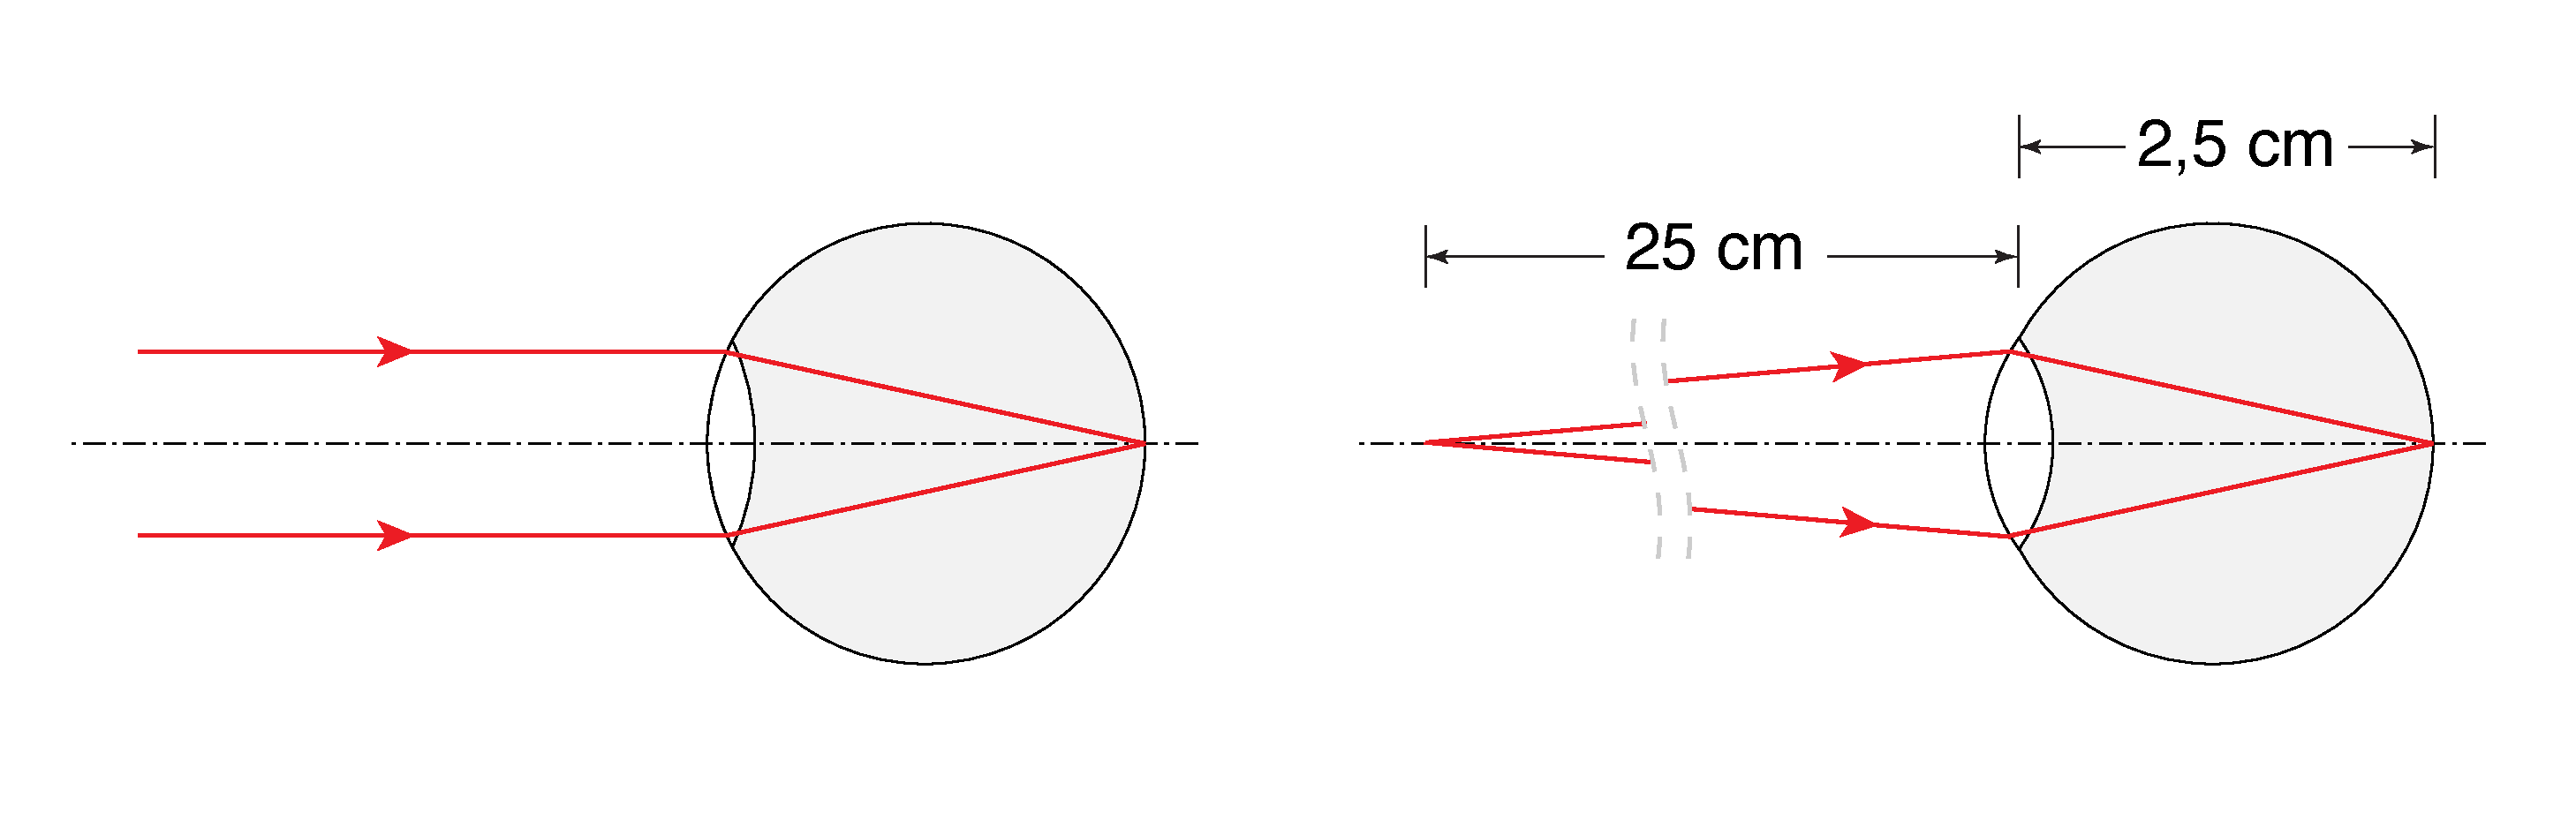
\includegraphics[width=0.9\textwidth]{olho-2}
	\caption{Esquema do olho no caso de objectos no infinito (esq.) e no ponto próximo (dir.). \label{fig:olho-2}} 
\end{figure}

O tamanho aparente dum objecto é determinado pelo tamanho que a imagem apresenta na retina. Mesmo sem variar o tamanho real do objecto, este pode ser visto maior se o aproximarmos do olho, porque o tamanho da sua imagem na retina é maior. A avaliação do tamanho da imagem na retina pode ser feita através da medição do ângulo $\theta$, que corresponde à inclinação dos raios principais do extremo da imagem (Fig. \ref{fig:olho-3}).

\begin{figure}
	[!htb]  \centering 
	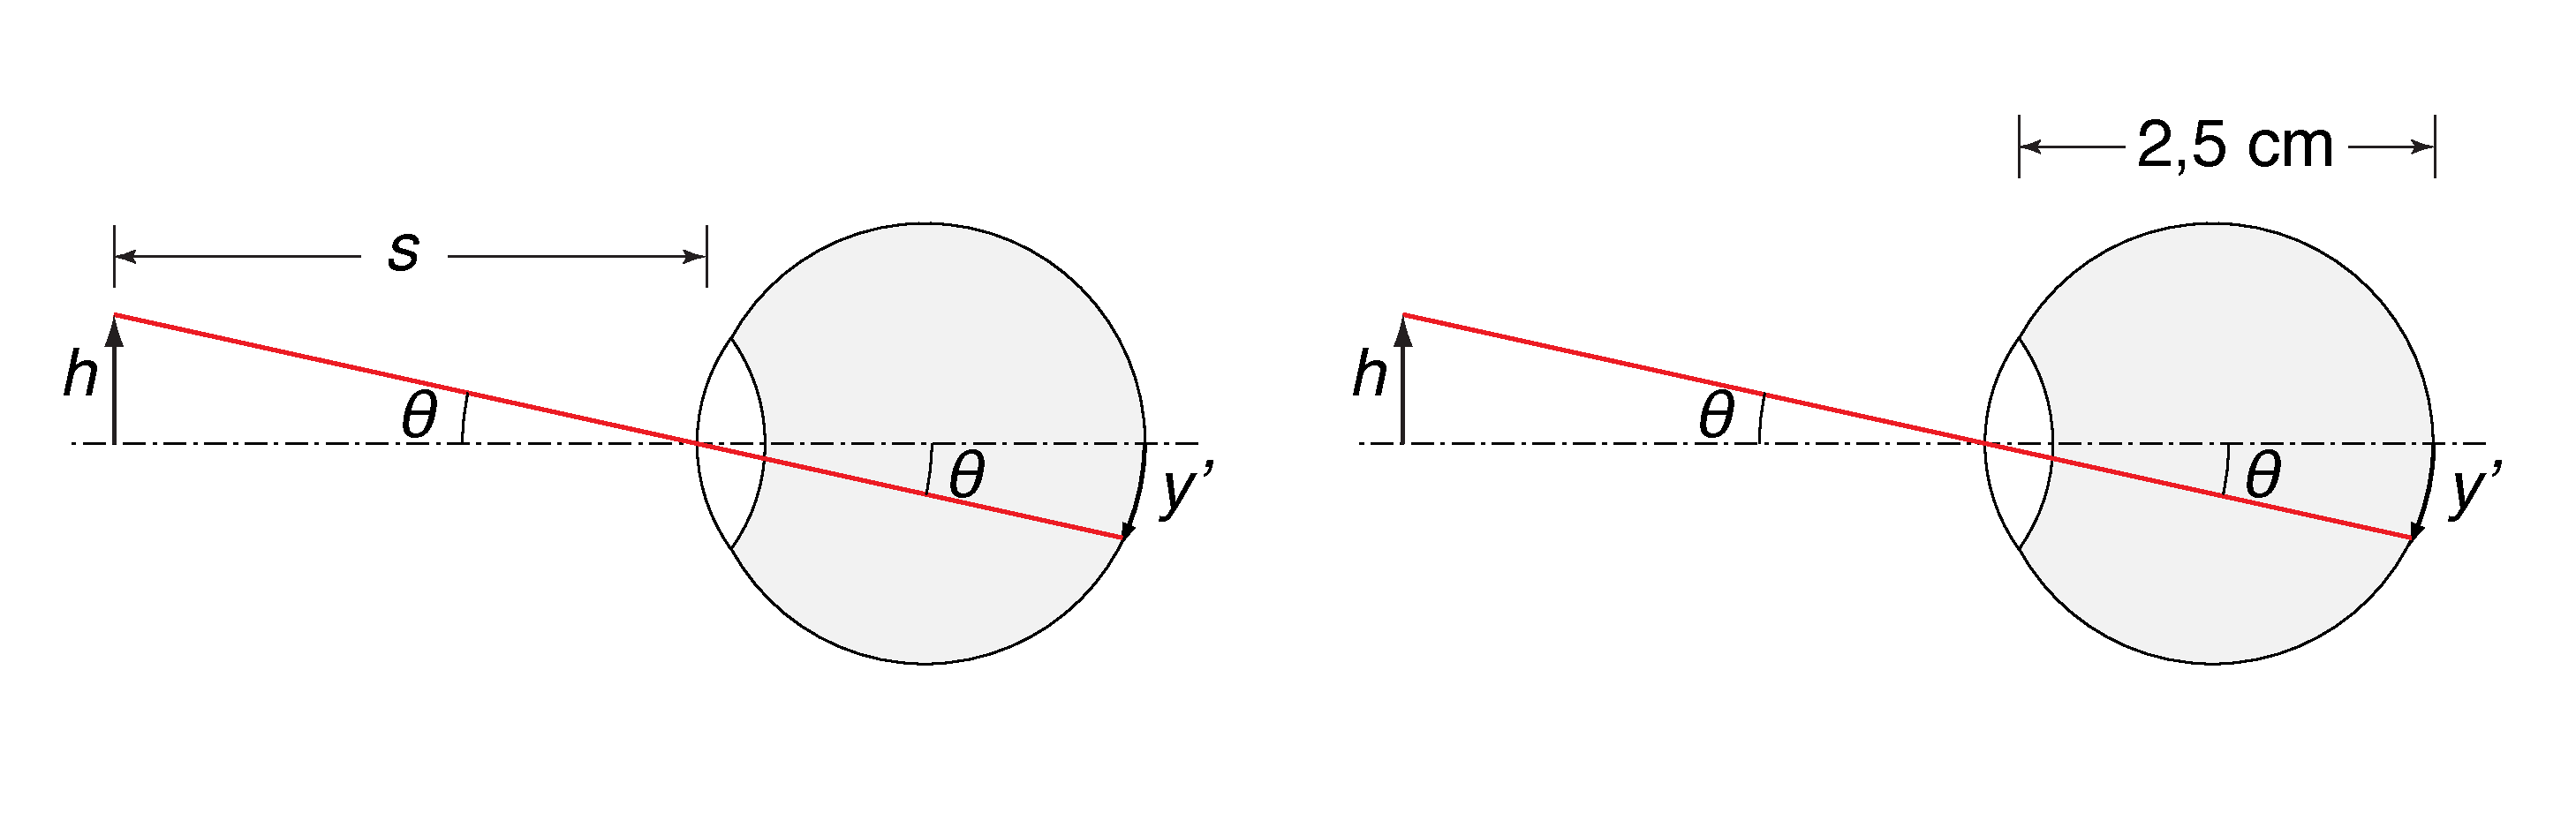
\includegraphics[width=0.9\textwidth]{olho-3}
	\caption{Formação de imagem na retina de um objecto de altura $h$ a uma distância $s$. \label{fig:olho-3}} 
\end{figure}

Considere-se um objecto com altura $h$ a uma distância $s$ do olho. Para o objeto podemos escrever $\tan\theta=h/s$. Para a imagem na retina, de altura $y'$, vem $\tan\theta = y' /$(2,5 cm). Na aproximação paraxial, ou seja de ângulos pequenos, podemos usar $\tan\theta \approx\theta$, e assim $\theta\approx h/s=y'/$(2,5 cm). Desta relação conclui-se que $y'$ é proporcional a $h$, tamanho do objecto, e inversamente proporcional à distância $s$ entre o objecto e o olho. 


O princípio dos instrumentos ópticos consiste no aumento do tamanho da imagem na retina, $y'$, permitindo assim visualizar objectos muito pequenos ou afastados. Do exposto acima, podemos concluir que a sua operação baseia-se na criação de uma imagem (real ou virtual) com um tamanho aparente maior que $h$ e/ou 
 a uma distância aparente inferior a $s$. Em qualquer dos casos, a imagem final produzida deverá estar situada além do ponto próximo, caso contrário não conseguirá ser focada.


%%%%%%%%%%%%%%%%%%%%%%%%%%%%%%%%%%%%%%%%%
\subsection{\sf Lupa}

A lupa simples é o instrumento óptico mais elementar. Consiste numa só lente convergente e permite aumentar o tamanho aparente do objecto, ou seja, o tamanho da imagem na retina. Sabendo que a maior imagem que se pode obter dum objecto com o olho desarmado é quando o objecto está no ponto próximo (Fig. \ref{fig:olho-4}), e dado que $y'_0$, tamanho da imagem na retina, é proporcional ao ângulo definido entre a altura do objecto $h_0$ e a sua distância ao olho, pode-se escrever a relação

\begin{equation}
\theta_0=h_0/0,25
\end{equation}

Na visão auxiliada pela lupa, esta é colocada perto do olho, e o objecto colocado a uma distância inferior ao foco. A imagem produzida pela lupa é virtual, ampliada e direita.

\begin{figure}
	[!tb]  \centering 
	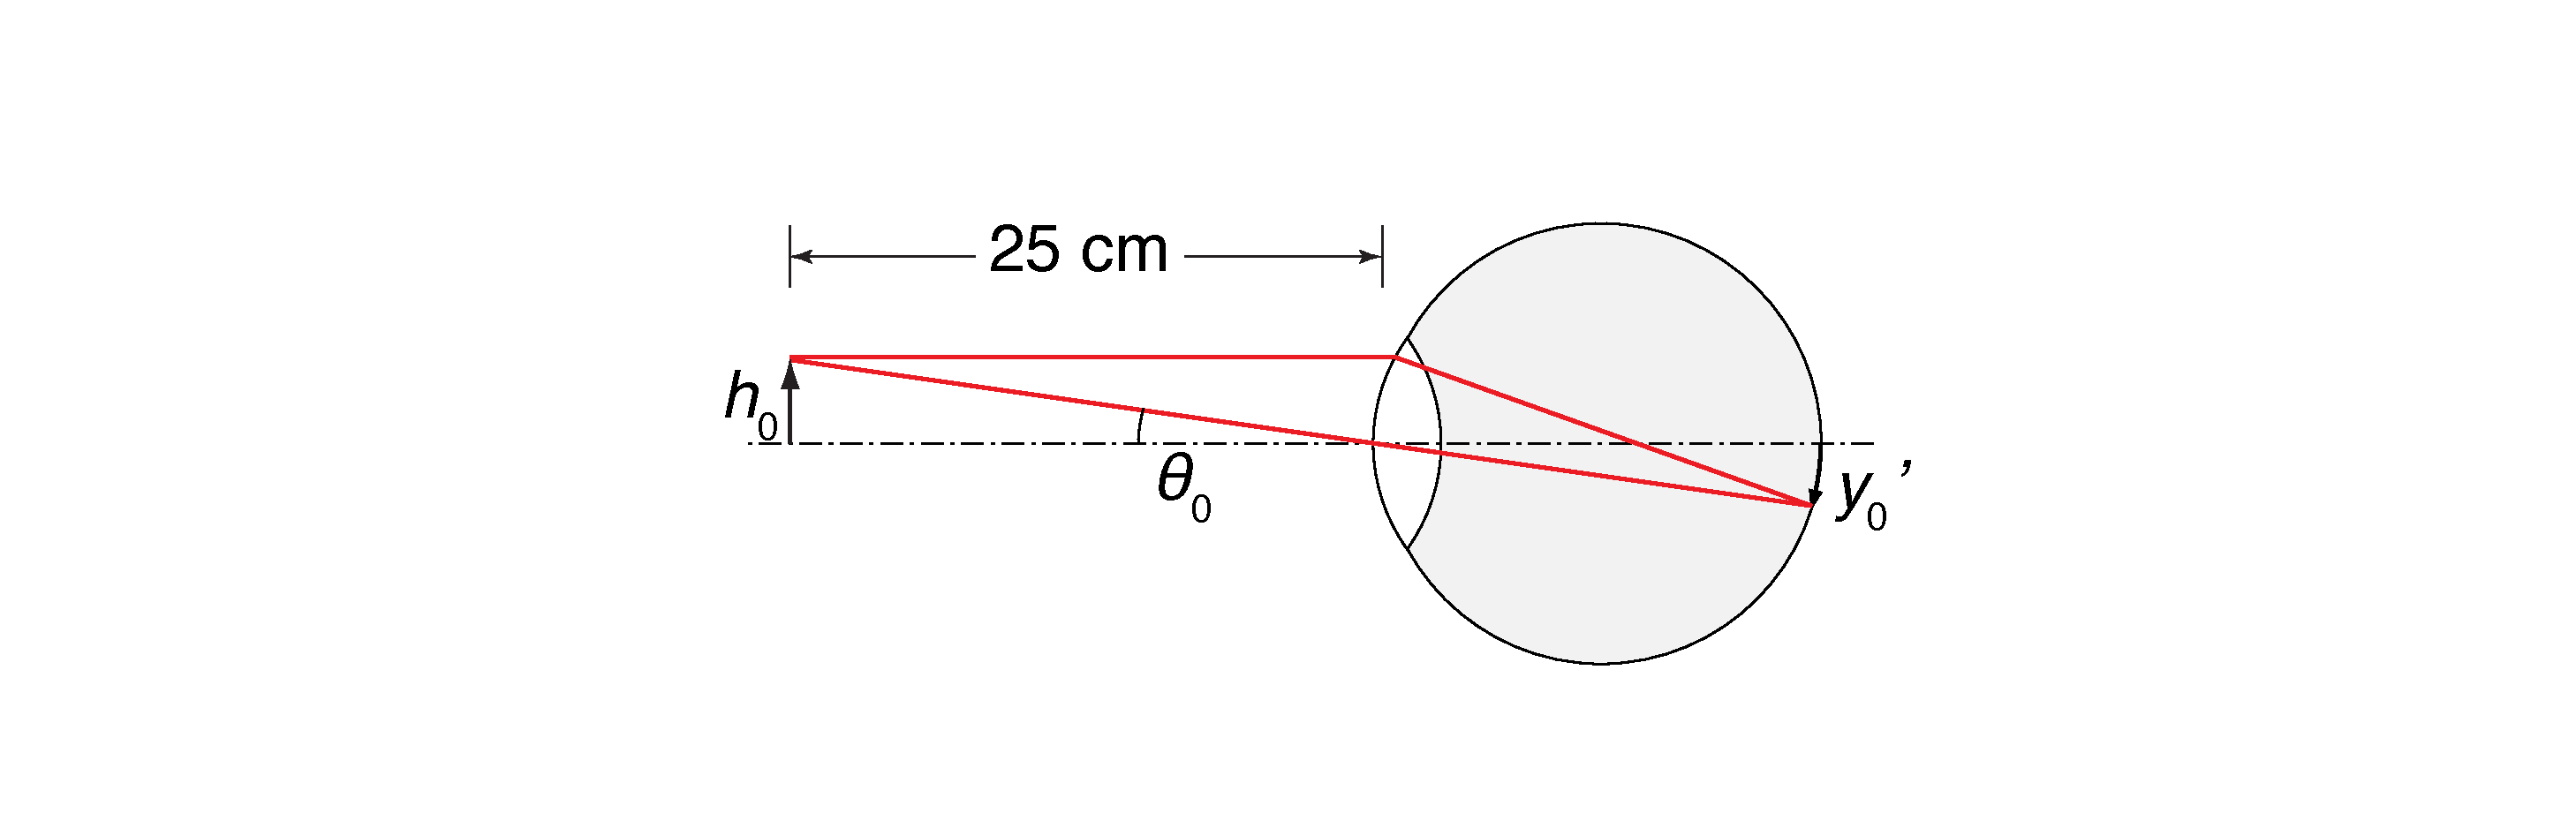
\includegraphics[width=0.8\textwidth]{olho-4}
		\caption{Objecto no ponto próximo visto pelo olho desarmado. \label{fig:olho-4}} 
\end{figure}



\begin{figure}
	[!b]  \centering 
	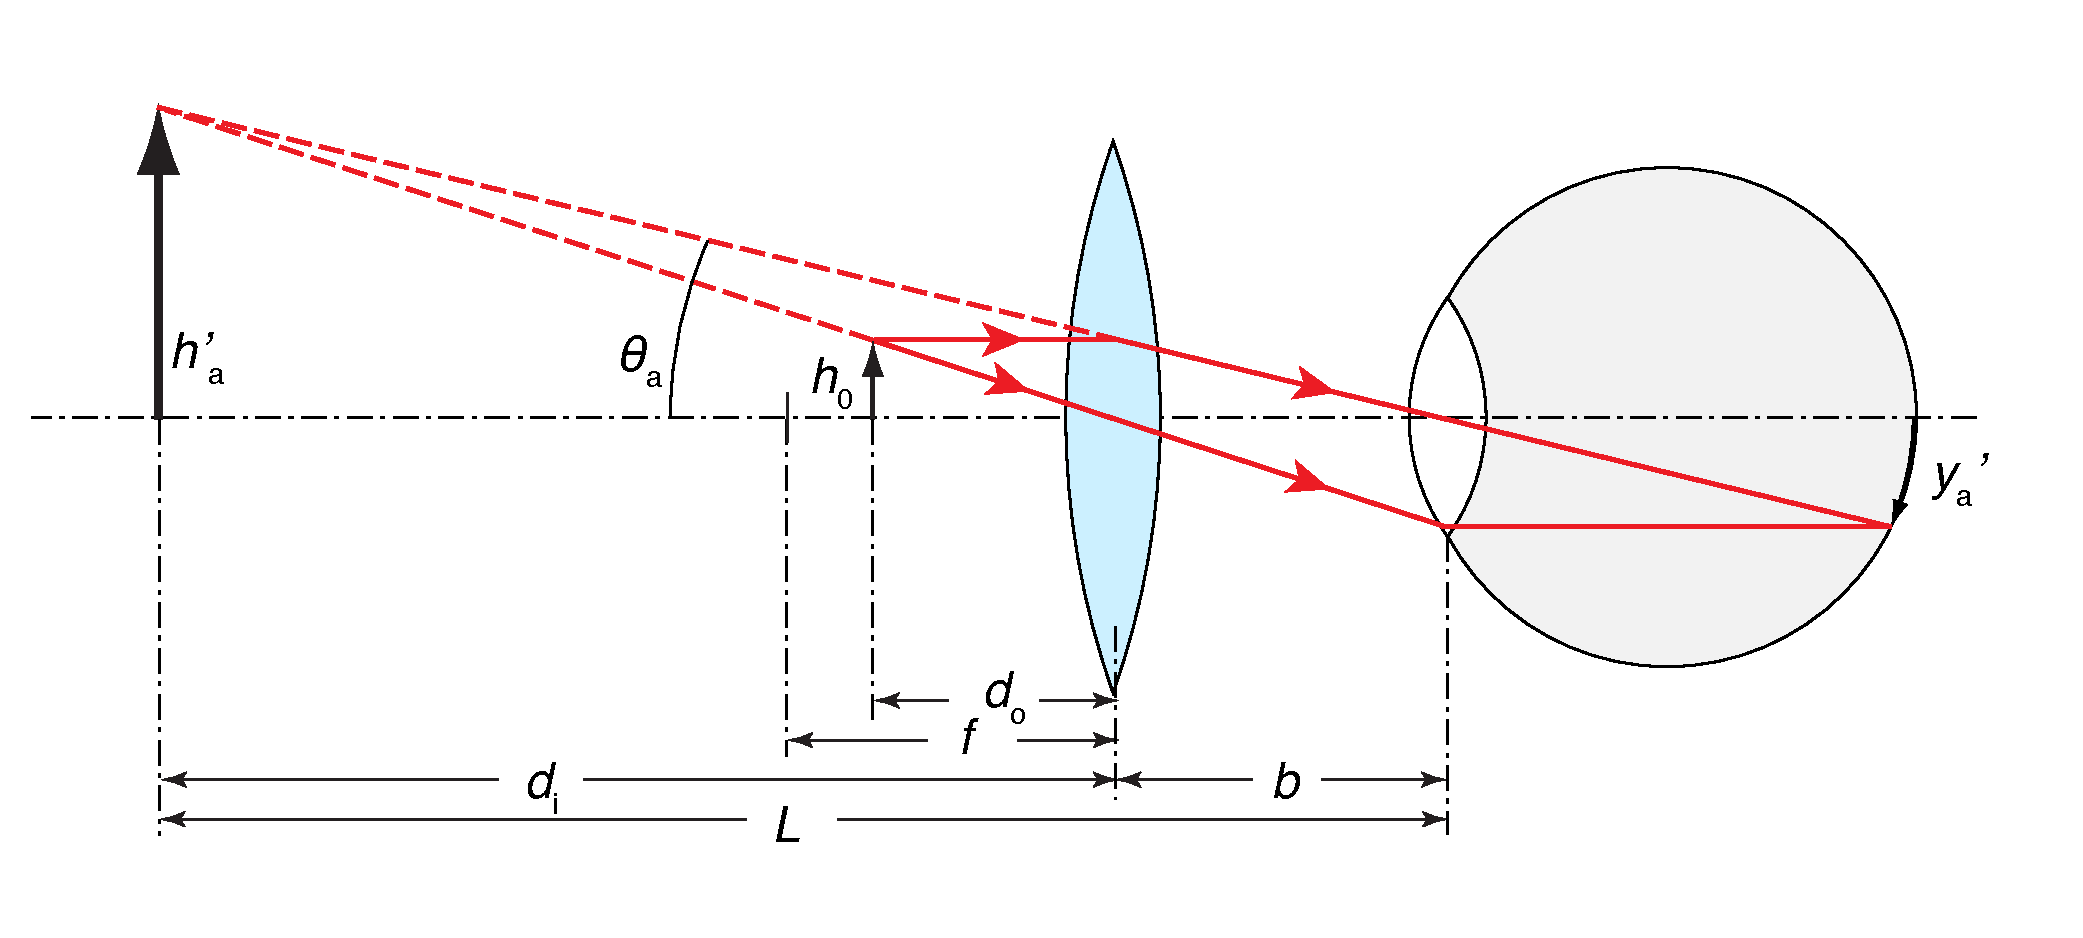
\includegraphics[width=0.8\textwidth]{olho-5}
	\caption{Formação de imagem com o auxílio de uma lupa a uma distância $b$ do olho. O objecto $h_0$ está a uma distância $d_O<f$ da lente, e a imagem (virtual) $h'_a$ aparenta estar a uma distância $d_i$ da lente e $L$ do olho. \label{fig:olho-5}} 
\end{figure}

\subsubsection{ \sf Ampliação angular}

A \emph{ampliação angular} $M_A$ dum instrumento óptico é determinada pela razão entre $y'_a$, dimensão da imagem na retina quando o objecto é visto através do instrumento (Fig. \ref{fig:olho-5}), e $y'_0$, dimensão da imagem na retina quando vista pelo olho desarmado e o objecto no ponto próximo. A razão entre os respectivos ângulos permite esse cálculo, isto é 

\begin{equation}
M_A=\frac{y'_a}{y'_0}=\frac{\theta_a}{\theta_0}
\end{equation}

Tirando partido da aproximação paraxial, temos $\tan\theta_a = h'_a / L \approx \theta_a$ e $\tan\theta_0 = h_0 / 0,25 \approx\theta_0$, portanto pode-se escrever a ampliação angular como:

\begin{equation}
M_A = \frac{h'_a/L}{h_0/0,25}=-\frac{d_i\,0,25}{d_0 L}= \frac{0,25}{L}\left(1-\frac{d_i}{f}\right) 
\end{equation}

onde na última igualdade se recorreu à equação dos focos conjugados. Como a distância à imagem é negativa, $d_i = - (L – b)$, obtém-se por fim

\begin{equation}
M_A = \frac{0,25}{L}\left(1+\frac{L–b}{f}\right)
\end{equation}

Da análise desta expressão pode-se dizer que a ampliação diminui se $L$ ou $b$ aumentam. Existem três casos particulares de ampliação:

\begin{enumerate}

\item  Se $b=f \to M_A = \frac{0,25}{f}=0,25D$, em que $D$ é a potência da lupa em dioptrias.

\item  Se $b=0\to M_A = 0,25\left(\frac{1}{L}+\frac{1}{f}\right)$.
Se $b= 0$ e também $L = 0,25 $ m (valor mínimo para $L$, uma vez que a imagem também deve poder ser focada correctamente pelo olho), então obtém-se para $M_A$ o valor máximo, igual a $M_A = 1+\frac{0,25}{f}= 1+0,25D$. Este caso corresponde a ter a lupa "encostada" ao olho, e a imagem aumentada surge à distância do ponto próximo.

\item  Se o objecto é colocado no foco ($d_O=f$), então a lupa forma a sua imagem no infinito $(L = \infty)$ e a ampliação é 
\begin{equation*}
M_A = \lim_{L\to\infty}\frac{0,25}{L}\left(1+\frac{L–b}{f}\right)= \frac{0,25}{f}=0,25D
\end{equation*}
Neste caso, o olho recebe raios paralelos e não necessita de fazer acomodação, o que é mais cómodo, e a ampliação apenas se reduz de uma unidade relativamente ao caso 2.
\end{enumerate}

Exemplo: uma lente com $D=10$ dioptrias tem uma distância focal $f=10$ cm, e para $L=\infty$ tem uma ampliação de $M_A=$2,5 vezes.


%%%%%%%%%%%%%%%%%%%%%%%%%%%%%%%%%%%%%%%%%
\subsection{\sf Microscópio composto}

O microscópio é o instrumento óptico empregado para observar objectos pequenos, colocados muito próximos do instrumento. Na sua forma mais simples, consiste em duas lentes convergentes. A lente mais próxima do objecto (\emph{objectiva}) tem uma distância focal $f_{obj}$, menor que a distância focal $f_{ocu}$ da lente mais perto do olho (\emph{ocular}) (Fig. \ref{fig:microscopio}).

\begin{figure}
	[!htb]  \centering 
	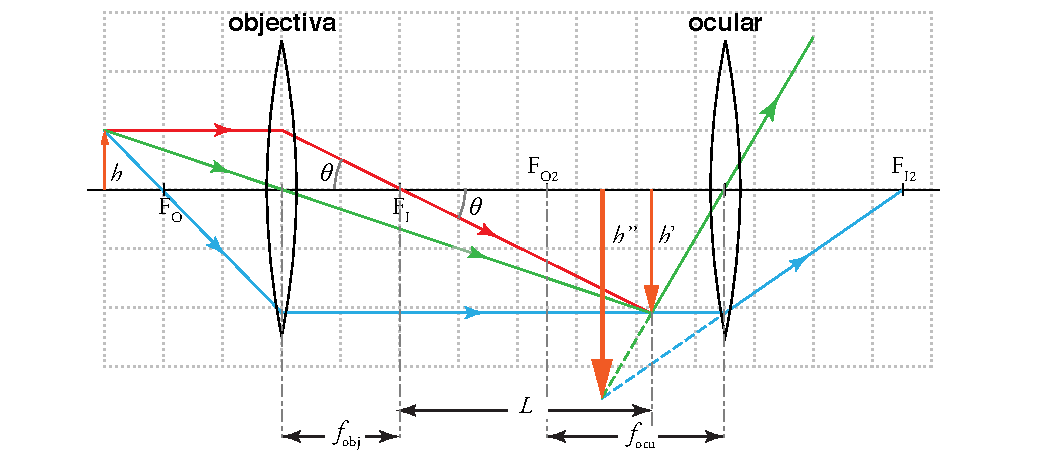
\includegraphics[width=0.9\textwidth]{microscopio}
		\caption{Formação de imagem num microscópio. \label{fig:microscopio}} 
\end{figure}

Um objecto de altura $h$ é colocado, em relação à objectiva, mais afastado do que o foco desta, produzindo uma imagem de tamanho $h'$ que é real, invertida e maior que o objecto. A objectiva produz assim uma imagem com \emph{ampliação transversal linear} $M_T$,\footnote{Conforme vimos atrás, para o caso de uma única lente esta ampliação é designada $A$.} dada por:

\begin{equation}
M_T=\frac{h'}{h} = -\frac{L\tan\theta}{f_{obj}\tan\theta}= -\frac{L}{f_{obj}}
\end{equation}

O sinal negativo indica que a imagem é invertida e, uma vez que é real, a imagem pode ser projectada sobre um alvo para se medir o seu tamanho.

A lente ocular é usada para aumentar a imagem formada pela lente objectiva. Assim, a ocular é colocada de modo a que a imagem $h'$ produzida pela objectiva (agora \emph{objecto virtual} da segunda lente) venha localizar-se a uma distância ligeiramente inferior ao seu foco $f_{ocu}$. Nesta condição, a ocular actua como uma simples lupa, que permite trazer o objecto $h’$ para uma distância mais curta do que o ponto próximo (0,25 m), e produz a imagem $h''$. A \emph{ampliação final} $M$ é dada pelo produto da ampliação transversal para a lente objectiva e a ampliação angular $M_A$ obtida para a lente ocular. No caso da lente ocular estar encostada ao olho, como é habitual num microscópio, estamos no caso $b=0$ e, das expressões anteriores para a ampliação linear e angular, obtemos

\begin{equation}
M = \frac{h''}{h}=M_T\times M_A.
\end{equation}




%%%%%%%%%%%%%%%%%%%%%%%%%%%%%%%%%%%%%%%%%%%%%%%%%%
\newpage
\section{\sf Procedimento experimental}


\subsection*{\sf Material}
Caixa de óptica equipada com
\begin{itemize}
\item calha graduada
\item fonte luminosa com lâmpada de incandescência linear
\item lentes convergentes e divergente
\item semi-cilindro de vidro acrílico
\item diafragmas
\item polaroides
\item suportes
\end{itemize}


\subsection*{\sf Trabalho preparatório} 
\begin{enumerate}
\item Preencha os objectivos do trabalho que irá realizar na sessão de laboratório. 
\item Preencha o quadro com as equações necessárias para o cálculo das grandezas, bem como as suas incertezas. 
\end{enumerate}
%%%%%%%%%%%%%%%%%%%%%%%%%%%%%%%%%%%%%%%%%%%%%%%%%%


\subsection{\sf  Determinação do índice de refracção dum vidro acrílico }
\subsubsection*{\sf Alinhamento}
\begin{enumerate}
\item Monte a fonte luminosa numa das extremidades da calha graduada e ligue a lâmpada.
\item Utilizando uma lente, obtenha  um  feixe  de  luz  branca  de  raios  paralelos. De que tipo de lente necessita?
\item Com os diafragmas, obtenha um feixe de luz estreito ($\approx$ 1 mm), alinhado com o eixo da calha graduada. Verifique que a espessura do feixe de luz se mantém tão constante quanto possível ao longo de toda a calha.
\end{enumerate}

\subsubsection*{\sf Face plana}
\begin{enumerate}
 \setcounter{enumi}{3}
\item Monte o suporte com o círculo graduado e o semi-cilindro  de  vidro  acrílico centrado, de modo a que o feixe de luz branca incida na sua superfície  plana.  Observe  e obtenha os ângulos de reflexão e de transmissão para vários valores dos ângulos do feixe incidente, à esquerda e à direita.  Registe medições  para, pelo  menos,  nove  valores  diferentes  do ângulo de incidência.
\item Represente as medições num gráfico e, a partir deste, determine por ajuste o índice de refracção do vidro acrílico.  Anexe o gráfico ao relatório.
\end{enumerate}

\subsubsection*{\sf Face cilíndrica}
\begin{enumerate}
 \setcounter{enumi}{5}
\item Rode o círculo graduado de modo a que o feixe de luz incida na  superfície cilíndrica do vidro acrílico. Repita  as  medidas  e  a  análise  dos  resultados. 
\end{enumerate}

\subsubsection*{\sf Ângulo-limite}
\begin{enumerate}
 \setcounter{enumi}{6}
 \item Estime o valor do índice de refracção a partir do ângulo limite de reflexão total. 
\item  Para o desvio à exatidão, considere como exato o valor médio das medições anteriores. 
\item Nas suas conclusões, compare os valores obtidos  para $n_{vidro}$ e a sua precisão 

\end{enumerate}

%%%%%%%%%%%%%%%%%%%%%%%%%%%%%%%%%%%%%%%%%%%%%%%%%%
\subsection{\sf Polarização da luz. Ângulo de Brewster}
\begin{enumerate}
\item Observe o efeito de interposição de dois filtros polarizadores, paralelos ou cruzados, no percurso de um feixe luminoso. 
\item Usando a mesma montagem do ponto anterior, polarize o feixe paralelamente ao plano
de incidência, orientando o eixo $0^\circ-180^\circ$ do filtro polarizador na vertical. 
\item A partir  do valor médio obtido para o índice de refracção (o que usou na secção anterior), calcule o valor "teórico" do ângulo de Brewster e verifique experimentalmente que, para esse valor, os raios reflectido e transmitido fazem 90$^\circ$ entre si. 
\item Para ângulos de incidência próximos do ângulo de Brewster, obtenha o  intervalo angular em que praticamente  se extingue o feixe reflectido. 
\end{enumerate}

%%%%%%%%%%%%%%%%%%%%%%%%%%%%%%%%%%%%%%%%%%%%%%%%%%
\subsection{\sf Distância focal de uma lente convergente ( $f  \approx$ 75 mm) }
 
\begin{enumerate}
\item Obtenha  um  feixe  de  luz  branca  de  raios  paralelos, usando a lente colimadora.
\item Seleccione a lente de distância focal mais curta e determine o seu valor pelo método directo.  Repita  a  experiência  duas  vezes,  colocando  a  lente 
noutra posição relativamente à lente de raios paralelos. 
\item Retire a lente colimadora e coloque o \emph{objecto} com mira no suporte da calha, iluminando-o directamente com a fonte luminosa. Coloque a mesma lente convergente a uma distância 150 mm $> d_O >$ 75 mm do objeto.

\item Com o écran plano, procure a posição correcta para obter uma \emph{imagem} focada.
Utilizando a equação dos focos conjugados, calcule de novo a d.f. da lente. 
\item Na folha quadriculada em anexo, desenhe um diagrama com o eixo óptico, o objecto e a lente convergente. Utilizando as aproximações paraxial e das lentes delgadas, desenhe a construção geométrica e obtenha a posição da imagem e a respectiva ampliação.

\item Medindo agora a imagem, determine a ampliação linear. Compare-a com a que podia  calcular pelas distância $d_O$  e $d_I$. 
\item Repita a experiência, colocando a lente noutra posição relativamente ao objecto.  
\item Compare o valor da distância focal com o obtido em (1) e estime a precisão envolvida em 
cada um dos métodos que utilizou. 
\end{enumerate}

%%%%%%%%%%%%%%%%%%%%%%%%%%%%%%%%%%%%%%%%%%%%%%%%%%
\subsection{\sf   Distância focal de uma lente divergente ( $f  \approx$ --150 mm) }
\begin{enumerate}
\item Associe  no  mesmo  suporte  a  lente  divergente  com  uma  convergente ($f  \approx$ 75 mm), de  forma a  que  o 
par se comporte como um sistema convergente (com $D\approx 10$ mm). Escolha uma distância ao objecto $D_O$ adequada e utilize esta montagem para determinar a distância focal da lente divergente.
\item Repita a montagem para uma diferente distância ao objecto. 
\end{enumerate}

%%%%%%%%%%%%%%%%%%%%%%%%%%%%%%%%%%%%%%%%%%%%%%%%%%

\subsection{\sf Microscópio composto}

\subsubsection*{\sf Material}
\begin{itemize}
\item Lente objectiva $f$ = 75 mm e lente ocular $f$ = 150 mm
\end{itemize}

\subsubsection*{\sf Medição da ampliação angular da ocular}
\begin{enumerate}
\item Monte um ecrã graduado (E1) na parte lateral exterior de um suporte a $d_i\approx 25$ cm da extremidade da calha, de modo a ficar no ponto próximo do observador. Este ecrã será a \emph{escala de referência}, desempenhando o mesmo papel que a escala na parede, no caso do telescópio.
\item Monte a lente ocular junto à mesma extremidade da calha, de modo a obter a condição $b\sim 0$ (verifique a Fig. \ref{fig:olho-5}). Calcule qual a distância $d_o$ dessa lente a que deverá colocar um objecto (altura $h_O$) de modo a que a sua imagem surja no ponto próximo. Use o valor obtido para determinar a ampliação angular (calculada).
\item Coloque outro ecrã graduado (E2) entre a lente e E1, próximo da posição $d_o$ calculada acima, de modo a conseguir visualizar simultaneamente (a) a escala de E2 através da lente, com o olho esquerdo, e (b) a escala de E1 com o olho direito.
\item Ajuste a posição de E2 até conseguir focar simultaneamente as imagens em ambos os olhos. Sobrepondo visualmente as duas escalas graduadas, meça o tamanho aparente $h'_a$ da imagem (virtual) de E2 e determine a ampliação angular $M_A$ da lente, usando a expressão adequada para esta configuração (ver Fig. \ref{fig:micro-composto})
% \item Na folha quadriculada em anexo desenhe um diagrama de traçado de raios, com o objecto a uma distância do foco igual $\approx f/5$. Obtenha a posição da imagem intermédia e da imagem final.
\end{enumerate}

\begin{figure}[h]
\begin{center}
	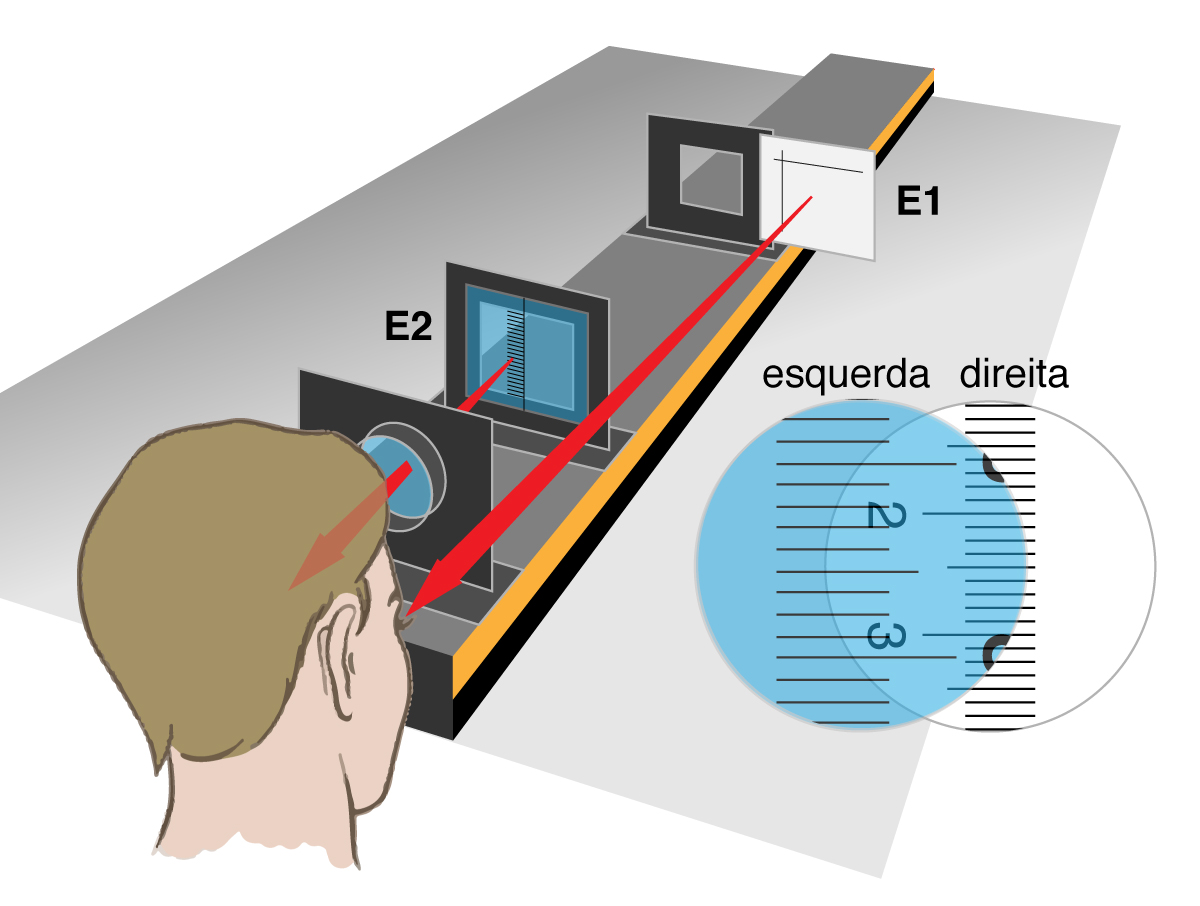
\includegraphics[width=0.45\textwidth]{micro-composto}
\caption{Esquema para a medição da ampliação angular da ocular.}
\label{fig:micro-composto}
\end{center}
\end{figure}

\subsubsection*{\sf Medição da ampliação linear da objectiva}
\begin{enumerate}[resume]
\item Mantendo a ocular montada e usando como referência a Fig. \ref{fig:microscopio}, junte uma objectiva e um objecto (um écran graduado iluminado). Escolha uma altura $h_0$ adequada.
\item Se necessário, ajuste a objectiva para observar uma imagem focada através da ocular.
\item Com um ecrã auxiliar, observe a imagem intermédia $h’$ e meça a sua ampliação.
\item Calcule a ampliação final do microscópio composto.
\end{enumerate}
\HRule
%%%%%%%%%%%%%%%%%%%%%%%%%%%%%%%%%%%%%%%%%%%%%%%%%
%%%%%%%%%%%%%%%%%%%%%%%%%%%%%%%%%%%%%%%%%%%%%%%%%
%%%%%%%%%%%%%%%%%%%%%%%%%%%%%%%%%%%%%%%%%%%%%%%%%
%%%%%%%%%%%%%%%%%%%%%%%%%%%%%%%%%%%%%%%%%%%%%%%%%
%%%%%%%%%%%%%%%%%%%%%%%%%%%%%%%%%%%%%%%%%%%%%%%%%
%%%%%%%%%%%%%%%%%%%%%%%%%%%%%%%%%%%%%%%%%%%%%%%%%
%%%%%%%%%%%%%%%%%%%%%%%%%%%%%%%%%%%%%%%%%%%%%%%%%
%%%%%%%%%%%%%%%%%%%%%%%%%%%%%%%%%%%%%%%%%%%%%%%%%
%%%%%%%%%%%%%%%%%%%%%%%%%%%%%%%%%%%%%%%%%%%%%%%%%
%%%%%%%%%%%%%%%%%%%%%%%%%%%%%%%%%%%%%%%%%%%%%%%%%

\chapter{\huge{Espectroscopia e efeito fotoeléctrico}}
\large {\bf {Riscas espectrais e medição da constante de Planck}}\\
	\HRule %[0.5cm]

%\newpage
\section{\sf Objectivos do trabalho}
Pretende-se com este trabalho investigar e fazer uso de várias propriedades da óptica ondulatória, nomeadamente da separação angular das riscas de emissão de lâmpadas espectrais. Utilizando um goniómetro, iremos proceder à medição dos ângulos de refracção de um prisma e de difracção de uma rede, em função do comprimento de onda. A separação das riscas espectrais será também usada para verificar o efeito fotoeléctrico e obter uma medição da constante de Planck.

Como objetivo associado, pretende-se tomar conhecimento e aprender a manusear e a realizar medidas correctamente  com um instrumento óptico de precisão, o \emph{goniómetro}. Este instrumento permite medir ângulos de desvio, por reflexão ou refracção de feixes de raios paralelos, com uma resolução inferior a um minuto de grau.

%%%%%%%%%%%%%%%%%%%%%%%%%%%%%%%%%%%%%%%%
\section{\sf Conceitos fundamentais}
\subsection{\sf Desvio da luz por um prisma}
Em óptica designa-se por \emph{prisma} um sólido transparente em forma de prisma triangular, homogéneo e isotrópico, caracterizado pelo ângulo do vértice $\alpha$ e pelo índice de refração $n$. Quando colocado no percurso de um feixe luminoso incidente, o prisma produz um desvio angular no feixe emergente que depende do ângulo de incidência e do comprimento de onda $\lambda$ (Fig. \ref{fig:prisma1}). Na região da luz visível, verifica-se que os comprimentos de onda mais curtos são mais desviados, ou seja, a luz violeta é mais desviada que a luz vermelha.

\begin{figure}[htb]  \centering 
	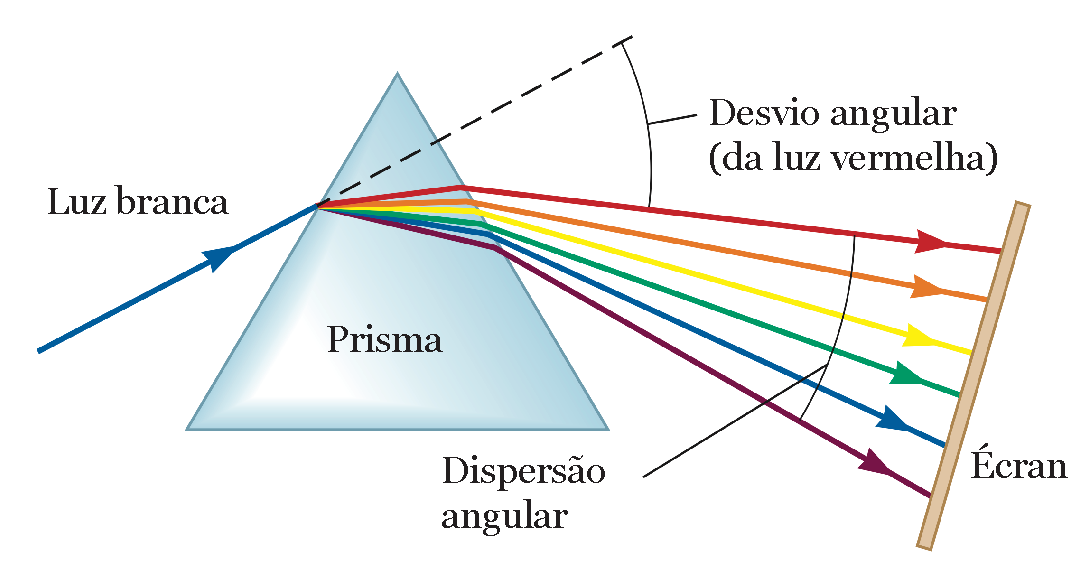
\includegraphics[width=0.5\textwidth]{prisma1.pdf}
	\caption{Desvio da luz por um prisma: um feixe de luz branca é desviado da sua direcção original de um ângulo que depende do ângulo de incidência e do comprimento de onda. \label{fig:prisma1}} 
\end{figure}

A Fig. \ref{fig:prisma2} mostra este processo em maior detalhe. Um raio luminoso (traço vermelho contínuo) incide na face esquerda do prisma segundo um ângulo $i_1$ (em relação à normal à superfície) e é refractado internamente segundo um ângulo $t_1$. Após se propagar dentro do prisma, o raio incide na face direita segundo um ângulo $i_2$ e é refractado para o exterior segundo um ângulo $t_2$. À diferença entre a direcção original e a desviada chamamos \emph{desvio angular} $\delta(\lambda)$. Pode provar-se que a função $\delta(\lambda)$ apresenta um ponto estacionário (i.e., derivada nula) que é um mínimo se $n > 1$. Mostra-se também que, nessa situação, as direções dos dois feixes são igualmente inclinadas em relação às faces do prisma, i.e.  o ângulo de incidência $i_1$ é igual ao ângulo de transmissão emergente $t_2$. Nesse caso, o índice de refração, $n$, pode ser calculado simplesmente através da expressão seguinte: 

\begin{equation}
	\label{eq:desviomim}
	n= \frac{\sin \left( \frac{\alpha+ \delta_{min}}{2} \right) } {\sin \left(  \frac{\alpha}{2} \right)}  
\end{equation}
em que $\alpha$ e  $\delta_{min}$ são o ângulo do vértice do prisma e o \emph{ângulo de desvio mínimo} referido, respectivamente. Uma vez que o índice de refracção depende $\lambda$, podemos concluir que também o valor de $\delta_{min}$ vai depender do comprimento de onda: diferentes cores vão apresentar diferentes desvios mínimos. Este princípio permite, através da medição do desvio mínimo $\delta_{min}(\lambda)$ para vários comprimentos de onda, determinar por ajuste a variação do índice de refracção do material do prisma.


\begin{figure}[htb]  \centering 
	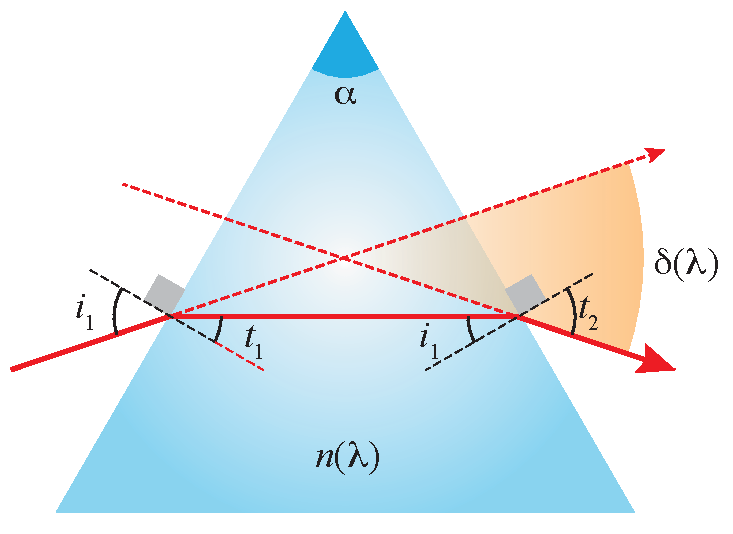
\includegraphics[width=0.5\textwidth]{prisma2.pdf}
	\caption{Definição de \emph{ângulo de desvio} $\delta(\lambda)$. A luz viaja da esquerda para a direita através de um prisma de índice de refracção $n(\lambda)$ e ângulo de vértice $\alpha$. \label{fig:prisma2}} 
\end{figure}

\subsection{\sf Rede de difracção}
Uma rede de difracção é um componente óptico com uma estrutura microscópica periódica – por exemplo, pode ser composto por fendas paralelas (linhas) com espaçamentos da ordem do micrómetro. Caracteriza-se a rede pelo número $N$ de linhas por mm, que é assim da ordem de várias centenas, ou mesmo superior. Tal como o prisma, a rede tem a propriedade de desviar a luz incidente em função do ângulo de incidência e do comprimento de onda $\lambda$, só que duma forma muito mais apreciável. Um raio de luz de c.d.o. $\lambda$ que incida com um ângulo $\theta_i$ (relativamente à normal) numa rede de difracção com $N$ linhas/mm é difractado segundo um ângulo $\theta_d$, de acordo com
\begin{equation}
\sin \theta_i+\sin\theta_d=m \lambda N
\end{equation}
em que $m$ é a \emph{ordem de difracção}. A Fig. \ref{fig:rede1} ilustra a difracção para o caso em que o ângulo de incidência é nulo, isto é, o feixe incide segundo a normal à superfície. O feixe central, não desviado, é considerado como $m=0$, enquanto que à esquerda e direita surgem simetricamente as ordens $m=\pm 1, \pm 2$, etc., cada vez menos intensas.

\begin{figure}[!t]  
\centering 
	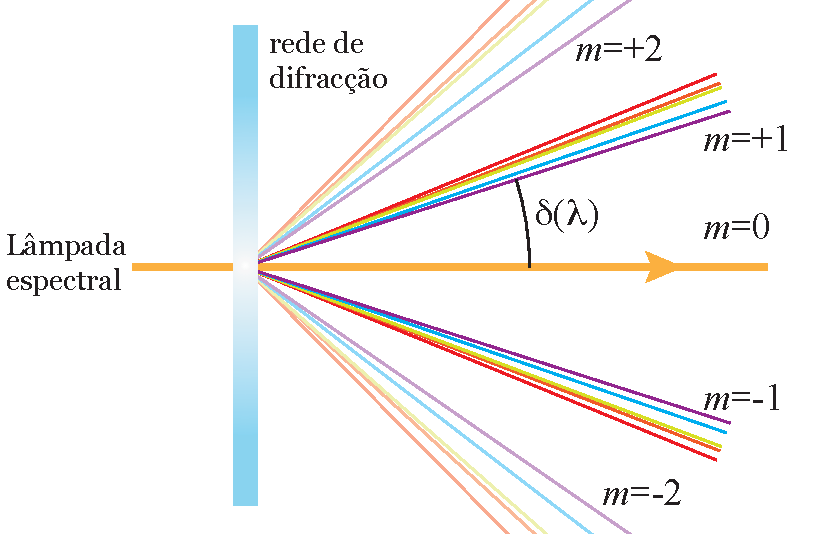
\includegraphics[width=0.5\textwidth]{rede1}
	\caption{Desvio da luz por uma rede de difracção, com o surgimento de ordens de difracção. \label{fig:rede1}} 
\end{figure}


\section{\sf Goniómetro de Babinet}
O goniómetro é um instrumento que permite medir ângulos com grande precisão, e muito utilizado em óptica. O goniómetro de Babinet tem uma base central quase cilíndrica com uma plataforma que roda em torno do eixo vertical daquela, na qual é colocado o elemento dispersor da luz (prisma ou a rede de difracção) (Figura \ref{fig:goniometer}). 

O goniómetro vem equipado com dois elementos ópticos: um \emph{colimador} e uma \emph{luneta}. Ambos estão montados radialmente, o colimador fixo e a luneta podendo rodar em torno do eixo da base (Figura \ref{fig:babinet}). As posições angulares da plataforma (e, portanto, do prisma ou da rede) e da luneta podem ser lidas num limbo graduado por intermédio de nónios solidários, respetivamente com a plataforma e a luneta. Existem dois parafusos micrométricos, cada um associado a cada um dos nónios, que permitem com facilidade regular e fazer leituras das posições angulares, com resolução de $30''$ (meio minuto de grau).

\begin{figure}  
\centering 
	\includegraphics[width=0.75\textwidth]{goniometer}
	\caption{Goniómetro de Babinet . \label{fig:goniometer}} 
\end{figure}

O \emph{colimador} é constituído por dois tubos cilíndricos concêntricos que se podem deslocar axialmente. Um deles possui uma fenda rectilínea, de largura variável por um parafuso, e que deve ser colocada na vertical (pode utilizar a mira da ocular depois de regulada) e encostada à fonte luminosa. O outro tubo tem no extremo oposto (virado para a plataforma) uma lente convergente, $L_C$. O objectivo deste conjunto é produzir um feixe de raios paralelos na região da plataforma onde se coloca o prisma, rede, ou espelho. A fenda, se for relativamente estreita, vai funcionar como objecto linear e dar origem às riscas observadas.

\begin{figure}
	\centering 
	\includegraphics[width=0.65\textwidth]{Babinet}
	\caption{Esquema do goniómetro. FL -- fonte luminosa, F -- fenda, Lc -- lente convergente, Pt -- plataforma, Esc -- escala fixa na base, NL -- nónio acoplado ao suporte da luneta, NP -- nónio acoplado ao suporte do prisma, Obj -- objetiva, Oc -- ocular, Ret -- retículo.
	\label{fig:babinet}} 
\end{figure}

A \emph{luneta} é constituída por dois elementos ópticos, uma lente convergente e uma ocular munida de retículo (dois fios cruzados perpendicularmente). A primeira lente produz no seu plano focal a imagem intermédia da fenda, que é projectada no plano do retículo e ampliada pela ocular. A ocular é regulada pelo observador, de modo a ver uma imagem focada da fenda.

\subsection{\sf Leitura de valores no goniómetro}
O goniómetro tem uma escala central, fixa e solidária com a base, com valores entre $0^\circ$ e $360^\circ$. Entre cada grau há três divisões, ou seja, a escala está dividida em intervalos de 1/3 grau = 20 minutos de arco (20') (Fig. \ref{fig:gonio-nonio1}). Existem duas escalas rotativas com um nónio: a de cima está unida à plataforma e permite ler o ângulo de incidência, a de baixo está ligada à luneta e permite ler o ângulo de desvio. Estes ângulos são relativos, por exemplo, à direcção do feixe de luz sem sofrer desvio. Ambas as escalas móveis estão equipadas com nónios de 40 divisões, aumentando assim a precisão da leitura para 20'/40=0.5', ou seja, 30 segundos de arco. O uso desta precisão é facultativo nas medições feitas com a rede (dada a amplitude dos ângulos de desvio) mas é obrigatório para medições com o prisma.

\begin{figure}
	\centering 
	\includegraphics[width=0.5\textwidth]{gonio-nonio1}
	\caption{Escala fixa (menor divisão: 20') e escala rotativa, com nónio, do goniómetro.
	\label{fig:gonio-nonio1}} 
\end{figure}

O procedimento para ler um dado valor usando o(s) nónio(s) é semelhante ao usado na craveira (Fig. \ref{fig:gonio-nonio2}). Começa-se por ler na escala fixa, com a maior precisão possível, o valor imediatamente à esquerda da linha do zero do nónio. A esse valor acrescenta-se o valor indicado pela divisão cuja linha coincide em ambas as escalas. Dado o tamanho diminuto destas divisões, é aconselhável fazer a leitura com o auxílio de uma lupa, ou registar a leitura através de fotografia digital (Fig. \ref{fig:gonio-lente}).

\begin{figure}[h]
	\centering 
	\includegraphics[width=0.5\textwidth]{gonio-nonio2}
	\caption{Exemplo de leitura no goniómetro. Escala fixa: $123^\circ+40'$; nónio: 6,5'. Valor da leitura: $123^\circ46,5'$
	\label{fig:gonio-nonio2}} 
\end{figure}

\begin{figure}[h]
	\centering 
	\includegraphics[width=0.4\textwidth]{gonio-lente}
	\caption{Registo em fotografia digital auxiliado por lente da leitura do goniómetro.
	\label{fig:gonio-lente}}
\end{figure}

Por outro lado, o valor que é lido nas duas escalas do goniómetro – escala da plataforma e escala da luneta – não coincide necessariamente com o ângulo de incidência ou o ângulo de desvio, respectivamente, o que pode levar a confusão no registo dos valores. A Fig. \ref{fig:babinet3} ilustra esta situação para o caso da refracção no prisma. Por uma questão de consistência, iremos utilizar a seguinte convenção:

\begin{itemize}
\item Os ângulos de incidência e transmissão nos componentes ópticos, relativamente às suas superfícies, são designados $\theta_i$ e $\theta_t$ respectivamente
\item Os ângulos lidos na escala da plataforma e na escala da luneta são designados $\phi_i$ e $\phi_t$ respectivamente; 
\item O ângulo lido na escala da luneta na ausência de componente óptico é $\phi_{i0}$; nessa configuração a luneta encontra-se perfeitamente alinhada com o colimador
\end{itemize}

De novo considerando a Fig. \ref{fig:babinet3}, para o caso do prisma pode deduzir-se a seguinte relação entre $\phi_{i0}$, $\phi_t$ e o ângulo de desvio:
\begin{equation}
\delta=|\phi_{i0}-\phi_t |
\end{equation}

\begin{figure}[h]
	\centering 
	\includegraphics[width=0.6\textwidth]{Babinet3}
	\caption{Identificação dos diversos ângulos na refracção da luz por um prisma.
	\label{fig:babinet3}} 
\end{figure}




\newpage


\section{\sf Efeito fotoeléctrico}
O efeito fotoeléctrico era já conhecido no final do séc. XIX, com a emissão  de partículas carregadas da superfície de um metal quando iluminadas por luz intensa. Verificou-se também que a energia destas partículas, que mais tarde foram identificadas por electrões, não dependia da intensidade da luz incidente mas sim do  seu comprimento de onda, $\lambda$.  A explicação correcta do efeito fotoeléctrico foi proposta em 1905 por Albert Einstein\footnote{Pela qual recebeu o prémio Nobel em 1921.} baseada na teoria de Max Planck\footnote{Teoria Quântica da luz, pela qual recebeu o prémio Nobel em 1918.} da emissão-absorção da luz. Para ambos, a luz seria formada pela emissão de  corpúsculos (\emph{quanta}), que se batizaram como \emph{fotões}, cada um com energia $E$  dada por $E = h \nu$, em que $h$ é apropriadamente a \emph{constante de Planck} e $\nu$ a frequência da luz ($\nu=c/\lambda$).  De acordo com esta teoria corpuscular da luz, quando um fotão incide sobre a superfície de um metal é absorvido por um átomo, e a sua energia é depositada num dos electrões de valência.
% A estes electrões tem de ser depositada uma energia para que se libertem da rede metálica. 
 Se o fotão incidente tiver mais energia que um dado limiar ($W_0$ - \emph{Work function}, característica de cada metal), o  electrão é libertado da rede metálica e emitido do sólido com uma energia cinética $K_e = h\nu - W_0$.
A intensidade da luz determina assim o \emph{número de fotolectrões} emitidos, mas não a sua energia!

A Fig. \ref{fig:pe-effect} representa esquematicamente o efeito. Os fotões incidentes, de energia $h\nu$, libertam electrões próximos da superfície do sólido. Note-se que se a energia do fotão incidente não for suficiente (i.e. se $E_f < W_0$) não há emissão de fotoelectrões.

\begin{figure}[htb] 
	\centering 
	\includegraphics[width=0.65\textwidth]{pe-effect.pdf}
	\caption{Ilustração do efeito fotoeléctrico} \label{fig:pe-effect}
\end{figure}

A constante de Planck pode ser determinada expondo a superfície de um metal a luz monocromática, caracterizada por um comprimento de onda $\lambda=c /\nu$ fixo e medindo a energia cinética máxima dos fotoelectrões emitidos. A Fig.~\ref{fig:plack_exp} representa esquematicamente uma montagem experimental para a realização desta experiência.

\begin{figure}[htb] 
	\centering 
	\includegraphics[width=0.5\textwidth]{planck_exp.pdf}
	\caption{Diagrama esquemático da experiência do efeito fotoeléctrico. V - fonte de tensão (potencial retardador); C - condensador; K - cátodo; A - ânodo; F - filtro óptico.} \label{fig:plack_exp}
\end{figure}
A luz incide na superfície de um sólido metálico, designado \emph{cátodo} (K), através de um \emph{ânodo} (A) anelar ou transparente. 
Como cátodo, é normalmente utilizado um metal alcalino (potássio, sódio ou cádmio)  pois neste caso os electrões de valência estão fracamente 
ligados ao núcleo (i.e. têm uma baixa função trabalho $W_0$). Como ânodo, utiliza-se por exemplo a platina (Pt). 
O ânodo recebe parte dos fotoelectrões emitidos, dando origem a uma corrente $I_f$ no circuito exterior. 
Se aplicarmos um potencial eléctrico retardador $V$ entre o ânodo e o cátodo a fotocorrente decresce, pois os fotoelectrões terão de vencer uma barreira de potencial electrostática $U=e V$, onde $e$ é a carga do electrão. 
Para uma dada tensão crítica $V_s$ (potencial de paragem), deixa de existir fotocorrente. 
%Neste caso, mesmo os electrões mais fracamente ligados e que assim têm as maiores energias cinéticas, são parados. 

%$I_f=C\frac{dq}{dt}$
Experimentalmente, pode usar-se uma fonte de tensão externa para aplicar o potencial de paragem. Mais simplesmente, pode usar-se um condensador para acumular a carga ($q=C V$) transportada pela própria corrente dos fotoelectrões (Fig.~\ref{fig:plack_exp}), aumentando gradualmente a diferença de potencial $V$, até se atingir o valor $V_s$, para o qual a corrente é  auto-eliminada. Mas neste caso, é necessário utilizar um voltímetro de impedância de entrada muito elevada ($> 10\textrm{ M}\Omega$) ou um amplificador electrónico de instrumentação, que é o caso da nossa montagem experimental.
 Após medir o potencial de paragem, podemos assim escrever:\footnote{Na realidade a função de trabalho tem de ser corrigida pelo potencial de contacto entre os dois metais, $W=W_0 - \phi$, o que naturalmente não é importante para a determinação da constante de proporcionalidade.}
\begin{equation}
	\label{eq:energia}
	e\,V_s= K_e^{max}= h \nu - W_O
\end{equation}
Medindo o potencial de paragem sucessivamente para luz incidente de várias frequências, podemos então fazer o gráfico de $V_s\; vs. \;\nu$. Este gráfico deverá aproximar-se de uma recta de declive $h/e$ e ordenada na origem  $-W_0/e$ (ver exemplo na Fig. \ref{fig:pe-graph}).


\begin{figure}[htb] 
	\centering 
	\includegraphics[width=0.65\textwidth]{pe-graph.pdf}
	\caption{Exemplo da determinação de $h$ pelo efeito fotoeléctrico} \label{fig:pe-graph}
\end{figure}

Desde a redefinição do Sistema Internacional de Unidades de 2019, a constante $h$ é definida como tendo um valor exacto: $h=6.626\,070\,15 \times 10^{-34}\ \textrm{J}\cdot \textrm{s}$ ou, em unidades de electrão-volt, $h=4.135\,667\,696\times 10^{-15}\,\textrm{eV}\cdot\textrm{s}$. No âmbito do SI, a constante de Planck é usada na definição do quilograma.

\newpage
 \subsection{\sf Figuras dos aparelhos da montagem experimental}
 \begin{figure}[htb] 
	\centering 
	\includegraphics[width=0.9\textwidth]{planckPasco} 
	\caption{Montagem experimental do efeito fotoeléctrico - esquema} 
	\label{fig:plackPasco}
\end{figure}

 \begin{figure}[htb] 
	\centering 
	\includegraphics[width=0.65\textwidth]{Planck_setup} 
	\caption{Montagem experimental do efeito fotoeléctrico - fotografia} 
\end{figure}

%%%%%%%%%%%%%%%
\newpage
\section{\sf Procedimento experimental}

\subsection{\sf Trabalho preparatório} 
\begin{enumerate}
\item Preencha os objectivos do trabalho que irá realizar na sessão de laboratório. 
\item Preencha o quadro com as equações necessárias para o cálculo das grandezas, bem como as suas incertezas. 
\end{enumerate}

\subsection{\sf Goniómetro}

\subsection*{\sf Material utilizado}

\begin{itemize}
\item goniómetro
\item fonte de luz incandescente (candeeiro)
\item luz espectral de Hg ou He
\item prisma
\item rede de difração
\item nível graduado
\end{itemize}

\fbox{\begin{minipage}{35em}
\textbf{Atenção:} Este trabalho envolve o uso de lâmpadas espectrais. Estas lâmpadas são uma fonte de radiação ultravioleta, que tem efeitos nocivos nos olhos e na pele. Apesar das lâmpadas existentes no laboratório terem uma potência de emissão relativamente baixa, deve-se evitar a exposição desnecessária ou a observação prolongada da sua luz.
\end{minipage}}
\\

\subsection*{\sf Alinhamento do goniómetro}
\begin{enumerate}
%\item Ligue  a  lâmpada  espetral  e  espere  10  a  15  minutos    %até  que  se  estabeleça  o 
%equilíbrio térmico no seu interior. 
\item Disponha o goniómetro em frente a uma fonte luminosa de luz incandescente. Entretanto, ligue também a fonte de luz espectral, de modo a permitir que se estabilize termicamente (10 a 15 minutos).
\item Comece por regular a ocular da luneta. Para isso, deve ver nitidamente com um olho  os fios do retículo e simultaneamente com o outro olho ver um objecto no exterior da luneta, afastado a cerca de 30 cm.  
\item Para  regular  a  objectiva,  observe  agora  um  objecto  no  “infinito” (no  laboratório, escolha  um objecto o mais  afastado possível)  actuando  sobre  o  parafuso  da  luneta.  Regule  de  modo  a observar o objecto e o retículo, bem focado e sem paralaxe. 
\item Coloque  a  luneta  alinhada de frente  para o  colimador  e  regule o parafuso deste, de modo a observar a fenda focada quando iluminada pela lâmpada espectral. 
\item Com o nível de bolha, verifique a horizontalidade do goniómetro e da plataforma.
\item \underline{Muito importante -- antes de começar as medições:} 
\begin{itemize}
\item Identifique as escalas dos ângulos usados para medir a orientação da plataforma e da luneta. Note que a escala de graus varia de $0^\circ$ a $360^\circ$ e depois recomeça, pelo que poderá ser necessário fazer a conversão adequada caso a gama de valores medidos contenha esta transição. 
\item Assegure-se de que compreende como estão relacionadas as duas escalas opostas e como funcionam os nónios. A leitura dos valores dos nónios é facilitada com o auxílio de uma lupa -- use uma das lentes convergentes.
\end{itemize}
\end{enumerate}

\subsection*{\sf Rede de difracção}
A variação do desvio angular com o c.d.o. é significativa no caso da rede de difracção, pelo que para esta medição basta usar a escala principal (em graus) do goniómetro.

\begin{enumerate}[resume]
\item Antes de colocar a rede, comece por alinhar a luneta com o colimador e registe o valor do ângulo $\phi_{t0}$ lido na escala da luneta.
\item Monte no centro da plataforma do goniómetro uma rede de difração de 600 linhas por milímetro, orientada com uma das faces de frente para o colimador, isto é, de modo a que o feixe incida o mais possível na perpendicular à superfície da rede.
\item Substitua a lâmpada incandescente pela fonte de luz espectral. Observe os raios difractados de várias cores, em 1.ª e 2.ª ordem. Meça e registe o ângulo de transmissão $\phi_t$ de todas as riscas espectrais que conseguir observar, com a melhor precisão possível, à esquerda e à direita da ordem central $m=0$.
\item Identifique os diversos comprimentos de onda e compare com os valores tabelados para a lâmpada espectral que está a utilizar. No final, retire a rede de difracção.
\end{enumerate}

\subsection*{\sf Prisma}
A variação do desvio angular com o c.d.o. é muito ténue no caso do prisma, pelo que para esta medição é essencial recorrer à escala principal e ao nónio do goniómetro. 

\begin{enumerate}[resume]
\item Antes de colocar o prisma, volte a alinhar a luneta com o colimador e registe o valor do ângulo $\phi_0$ lido na escala da luneta.
\item Rode a plataforma de modo a obter na respectiva escala a leitura $\phi_i=0^\circ$.
\item Cuidadosamente, monte no centro da plataforma um prisma (de ângulo de vértice conhecido), orientado com uma das faces de frente para o colimador, isto é, de modo a que o feixe incida o mais possível na perpendicular à superfície do prisma.
\item Rode agora o prisma de modo a obter uma configuração semelhante à da Fig. \ref{fig:babinet}, prestando atenção à orientação correcta do vértice e da direcção da luz refractada, que deverá ser visível mesmo sem o auxílio da luneta.
\item  Na luneta, observe as várias cores refractadas.  Se o instrumento estiver bem focado, deverá  observar  uma  série  de imagens coloridas da fenda (riscas verticais), uma por cada comprimento de onda. Escolha duas cores, bem afastadas. 
\item Para uma das cores, rode suavemente a plataforma até encontrar a configuração para o qual se regista o desvio mínimo. Nessa posição, centre no retículo a risca observada e registe o valor de $\phi_{i,min}$ (escala da plataforma), bem como o respectivo ângulo de transmissão $\phi_{t,min}$ (escala da luneta).
\item Realize um conjunto de dez pares de leituras $(\phi_i,\phi_t)$: cinco para ângulos de incidência inferiores a $\phi_{i,min}$ e cinco para ângulos de incidência superiores, preenchendo a tabela. Mais uma vez, note que para estas medições é essencial o uso do nónio em ambas as escalas.
\item Repita os pontos 17 e 18 para a risca da outra cor. 
\item Para cada cor, elabore um gráfico dos ângulos de desvio $\delta$ em função de $\phi_i$ e anexe-os ao relatório. Realize um ajuste polinomial e verifique que tanto o ângulo de desvio mínimo como a curva obtida são diferentes para cada cor.
\item Usando a Eq. (5.1) com $\alpha=30^\circ$, determine o valor do índice de refracção para os dois c.d.o. que utilizou.
\end{enumerate}


\newpage
\subsection{\sf Efeito fotoeléctrico}
\subsection*{\sf Parte I. Laboratório presencial}
\fbox{\begin{minipage}{35em}
\textbf{Atenção:} este trabalho envolve o uso de lâmpadas espectrais. Estas lâmpadas são uma fonte de radiação ultravioleta, que tem efeitos nocivos nos olhos e na pele. Apesar das lâmpadas existentes no laboratório terem uma potência de emissão relativamente baixa, deve-se evitar a exposição desnecessária ou a observação prolongada da sua luz.
\end{minipage}}\\ \\


\begin{enumerate}
\item Ligue a fonte da lâmpada de mercúrio e deixe estabilizar durante cerca de 10 minutos.
\item Enquanto espera, teste as tensões de cada uma das duas pilhas do amplificador da célula fotovoltaica.
\item Monte os componentes tal como indicado na Fig.~\ref{fig:plackPasco}.
\item Regule o conjunto de lente + rede de difracção de modo a obter as riscas de cor bem focadas na zona do detector. Alinhe a montagem da fenda para que a célula esteja bem iluminada e centrada na risca.
\item O que observa depois da rede é uma \emph{figura de difracção}. 
%Observe as várias riscas, anote e interprete os ângulos de Difração e Ordem. 
Esta figura é simétrica (esquerda/direita) no que respeita às posições das riscas e das intensidades observadas? Quantas ordens de difracção consegue identificar?
\item Para cada uma das riscas (cores) pressione o botão de RESET e depois registe o valor da tensão de paragem $V_s$. Faça três medidas para cada risca. Note que para as riscas amarela e verde é necessário utilizar os respectivos filtros coloridos.
\end{enumerate}

\begin{table}[!hbp]
\begin{center}
	%\centering
	\begin{tabular}{|c|c|c|}
	\hline
	Cor  & Freq. [THz] & $\lambda$ [nm]  \\
	\hline
	Amarelo & 518.672 & 578 \\
	Verde & 548.996 & 546.074\\
	Azul & 687.858  & 435.835 \\
	Violeta & 740.858  & 404.656\\
	U.V.    & 820.264  & 365.483 \\
	\hline
 	\end{tabular}
	\caption{Riscas observáveis do espectro da lâmpada de Hg. No material de apoio de LIFE pode encontrar informação sobre as principais riscas espectrais deste e de outros elementos.} 
	\label{tab:Hg}
	\end{center}
\end{table}

\subsubsection*{\sf Determinação da recta de ajuste}
\underline{Ajuste manual} -- Usando o quadriculado disponibilizado, faça o gráfico de $V_s$ em função da frequência $\nu$. Escolha os eixos adequadamente e complete o gráfico (com título, unidades, escala, marcas, etc.). Deverá tentar aproveitar ao máximo a área útil da folha, de modo a minimizar as incertezas. Com uma régua, tente ajustar uma recta $(y=mx + b)$ aos pontos experimentais e determine o seu declive, a  abcissa na origem (a.o.) e a suas incertezas. Consulte o \emph{Material de apoio} de LIFE para este procedimento.\\
\underline{Ajuste através de software} -- Faça o ajuste numérico com o auxílio de software adequado (\emph{Fitteia}, calculadora gráfica, Gnuplot, etc.) 


\subsection*{\sf Parte II. Laboratório remoto}
O laboratório remoto \emph{e-lab} permite obter o potencial de paragem para diferentes riscas e diferentes níveis de intensidade, permitindo ainda registar a variação da curva ao longo do tempo. Esta componente pode ser realizada a partir de um computador pessoal, não sendo necessário estar no laboratório.\\

\begin{enumerate}
\item Para realizar a experiência remota,  aceda à lista de experiências do \emph{e-lab} em\\
\texttt{http://elab.ist.utl.pt/rec.web//}\\
e siga as instruções transmitidas no MOOC de LIFE.
\item Para seguir o protocolo experimental, aceda a\\ 
\texttt{http://www.elab.tecnico.ulisboa.pt/wiki/index.php}\\
e seleccione a experiência "Determinação da Constante de Planck". Realize as medições e análises descritas na secção "Protocolo".
\end{enumerate}
\HRule

	
\newpage
\def\width{15}
\def\hauteur{25}
\begin{tikzpicture}[x=1cm, y=1cm, semitransparent]
\draw[step=1mm, line width=0.1mm, black!30!white] (0,0) grid (\width,\hauteur);
\draw[step=5mm, line width=0.2mm, black!40!white] (0,0) grid (\width,\hauteur);
\draw[step=5cm, line width=0.5mm, black!50!white] (0,0) grid (\width,\hauteur);
\draw[step=1cm, line width=0.3mm, black!90!white] (0,0) grid (\width,\hauteur);
\end{tikzpicture}






\end{document} 	
